\documentclass[9pt]{article}
\usepackage[english]{babel}
\usepackage{amsmath,amsthm}
\usepackage{amsfonts}
\usepackage{graphicx}
\usepackage[margin=0.2in]{geometry}
\newcommand{\setlinespacing}[1]{\setlength{\baselineskip}{#1 \defbaselineskip}}
\newcommand{\doublespacing}{\setlength{\baselineskip}{2.0 \defbaselineskip}}
\newcommand{\singlespacing}{\setlength{\baselineskip}{\defbaselineskip}}
\newcommand{\A}{{\cal A}}
\newcommand{\h}{{\cal H}}
\newcommand{\s}{{\cal S}}
\newcommand{\W}{{\cal W}}
\newcommand{\BH}{\mathbf B(\cal H)}
\newcommand{\KH}{\cal  K(\cal H)}
\newcommand{\Real}{\mathbb R}
\newcommand{\Complex}{\mathbb C}
\newcommand{\Field}{\mathbb F}
\newcommand{\RPlus}{[0,\infty)}
\newcommand{\norm}[1]{\left\Vert#1\right\Vert}
\newcommand{\essnorm}[1]{\norm{#1}_{\text{\rm\normalshape ess}}}
\newcommand{\abs}[1]{\left\vert#1\right\vert}
\newcommand{\set}[1]{\left\{#1\right\}}
\newcommand{\seq}[1]{\left<#1\right>}
\newcommand{\eps}{\varepsilon}
\newcommand{\To}{\longrightarrow}
\newcommand{\RE}{\operatorname{Re}}
\newcommand{\IM}{\operatorname{Im}}
\newcommand{\Poly}{{\cal{P}}(E)}
\newcommand{\EssD}{{\cal{D}}}
\newcommand{\field}[1]{\mathbb{#1}}
\newcommand{\C}{\field{C}}
\newcommand{\R}{\field{R}}
\newcommand{\script}[1]{\mathcal{#1}}
\newcommand{\fall}{\; \forall \;}
\newcommand{\exts}{\; \exists \;}
\newcommand{\mbf}[1]{\mathbf{#1}}
\newcommand{\binomial}[2]{\biggl( \begin{array}{c}  #1 \\ #2  \\ \end{array} \biggr) }
\newcommand{\fderiv}[2]{ \frac{d}{ d #1} \: #2}
\newcommand{\sderiv}[2]{ \frac{d^2}{ d^2 #1} \: #2}
\newcommand{\pfderiv}[2]{ \frac{\partial}{ \partial #1} \: #2}
\newcommand{\psderiv}[2]{ \frac{\partial^2}{ \partial^2 #1} \: #2}
\newcommand{\mat}[1]{\mathbf{#1}}
\DeclareSymbolFont{AMSb}{U}{msb}{m}{n}
\DeclareMathSymbol{\dblz}{\mathalpha}{AMSb}{"5A}
\DeclareMathSymbol{\dblr}{\mathalpha}{AMSb}{"52}
\DeclareMathSymbol{\dblt}{\mathalpha}{AMSb}{"54}
\DeclareMathSymbol{\dblq}{\mathalpha}{AMSb}{"51}
\DeclareMathSymbol{\dbln}{\mathalpha}{AMSb}{"4E}
\DeclareMathSymbol{\dblf}{\mathalpha}{AMSb}{"46}
\DeclareMathSymbol{\dblc}{\mathalpha}{AMSb}{"43}
\DeclareMathSymbol{\dbld}{\mathalpha}{AMSb}{"44}
\theoremstyle{plain}
\newtheorem{thm}{Theorem}[section]
\newtheorem{cor}[thm]{Corollary}
\newtheorem{lem}[thm]{Lemma}
\newtheorem{prop}[thm]{Proposition}
\theoremstyle{definition}
\newtheorem{defn}{Definition}[section]
\theoremstyle{remark}
\newtheorem{rem}{Remark}[section]
\numberwithin{equation}{section}
\renewcommand{\theequation}{\thesection.\arabic{equation}}
\begin{document}
\title{Regression of KL Software Distribution   }
\author{KL Software Libraries}
\date{Wed Jun 11 17:13:49 2014
}
\maketitle
\textbf{ KL Library test output.  This LaTex file and the associated diagrams are produced by the KL software libraries.}
\subsubsection{Matrix Quick Check <double>}
QueryPerformanceCounter  =  0.0943736
\subsubsection{Linear Regression atan data 3x1}
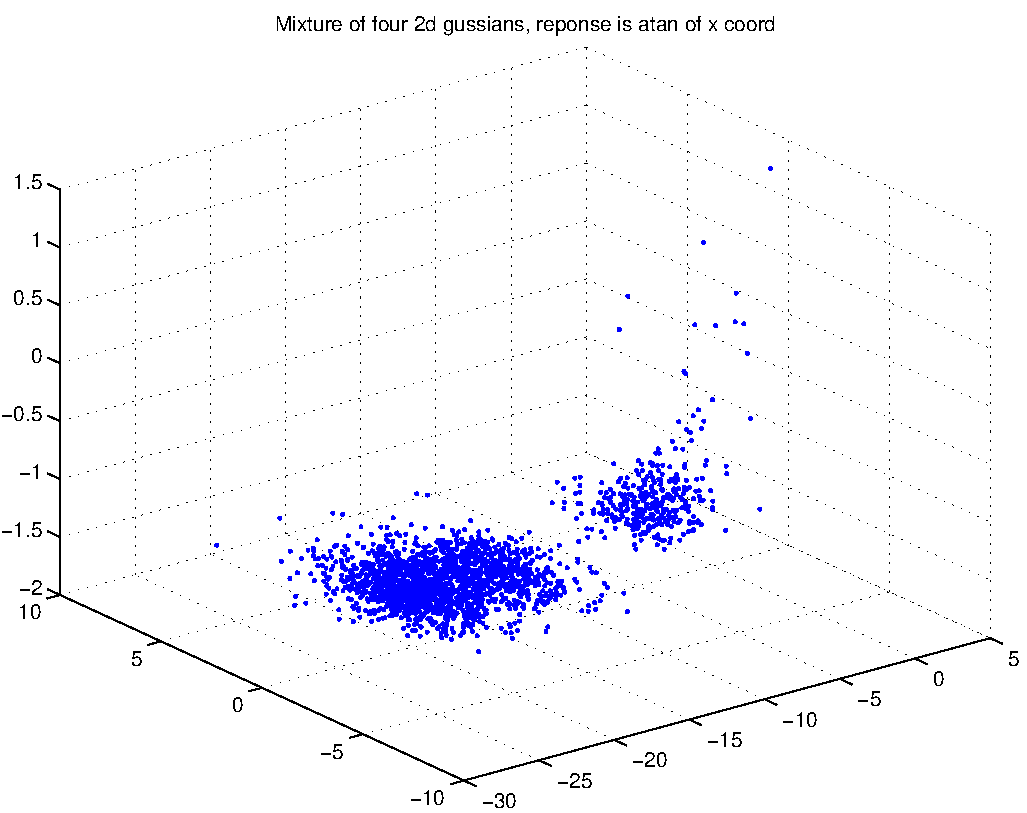
\includegraphics[width=10.0cm,height=10.0cm]{AtanDataSet.pdf}

\subsubsection{3 x 1 Linear Regression}
Sample size = 4000

Number of features = 3

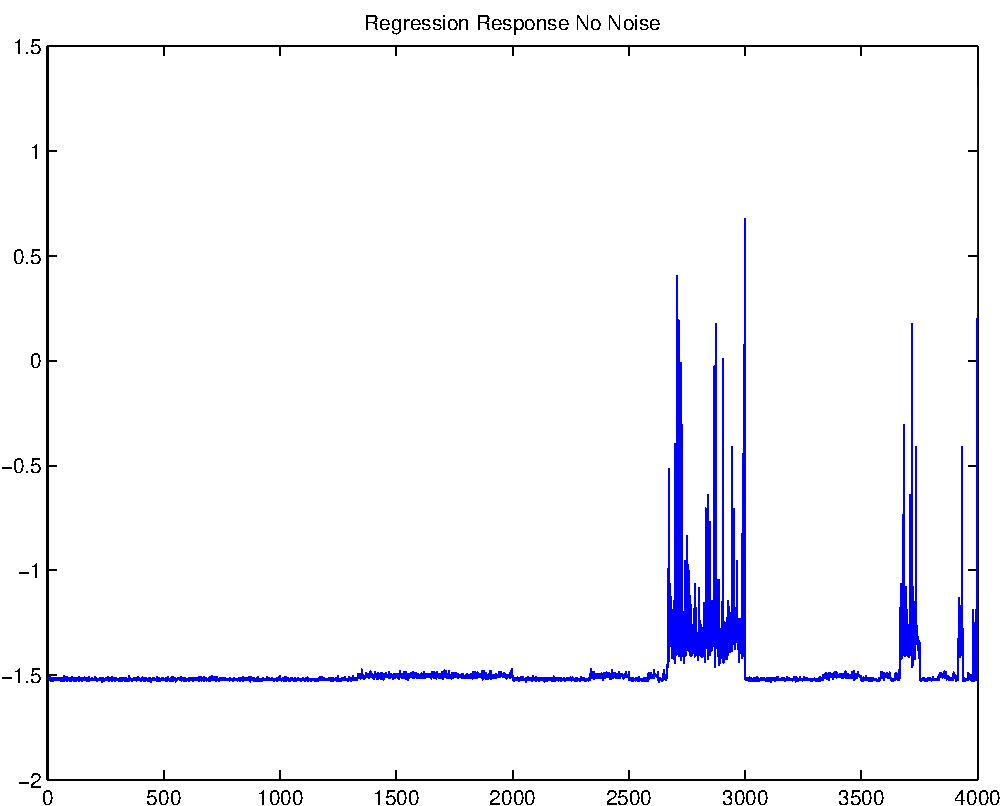
\includegraphics[width=10.0cm,height=10.0cm]{AtanDataSet_regression_response_no_noise.pdf}

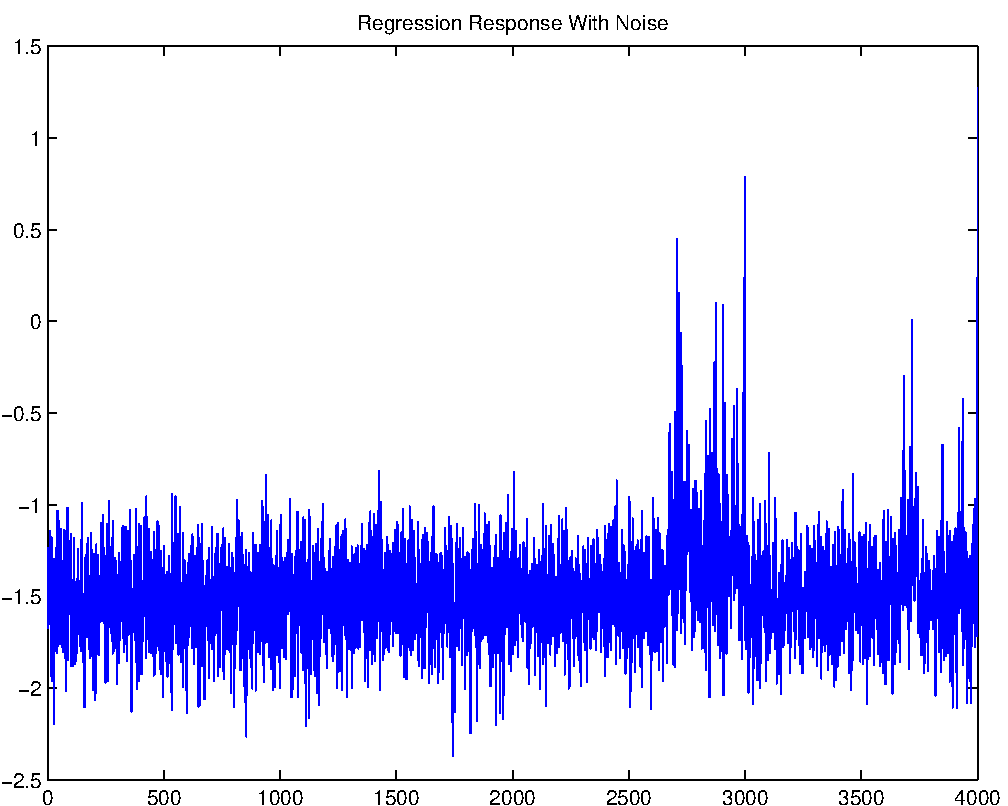
\includegraphics[width=10.0cm,height=10.0cm]{AtanDataSet_regression_response_with_noise.pdf}

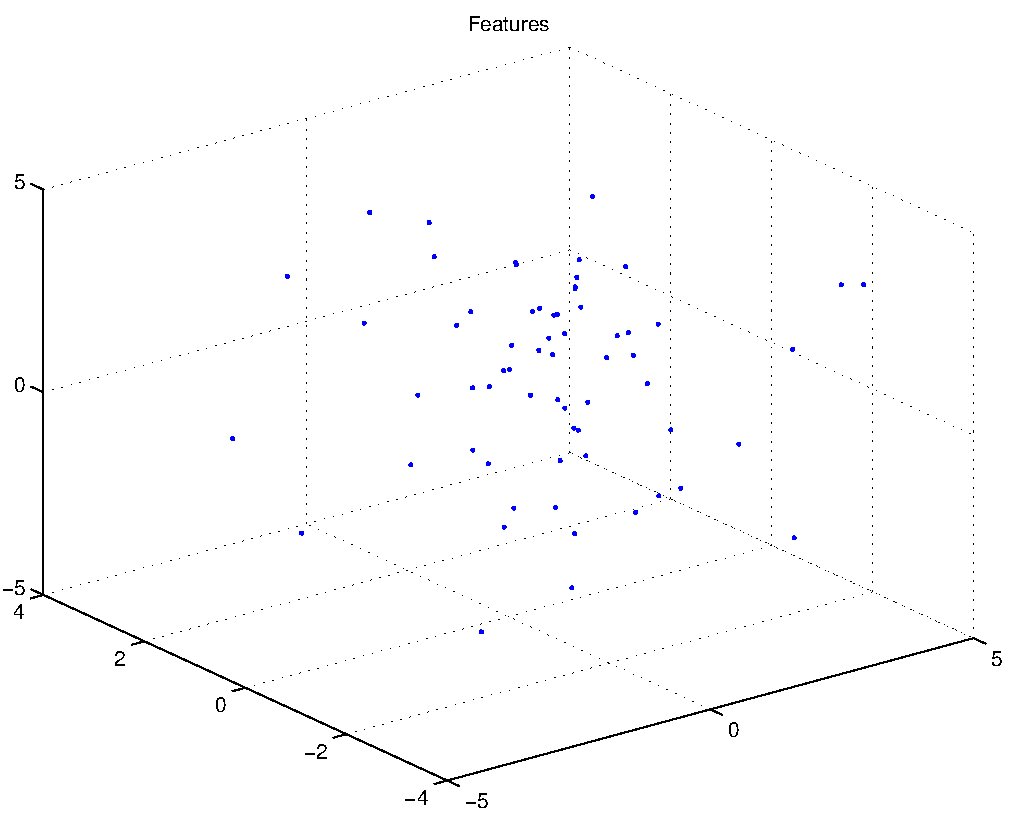
\includegraphics[width=10.0cm,height=10.0cm]{regression_features.pdf}

Response
-1.43849
-1.6586
-1.41849
1.57679
-1.3108
-1.32815
-1.14388
1.59878
-1.32434
-1.14571
-1.60205
0.411587
-1.7418
-1.48714
-1.20946
0.928197
-1.17449
-1.36349
-1.76913
1.23897
-1.42283
-1.51459
-0.986019
1.04558
-1.47216
-2.16325
-0.903734
1.52098
-1.45389
-1.74911
-1.26633
1.54642
-1.80702
-1.77582
-1.50188
1.59477
-1.26183
-1.48562
-1.13369
1.05421
-1.15027
-1.33376
1.29825
1.70808
-1.23341
-1.76475
-1.38489
1.07516
-1.52484
-1.06755
-1.23839
1.53843
-1.55082
-1.73154
-0.898088
1.25582
-1.45454
-1.11978
-1.45776
1.18233
-1.48728
-1.75151
-1.18003
1.26026
-1.81239
-1.28876
-1.37038
1.01491
-1.53552
-1.47869
-0.967694
1.72862
-1.74562
-1.22412
-1.54659
0.891589
-1.60517
-2.00655
-0.899375
1.28386
-1.43923
-1.51171
-1.44266
1.82672
-1.34522
-0.994919
-1.40822
1.37125
-1.85324
-1.5476
-1.35536
1.42705
-1.37846
-1.49913
-0.887049
1.33731
-1.37993
-1.21041
-0.892738
1.01293
-1.81016
-1.47911
0.802354
1.1338
-1.70302
-1.81992
-1.25342
1.30835
-1.61433
-1.61534
-1.70205
1.38072
-1.18334
-1.3688
-1.6548
1.02037
-1.81043
-1.3977
-1.59027
1.33969
-1.67091
-1.60702
-1.6241
1.13536
-1.79909
-1.5323
-1.32844
1.45324
-1.40553
-1.21344
-1.08189
1.31902
-1.69485
-1.63638
-1.06492
1.40279
-1.58531
-1.76747
-1.63371
0.938534
-1.66919
-1.4499
-1.12841
1.03516
-1.80172
-1.1764
-1.60295
1.75869
-1.62877
-1.75796
-1.63676
1.32797
-1.48859
-1.71922
-1.43269
1.12395
-1.67535
-1.46451
-1.80519
1.18712
-1.37745
-1.27148
-0.402464
1.51135
-1.68744
-1.58374
-1.19732
1.56075
-1.71605
-1.4832
-1.15668
1.3859
-1.37033
-1.16613
-0.915802
1.35508
-1.62513
-1.74984
-0.908471
1.5497
-1.49124
-1.57237
-1.60837
1.27154
-1.47902
-1.80067
-0.879096
1.66545
-1.55533
-1.43317
-1.53473
1.62499
-1.73449
-1.37251
-1.3134
1.39182
-2.01293
-1.39698
-1.3767
1.20139
-1.27148
-1.3487
-1.88999
1.07625
-1.35008
-1.39194
-1.8631
1.42137
-1.4611
-1.19916
-1.22213
1.623
-1.61435
-1.72254
-1.11006
1.41911
-1.51655
-1.80245
-1.61645
1.18401
-1.81822
-1.42273
-1.47187
1.2831
-1.44248
-1.36807
-1.33198
1.35631
-1.53401
-1.06982
-1.02422
1.53037
-1.39875
-1.16376
-1.50517
1.07385
-1.512
-1.41691
-1.0876
1.844
-1.48544
-1.52615
-1.54652
0.999097
-1.32383
-1.71733
-0.985561
1.44373
-1.96964
-1.50639
-1.33155
1.39964
-1.42637
-1.33354
-0.549639
1.3783
-1.33085
-1.55568
-1.08657
0.930513
-1.96422
-1.46593
-0.832915
1.46321
-1.66004
-1.17326
-1.15588
1.63293
-1.56709
-1.61716
-1.31271
1.5804
-1.62606
-1.42044
-1.4674
1.43063
-1.20227
-1.73696
-1.09101
0.594046
-1.35412
-1.45632
-1.00287
0.630135
-1.64254
-1.58483
-1.53171
1.26786
-1.51113
-1.34026
-1.06351
1.08785
-1.44258
-1.29647
-1.44249
1.22251
-1.42194
-1.47043
-1.74353
0.899861
-1.37852
-1.44106
-1.39969
1.29849
-1.67648
-1.59033
-0.989274
1.02396
-1.4545
-1.72633
-1.08511
1.432
-1.64223
-1.3171
-1.42154
1.11048
-1.57913
-1.48451
-0.95699
1.78979
-1.50084
-1.4941
-1.33673
1.50644
-1.12077
-1.57377
-1.39638
1.02917
-1.41537
-1.59016
-1.39083
1.4393
-1.41794
-1.54864
-0.959039
1.1584
-1.41027
-1.17454
-1.08836
1.65173
-1.42447
-1.1671
-1.71713
1.44638
-1.13546
-1.61015
-1.45699
1.13373
-1.41278
-1.424
-1.59693
1.3366
-1.45825
-1.22066
0.316617
1.86398
-1.60283
-1.46881
-1.31631
1.38045
-2.11857
-1.41737
-1.38785
1.40418
-1.45473
-1.66165
-1.24948
1.24719
-1.61952
-1.67984
-1.15909
1.223
-1.51529
-1.67645
-1.33075
1.41103
-1.58563
-1.71836
-1.6997
1.72652
-1.84959
-1.34186
-1.4002
1.13165
-1.59831
-1.61009
-1.08529
1.06528
-1.24675
-1.34876
-1.1969
0.863358
-1.774
-1.08855
-1.36541
1.61847
-1.61984
-1.86104
-1.44951
1.4208
-1.11166
-1.59882
-1.34926
0.944066
-1.674
-1.53356
-1.48301
1.29545
-1.59716
-1.47933
-1.63571
1.21902
-1.50416
-1.43743
-1.4655
1.47895
-1.07382
-1.31882
-1.13376
1.30646
-1.493
-1.79777
-0.318151
1.70654
-0.954162
-1.56706
-0.839242
1.14468
-1.2536
-1.40718
-0.777701
1.73896
-1.17442
-1.36165
-0.96555
1.25452
-1.80125
-1.67291
-1.27079
1.47073
-1.56835
-1.5862
-1.53166
1.4819
-1.24873
-1.38214
-1.62764
1.53587
-1.32676
-1.44973
-1.26594
1.41087
-1.84073
-1.64111
-1.43732
-0.0484158
-1.16031
-1.2299
-1.23926
0.977071
-1.89791
-1.53768
-1.71073
1.07441
-1.2515
-1.74233
-1.69772
1.08705
-1.53972
-1.1891
-1.28962
1.09168
-1.09256
-1.15524
-1.45071
1.09004
-1.39301
-1.1021
-1.35512
1.03483
-1.23175
-1.69758
-1.57791
1.56389
-1.72319
-1.50748
-1.24273
1.549
-1.93418
-1.45452
-1.52193
1.07524
-1.49764
-1.50907
-1.20603
1.36495
-2.04878
-1.31618
-1.41378
1.30898
-1.22833
-1.26995
-1.59264
1.26957
-1.77562
-1.55277
-0.85521
1.41171
-1.84989
-1.40137
-1.40535
1.27291
-1.82728
-1.6171
-1.2698
0.634785
-1.77225
-1.51113
-1.17924
1.42951
-1.27402
-1.78223
-1.23715
1.1186
-1.87191
-1.75877
-1.7554
1.08856
-1.39262
-1.49569
-1.30382
0.315259
-1.4054
-1.48083
-0.805587
1.17722
-2.10574
-1.30521
-0.812079
1.7102
-1.42816
-1.29224
-1.27392
1.15901
-1.49762
-1.44129
-1.44381
1.03117
-1.46312
-0.93254
-0.951491
1.18706
-1.75486
-1.53354
-1.54105
1.13299
-1.62691
-1.3847
-1.32016
1.20361
-1.45592
-1.14258
-1.59916
1.31967
-1.72407
-1.43036
-1.0554
1.30351
-1.01935
-1.55143
-1.55344
0.636993
-1.86801
-1.65109
-1.19773
1.03101
-1.55996
-1.55808
-1.57309
1.06906
-2.00663
-1.33575
-1.02976
1.01691
-1.51145
-1.53484
-1.56591
1.15147
-1.30923
-1.46343
-1.30182
0.920204
-1.48138
-1.56374
-0.935894
1.55155
-1.85577
-2.12653
-1.75165
1.24549
-1.7261
-1.51086
-1.21641
1.1082
-1.75589
-1.2852
-0.93997
1.30105
-1.72849
-1.2496
-1.52074
1.09757
-1.41084
-1.42078
-1.47613
1.53395
-1.23046
-1.4931
-1.35793
0.882171
-1.18295
-1.26457
-0.990789
1.63508
-1.53071
-1.34582
-1.28606
0.621141
-1.31422
-1.84151
-1.46907
1.2409
-1.28531
-1.6663
-1.06208
1.57119
-1.44822
-1.73469
0.25014
1.5999
-1.76857
-1.24594
-0.749146
1.61987
-1.52211
-1.74861
-1.60352
1.63077
-2.10553
-1.27129
-1.45078
0.554596
-1.19324
-2.08671
-1.09238
1.18928
-1.43353
-1.55695
-1.5587
1.16368
-1.43697
-1.68847
-1.15324
0.98323
-1.10906
-1.28217
-1.57567
1.49591
-1.32015
-1.62409
-1.59936
0.908661
-1.43338
-1.72036
-0.669961
1.37162
-1.82654
-1.83438
-1.67101
1.17474
-1.63046
-1.64533
-1.27715
1.54183
-1.46199
-1.40114
-1.08145
1.5834
-1.73601
-1.46373
-1.05486
1.58958
-1.94567
-1.23137
-1.38584
1.0429
-1.43904
-1.72739
-1.64874
0.84271
-1.40239
-1.54917
-1.545
1.2312
-1.42358
-1.39054
-1.33591
1.67608
-1.78832
-1.404
-1.52559
1.11638
-1.72077
-1.37467
-1.74235
1.03127
-1.40533
-1.65864
-1.07933
1.14452
-1.49188
-1.28788
-0.931742
1.41795
-1.51901
-1.4055
-1.47291
1.05908
-1.28927
-1.53758
-0.993863
0.884362
-1.53108
-1.41647
-1.17993
1.24461
-1.52362
-1.57232
-1.13825
1.04927
-1.32236
-1.72093
-1.08951
1.48072
-1.27778
-1.56855
-1.4041
1.37904
-1.45969
-1.39085
-1.06503
1.25826
-1.43206
-1.89316
-1.00744
1.76907
-1.52146
-1.81844
-0.972056
0.969334
-1.33184
-1.62577
-1.23954
1.036
-1.18025
-1.62805
-1.50511
1.4245
-1.54562
-1.65397
-1.22169
1.02341
-1.77807
-1.50168
-1.41564
1.19408
-1.74032
-1.41264
-1.53723
1.64203
-1.32591
-1.78067
-1.44365
1.43324
-1.80631
-1.48491
-1.24522
1.3613
-2.03103
-1.4717
-1.54497
0.873371
-1.64314
-1.68807
-0.975604
1.14502
-1.51539
-1.25997
-0.805709
1.09598
-1.40957
-1.77654
-1.61579
1.04947
-1.41721
-1.63751
-1.24709
0.861131
-1.1836
-1.18204
-1.12713
1.06772
-1.58531
-1.56462
-0.792004
1.33433
-1.33552
-1.37496
-1.30223
1.55088
-1.08691
-1.49961
-1.38663
1.37969
-1.47172
-1.30622
-1.54715
1.36741
-1.56174
-1.89137
-1.38288
1.31008
-1.16899
-1.43689
-0.887953
1.4393
-1.15488
-1.29973
-1.36516
0.90098
-1.44461
-1.26252
-1.40402
1.23952
-1.987
-1.30941
-1.3157
1.29468
-2.08474
-1.56606
-1.57946
1.62943
-1.62195
-1.57463
-2.0317
1.13361
-1.80058
-1.41369
-1.18909
1.15745
-1.53147
-1.73728
-1.53493
1.28254
-1.47912
-1.29085
-1.52416
1.54839
-1.65243
-1.80646
-1.2612
1.42801
-1.67108
-1.33579
-1.10996
1.03087
-1.692
-1.50191
-1.68029
1.18607
-2.00413
-1.12954
-1.30185
1.10244
-1.35114
-1.40549
-1.51016
1.03695
-1.65476
-1.31239
-1.4041
1.3691
-1.56409
-1.182
-1.60201
1.48952
-1.45455
-1.18893
-1.08767
1.64076
-1.80424
-1.61932
-1.09314
1.56612
-1.81552
-1.78302
-1.10663
1.17943
-1.60199
-1.36928
-1.61255
1.29231
-1.29886
-1.20753
-1.71083
1.144
-1.53597
-1.45839
-0.93944
1.22346
-1.3859
-0.945763
-1.07907
1.69147
-1.5782
-1.43471
-0.907748
0.976019
-1.87634
-1.6927
-1.70115
1.10144
-1.75397
-1.58685
-1.14326
1.34752
-1.09818
-1.39004
-1.2119
1.12866
-0.83567
-1.73408
-1.23951
1.35514
-1.54884
-1.51795
-0.197545
1.33941
-1.51992
-1.44988
-1.69739
1.26497
-1.39876
-1.21805
-1.11632
1.58237
-1.82695
-1.66258
-1.22384
1.32152
-1.89542
-1.06943
-1.38307
1.56364
-1.6777
-1.30996
-1.49919
1.56583
-1.69189
-1.39072
-1.91999
0.708087
-1.59415
-1.71307
-1.25112
0.869661
-1.55753
-1.63868
-1.04243
1.39614
-1.27975
-1.43671
-1.39994
1.29481
-1.13064
-1.23568
-1.1621
1.35104
-1.48356
-1.43076
-1.26259
1.27348
-1.34469
-1.37338
-1.56477
1.54111
-1.60103
-1.18573
-0.944597
1.24061
-2.00376
-1.66337
-0.953222
0.87649
-1.60857
-1.58573
-0.998821
1.4781
-1.77855
-1.32149
-1.38662
1.30632
-1.3583
-1.47165
-1.20935
1.38189
-1.82485
-1.44654
-1.36365
1.5246
-1.30036
-1.67864
-1.23975
1.21479
-1.5578
-1.54861
-1.72601
1.47209
-1.53352
-1.43051
-0.628097
1.47271
-1.39447
-1.57145
-0.790531
1.32158
-1.24511
-1.42932
-0.682926
1.64178
-1.52293
-1.47597
-1.49667
1.21803
-1.57949
-1.51905
-1.4834
1.35645
-2.0511
-1.57321
-1.48206
1.63676
-1.45263
-1.99836
-1.63328
0.85985
-1.73485
-1.42303
-1.47735
0.81863
-1.37846
-1.39475
-1.30497
1.2264
-1.93605
-1.31672
-1.08145
1.24012
-1.39222
-1.25088
-0.965262
1.71764
-1.70771
-1.38199
-0.936669
0.57546
-1.84081
-1.51395
-1.26604
1.2811
-1.49637
-1.64003
-1.05506
1.3623
-1.60241
-1.61341
-0.808478
1.57427
-1.37878
-1.42642
-0.432703
1.13582
-1.49442
-1.43083
-1.34805
1.53356
-1.29176
-1.35231
-1.67277
1.56901
-1.90011
-1.33248
-1.15034
1.02871
-1.08221
-1.7744
-1.21553
0.82104
-1.53209
-1.3053
-2.01344
1.09394
-1.54583
-1.49331
-1.64346
1.43976
-1.33044
-1.88284
-1.40995
0.966348
-1.54775
-1.28205
-1.47932
0.691158
-1.03039
-1.56639
-0.895712
1.29807
-1.79127
-1.57663
-1.6527
1.26517
-1.49527
-1.86712
-1.28464
1.21137
-1.41126
-1.54406
-1.3258
1.14635
-1.37503
-1.20966
-1.10229
1.37712
-1.65956
-1.24414
-1.32489
0.937973
-1.39511
-1.48078
-1.7502
1.31232
-1.35346
-1.79629
-1.02316
1.20529
-1.65467
-1.30035
-1.10321
0.743868
-1.77478
-1.12781
-1.65793
0.287225
-1.74376
-2.05765
-1.46221
1.59046
-1.58646
-1.52771
-0.685212
1.11329
-1.47317
-1.33973
-1.41339
1.4013
-1.17921
-1.5755
-0.944693
1.51272
-1.5891
-1.19176
-0.0353923
1.39366
-1.33351
-1.40462
-1.244
1.15489
-1.53892
-1.27662
-1.20749
1.34568
-1.63391
-1.59786
-1.44023
1.31648
-1.7345
-1.70609
-1.46345
0.990688
-1.36185
-1.45579
-1.29167
1.45306
-1.45269
-1.51116
-1.25841
1.31351
-1.51611
-1.46159
-1.45645
1.53641
-1.18676
-1.34299
-1.2508
1.32512
-1.61661
-1.3387
-1.37564
0.904774
-1.65436
-1.80857
-1.14377
1.31895
-1.77336
-1.70309
-1.11231
0.97948
-1.27495
-1.34931
-0.282997
1.44306
-1.44909
-1.42966
-1.21374
1.69484
-1.52182
-1.34177
-1.12158
1.08648
-1.17885
-1.2941
-1.00741
1.28301
-2.00335
-1.39105
-1.27085
1.77003
-1.54744
-1.46763
-1.64235
0.872187
-1.62489
-1.59458
-1.32456
1.55715
-1.2583
-1.6532
-1.07504
0.939131
-1.67323
-1.15814
-1.4792
0.950962
-2.014
-1.49775
-1.05993
1.45242
-1.46187
-1.44375
-0.972922
1.21235
-1.66138
-1.62964
-1.21471
1.20704
-1.5987
-1.64193
-1.36112
1.04291
-1.07847
-1.70909
-1.11997
1.76732
-1.32857
-1.69865
-1.48625
0.777463
-1.5002
-1.34884
-1.65333
1.25412
-1.39459
-1.541
-1.63106
1.19816
-1.55732
-1.68979
-1.02796
1.17768
-1.53673
-1.30276
-1.50527
1.23723
-1.61509
-1.62874
-1.62563
1.58797
-1.99505
-1.57798
-0.955707
1.52255
-1.51306
-1.26116
-1.35501
1.48001
-1.46094
-1.80245
-1.26659
1.03588
-1.72331
-1.27582
-1.05853
1.06915
-1.74798
-1.20272
-1.08659
1.21425
-1.66183
-1.64022
-0.0200754
1.49664
-1.7851
-1.23111
-1.63164
1.01086
-1.5689
-1.46674
-1.0247
1.52042
-1.66297
-1.52043
-1.11756
1.13262
-1.44333
-1.31454
-1.21938
1.24783
-1.27441
-1.23385
-1.33825
1.68988
-1.6562
-1.39203
-1.50147
1.39839
-1.39259
-1.29965
-1.18898
1.54012
-1.52836
-1.67189
-1.07347
1.02618
-1.96797
-1.23274
-1.37376
1.2274
-1.54183
-1.59861
-1.4584
1.44613
-1.53858
-1.20892
-0.786435
1.56245
-2.00376
-1.68606
-1.15813
1.35148
-1.65152
-1.10247
-1.33333
1.51478
-1.55547
-1.33568
-1.55298
1.81791
-1.19034
-1.18132
-1.49626
1.23665
-1.56959
-1.32718
-1.72442
1.46408
-1.35759
-1.63444
-1.08208
0.787814
-1.21599
-1.41402
-1.25938
1.29868
-1.0767
-1.81959
-1.80123
1.16181
-1.68962
-1.37437
-0.818026
1.39469
-1.38258
-1.12405
-1.47553
1.1404
-1.75508
-1.16178
-1.39292
1.24932
-1.38286
-1.46199
-1.19032
1.92907
-1.31717
-1.52917
0.0582118
1.41095
-1.73967
-1.2244
-1.82881
1.33289
-1.00693
-1.35833
-1.28086
1.3967
-1.7099
-1.53692
-1.05829
1.1919
-1.37967
-1.84448
-1.12169
1.5175
-1.46115
-1.48855
-1.6759
1.43558
-1.7753
-1.72731
-1.30689
1.02912
-1.28483
-1.58925
-1.10017
1.46223
-1.65074
-1.78629
-1.31715
1.64002
-1.71729
-1.50029
-0.675091
1.11423
-1.48543
-1.43904
-1.52146
0.997046
-1.34252
-1.30995
-1.47586
1.55323
-1.64464
-1.69353
-1.39464
1.54182
-1.45607
-1.63135
-0.831357
1.38605
-1.31072
-1.2788
-1.35881
1.39815
-1.7746
-1.42298
-1.19312
1.57335
-1.52231
-1.48005
-1.02739
1.31874
-1.16043
-1.34214
-1.40906
1.17921
-1.29226
-1.54074
-1.31259
1.17646
-1.42843
-1.09191
-1.3468
1.64008
-1.24559
-1.59649
-0.90582
1.31034
-1.70647
-1.27245
-1.26864
1.13555
-1.64215
-1.5348
-1.27229
1.21684
-1.55827
-1.82721
-1.37227
1.32596
-1.1589
-1.35731
-0.940199
1.20378
-1.65993
-1.58972
-1.19284
1.83805
-1.43673
-1.50214
-1.63616
1.33382
-1.96078
-1.33062
0.781581
1.10742
-1.57192
-1.18577
-1.50948
1.07803
-1.32844
-1.55332
-1.2916
0.808524
-1.3873
-1.61775
-1.39851
1.32026
-1.78578
-1.34554
-1.03018
1.16517
-1.20193
-1.4335
-1.11179
1.16006
-1.81827
-1.01265
-1.65729
1.19825
-1.59287
-1.58659
-1.58061
1.11558
-1.12038
-1.2842
-1.19498
1.67907
-1.4357
-1.4947
-1.74324
0.328692
-1.58835
-1.63821
-1.49328
1.60544
-1.34397
-1.29015
-1.30139
1.21744
-1.75717
-1.68553
-1.216
1.36456
-1.69457
-1.70078
-1.57613
0.977113
-1.44976
-1.48223
-1.46755
1.43413
-1.8573
-1.0819
-1.19063
1.03652
-1.63039
-1.25539
-1.78533
1.15333
-1.72999
-1.382
-1.46982
1.22526
-1.3336
-1.54524
-1.47975
1.26335
-1.27905
-1.92732
-0.932633
1.48431
-1.59779
-1.47064
-1.60696
0.985439
-1.17811
-1.46597
-1.16175
1.62625
-1.92441
-1.12842
-1.36296
1.00397
-1.63911
-1.45124
-1.44093
1.35122
-1.59481
-1.49793
-1.10434
0.770658
-1.52298
-1.21336
-1.5041
1.31847
-1.36909
-1.3452
-1.1568
1.29645
-1.99516
-1.75663
-1.46677
1.14837
-1.47174
-1.66362
-1.75841
0.59993
-1.5425
-1.59897
-1.25919
1.56426
-1.62843
-1.42847
-1.80219
1.22406
-1.80595
-1.6027
-1.59145
1.75184
-1.39751
-1.3914
-1.49339
1.46679
-1.69916
-1.8858
-1.23175
0.859563
-1.75038
-1.266
-1.49374
1.56965
-1.304
-1.61503
-1.34991
1.33152
-1.50278
-1.64218
-1.12884
0.921672
-1.64058
-1.31332
-1.23509
0.969524
-1.76041
-1.49526
-1.41388
1.4854
-1.61447
-1.35003
-1.19329
1.051
-1.7022
-1.26932
-1.15599
1.02826
-1.72316
-1.77096
-1.54337
0.838187
-1.46183
-1.53532
-1.49308
1.15114
-1.71636
-1.63106
-1.49406
1.24954
-1.13128
-1.36283
-1.24961
1.30442
-1.5044
-1.23768
-1.58822
1.30672
-1.60103
-1.25196
-1.63491
1.44073
-1.29517
-1.34628
-1.17029
1.52958
-1.69954
-1.16666
-0.872852
1.82754
-1.58058
-1.30609
-1.09666
0.904183
-1.70131
-1.66095
-0.823257
1.30448
-1.4602
-1.64047
-1.44597
1.49736
-1.96211
-2.36396
-0.707825
1.45847
-1.80122
-2.00573
-1.53062
1.2272
-1.56341
-1.73672
-1.47693
1.12225
-2.15362
-2.02316
-1.25766
0.793197
-1.56795
-1.49414
-1.25704
1.04383
-1.41202
-1.1107
-1.46242
1.39163
-1.72488
-1.74465
-1.41838
1.06794
-1.38114
-1.63307
-1.36608
1.48957
-1.18314
-1.17537
-0.836777
1.53982
-1.66195
-1.57282
-1.09221
1.41638
-1.87484
-1.61571
-1.74177
1.33422
-1.22541
-1.11829
-1.24491
1.3925
-1.54606
-1.45927
-1.53358
1.05447
-1.3882
-1.4535
-1.26277
1.45426
-2.00856
-1.31561
-1.55675
1.24097
-1.69093
-1.49434
-1.48386
1.0187
-1.83514
-1.24979
-1.34323
1.36179
-1.38986
-1.78835
-1.12214
1.28385
-1.45406
-1.64769
-1.59041
1.50173
-1.65853
-1.88327
-2.13822
1.25414
-1.57123
-1.34417
-0.934343
1.68251
-1.36128
-1.66889
-1.17854
1.47759
-1.66853
-1.17559
-0.914812
1.65619
-1.67455
-1.61538
-1.18823
1.33195
-1.72325
-0.997216
-1.46629
1.13983
-1.28327
-1.16103
-1.26596
1.07393
-1.69584
-1.71026
-1.36789
0.677522
-1.36079
-1.33191
-1.71436
1.03494
-1.50315
-1.41278
-1.43317
1.77455
-1.88066
-1.53165
-1.09168
1.3749
-1.90447
-1.73911
-1.17634
1.56258
-1.56356
-1.41119
-1.28552
1.18621
-1.2962
-1.43348
-1.59903
1.22552
-1.37227
-1.25092
-1.18776
1.44476
-1.52354
-1.46513
-1.1647
1.74368
-1.59754
-1.43504
-1.4094
1.67825
-1.53091
-1.34136
-0.886066
1.36762
-1.50321
-1.09658
-1.01442
1.23169
-1.47186
-1.73704
-1.17382
1.34137
-1.11642
-1.81246
-1.38076
1.54681
-1.24237
-1.73391
-1.64152
0.981079
-2.02611
-1.57082
-1.19379
1.47252
-1.63692
-1.33534
-1.17838
1.0134
-1.39016
-1.6435
-1.71497
1.40511
-1.63275
-1.65527
-1.26263
1.60443
-1.35164
-1.67346
-0.846107
1.69076
-1.39412
-1.69097
-1.50817
1.33821
-2.22809
-1.16719
-1.47876
1.27372
-1.72795
-1.38699
-1.28271
1.24557
-1.38562
-1.29529
-1.71971
1.11989
-1.70624
-1.62074
-1.47662
1.33627
-2.15851
-1.48013
-1.3079
0.203803
-1.33692
-1.26616
-1.10719
1.67915
-1.39365
-1.60678
-0.963987
1.47286
-2.18115
-1.82566
-1.43472
1.59239
-1.28199
-1.14735
-1.63448
1.2806
-1.24816
-1.70936
-1.39942
1.22734
-1.27319
-1.29218
-0.480408
1.52183
-1.52341
-1.31958
-1.23538
1.25874
-1.69375
-1.39779
-1.45369
1.17498
-0.962742
-1.60302
-1.17957
0.959203
-1.43083
-1.72203
-1.53978
1.13301
-1.50108
-1.3932
-0.924651
0.996826
-1.32244
-1.32415
-1.29615
1.66986
-1.47135
-1.44903
-1.03883
1.09844
-1.28521
-1.78907
-1.37421
1.34629
-0.822215
-1.50488
-0.806151
1.10317
-1.77117
-1.35978
-1.3353
1.17659
-1.14391
-1.31607
-1.10905
1.48487
-1.73992
-1.3245
-1.12589
1.13588
-1.66593
-1.82557
-1.27107
1.19244
-1.55261
-1.48401
-1.43706
1.17518
-1.27649
-1.54496
0.855414
1.74428
-1.57871
-1.4187
-1.08918
1.36045
-1.55174
-1.6282
-1.05558
1.49755
-1.45011
-1.69611
-1.23438
1.22142
-1.75793
-1.28462
-1.0788
1.22757
-1.42682
-1.42308
-0.885044
1.507
-1.30251
-1.57234
-0.912189
1.38069
-1.44665
-1.59217
-1.29807
1.65952
-1.7096
-1.07642
-1.32731
0.508309
-1.43053
-1.72954
-1.53956
1.03737
-1.50684
-1.36696
-1.41277
0.77247
-1.42555
-1.7563
-1.33809
1.55162
-1.54414
-1.35889
-1.64714
1.13252
-1.54555
-1.33338
-1.00731
1.33417
-1.51174
-1.55579
-1.46098
1.46703
-1.41152
-1.4308
-1.26195
1.57089
-1.30339
-1.25137
-1.16459
0.894323
-1.78096
-1.78836
-1.1658
1.36876
-1.37109
-1.59207
-1.19909
1.23627
-1.36852
-1.67928
-1.43348
1.19576
-1.50926
-1.82296
-1.7106
1.37835
-1.62473
-1.65294
-1.07047
1.11455
-1.99722
-1.28666
-1.41163
1.56028
-1.58477
-1.41298
-1.60151
1.27631
-1.28687
-1.64267
-1.21794
1.09814
-1.30314
-1.84601
-0.648688
1.42954
-1.32617
-1.45394
-1.19881
1.56664
-1.46864
-1.48454
-1.17216
1.02107
-1.64239
-1.50546
-0.679063
0.824136
-1.69404
-1.41806
-1.43241
1.00923
-1.67449
-1.39251
-1.36887
1.26973
-1.43987
-1.45008
-1.16535
1.32948
-1.40035
-1.476
-0.975157
1.38382
-1.53336
-1.80284
-1.23933
1.6862
-1.75946
-1.09831
-1.12407
1.08785
-1.66867
-1.34283
-0.892252
1.59248
-1.2095
-1.63044
-1.10529
1.65554
-1.51102
-1.4043
-1.24549
1.47138
-1.87502
-1.56727
-1.246
1.12517
-1.38958
-1.53126
-1.20264
1.1554
-1.46929
-1.47558
-1.37189
1.20576
-1.80533
-1.64114
-0.984377
1.35953
-1.18856
-1.76282
-1.10519
1.77404
-1.74778
-1.4371
-1.4707
1.45918
-1.42062
-1.38156
-1.24022
1.19547
-1.56178
-1.53254
-0.949645
1.33365
-1.22681
-1.06911
-1.58651
1.12377
-1.5005
-1.73426
-1.5171
1.2745
-1.36002
-1.66483
-0.833019
0.974739
-1.72183
-1.59507
-1.23121
1.40115
-1.41115
-0.979746
-0.706704
1.65058
-1.65245
-1.45316
-1.01542
0.942073
-1.67554
-1.77315
-1.1058
1.22245
-2.0083
-1.66055
-1.23074
1.44898
-1.33848
-1.9694
-1.19974
1.49905
-1.28881
-1.27762
-0.0281011
1.44346
-1.53369
-1.46257
-1.15625
1.22872
-1.62656
-1.33426
-0.99455
1.22524
-1.63339
-1.71661
-1.58693
0.753657
-1.4707
-1.72984
-1.48968
1.49096
-1.54177
-1.50657
-0.92671
1.36245
-1.64505
-1.69483
-1.29826
1.54572
-1.49031
-1.38011
-1.0819
1.75339
-1.72219
-1.74242
-1.55483
1.02557
-1.62842
-1.28773
-0.473646
1.34556
-1.90222
-1.35398
-1.39098
1.07946
-1.9928
-1.4087
-1.3451
1.30624
-1.54394
-1.48285
-1.383
1.33824
-1.44468
-1.51835
-1.15917
1.59277
-1.25165
-1.24833
-1.64187
1.44034
-1.47959
-1.36717
-1.44057
1.66173
-1.32953
-1.726
-0.889185
1.34694
-1.51667
-1.30241
-1.12807
1.43709
-1.48135
-1.94953
-1.00514
1.29074
-1.5179
-1.3644
-1.29389
1.37135
-1.43072
-1.43473
-1.38157
1.22789
-1.41045
-1.42093
-1.68058
0.954728
-1.50399
-1.26124
-1.32205
0.991116
-1.47922
-1.67876
-1.12829
1.47129
-1.60531
-1.71856
-1.41948
1.41818
-1.31588
-1.72193
-1.18783
1.52328
-1.69494
-1.54546
-1.32862
0.735513
-1.55464
-1.39385
-1.66855
1.10523
-1.69994
-1.15627
-1.26674
1.55772
-1.38884
-1.57889
-1.00983
1.54632
-1.53078
-1.28926
-1.46301
1.39797
-1.49445
-1.51907
-1.08321
1.2749
-1.43048
-1.3734
-1.6148
1.44275
-1.35077
-1.48054
-1.2899
1.4512
-1.37261
-1.48181
-1.03278
1.25866
-1.57008
-1.39579
-0.44571
1.38958
-1.7875
-1.51931
-1.36312
1.70693
-1.29562
-1.54097
-1.78475
1.1121
-1.42751
-1.54987
-1.34885
1.46674
-1.59634
-1.43402
-0.635759
1.07061
-1.31576
-1.66252
-1.75399
1.27648
-1.33742
-1.11324
-1.1397
1.59179
-1.34759
-1.73865
-1.21738
1.1312
-1.46046
-1.12541
-1.5396
0.705725
-1.48001
-1.4902
-1.04219
1.40547
-1.46348
-1.65514
-1.05582
1.2791
-1.48401
-1.08168
-1.3228
1.55439
-1.41619
-1.55945
-1.30824
0.764336
-1.49478
-1.63534
-0.876577
0.909633
-1.58285
-1.692
-1.24999
1.78645
-1.29253
-1.56995
-1.4338
1.49448
-1.71743
-1.60032
-1.60478
1.19688
-1.45465
-1.31959
-0.839187
1.52496
-1.5377
-1.83656
-1.48205
1.12267
-1.72003
-1.66949
-1.25863
1.0621
-1.28381
-1.61149
-0.850046
1.3957
-1.44247
-1.44558
-1.64635
1.18659
-1.57607
-1.22572
-1.39256
1.27523
-1.60408
-1.45614
-1.55097
1.07025
-1.26272
-1.92232
-1.27231
1.37251
-1.55454
-1.84318
-1.44895
1.16679
-1.67029
-1.40695
-1.38804
1.41656
-1.71901
-1.52257
-0.968334
1.24952
-0.971447
-1.68787
-1.5149
0.762634
-1.56003
-0.959288
-0.936261
1.49162
-1.71009
-1.67369
-1.72439
1.68657
-1.68829
-1.82446
-1.2354
1.31239
-1.08627
-1.25552
-1.00661
1.1335
-1.70592
-1.67539
0.790624
1.61089
-1.62608
-1.79514
-1.70482
1.15586
-1.47371
-1.46245
-1.12333
1.2162
-1.4423
-1.65161
-1.51037
1.62368
-1.29061
-1.17826
-1.37244
1.05843
-1.32097
-1.31045
-1.3147
1.40807
-1.54566
-1.65348
-1.11749
1.30766
-1.25144
-1.87049
-1.07047
1.47211
-1.54581
-1.43464
-1.24917
0.945329
-1.02323
-1.0618
-1.37714
1.4402
-1.61401
-1.55711
-1.213
1.07863
-1.26184
-1.30888
-1.1213
1.39929
-1.68121
-1.29775
-1.39266
1.34019
-1.30913
-1.27107
-1.55027
1.5806
-1.39217
-1.22561
-1.39145
1.28771
-1.46987
-1.42069
-1.53236
0.854881
-1.66729
-1.44946
-1.23957
1.67769
-1.49173
-1.43853
-1.56147
0.96764
-1.83031
-1.69425
-1.9553
1.38335
-1.65447
-1.84346
-1.19715
1.38074
-1.67183
-1.6374
-0.864911
1.45144
-0.987626
-1.80718
-1.72703
0.539401
-1.09512
-1.75969
-0.989009
1.56552
-1.82759
-1.47774
-1.24518
1.65106
-1.27794
-1.13477
-1.34868
1.43608
-1.81577
-1.65517
-1.09956
1.48475
-1.47205
-1.18813
-0.951698
1.46788
-1.88141
-1.44328
-0.943265
1.48008
-1.24603
-1.68106
-1.23267
1.75964
-1.49764
-1.37216
-1.62269
1.49981
-1.43313
-1.48571
-0.723178
1.19463
-1.25821
-1.95005
-1.31416
1.1781
-1.40072
-1.43321
-1.2662
1.27036
-1.57731
-1.67038
-1.15471
1.41107
-1.45098
-1.31202
-1.28999
1.30155
-1.39003
-1.45571
-1.29721
1.35265
-1.16939
-1.5117
-0.857253
1.67635
-1.80392
-1.56638
-0.580619
1.59144
-1.6126
-1.59974
-1.40469
1.77673
-1.20905
-1.57856
-1.228
1.71179
-1.16682
-1.67478
-0.987166
1.99096
-1.5762
-1.70251
-1.20011
1.36724
-1.66935
-1.75872
-1.2102
0.953567
-1.4406
-1.96754
-1.27793
0.220141
-1.63346
-1.60049
-1.7431
1.42111
-1.72141
-1.73343
-0.95805
1.79518
-1.60264
-1.82008
-1.26742
1.23079
-1.41065
-1.38974
-1.3632
0.938968
-1.64587
-1.66199
-1.20841
1.73513
-1.15091
-1.07516
-1.46544
1.20607
-1.51493
-1.20671
-1.26236
0.959777
-1.41137
-1.56228
-1.20147
1.32352
-1.53948
-1.58369
-1.78898
1.48389
-1.74483
-1.17993
-1.40938
0.953757
-1.51875
-1.3609
-1.19799
1.20847
-1.4399
-1.35113
-1.71421
1.28028
-1.55821
-1.76905
-1.22936
1.46687
-1.35906
-1.19694
-1.04572
1.86888
-1.46017
-1.61434
-0.931752
1.76036
-0.989239
-1.37203
-1.158
1.41251
-1.56922
-1.52546
-1.17051
1.22089
-1.55042
-1.36061
-1.27702
1.28427
-1.41422
-1.9067
-1.89076
1.12253
-1.62717
-1.36058
-0.896908
1.2592
-1.60174
-1.28082
-1.75972
1.03673
-1.68357
-1.76852
-1.40804
1.40765
-1.36331
-1.27127
-0.848296
1.59081
-1.70008
-1.45405
-1.39722
1.13989
-1.69933
-1.10646
-1.3315
1.47439
-1.71992
-1.44801
-1.3153
1.54448
-1.46529
-1.71898
-1.12641
1.07161
-1.80852
-1.54166
-1.52117
1.26845
-1.11433
-1.51672
-1.47893
1.17553
-2.00493
-1.33066
-1.04269
1.32493
-1.7759
-1.94967
-1.36395
1.26881
-1.47338
-1.33087
-1.57298
1.07869
-1.73011
-0.915921
-0.946749
0.953662
-1.47279
-1.40691
-0.995337
0.783406
-1.84242
-1.54888
-1.66163
0.970063
-1.55526
-1.35058
-1.01413
1.2877
-1.27822
-1.63961
-1.39806
1.46163
-1.84984
-1.21841
-1.94685
1.56024
-1.23968
-1.75642
-1.68096
0.7197
-1.68274
-1.42285
-0.339511
1.25233
-1.59822
-1.06126
-0.880514
1.6213
-1.58212
-1.20707
-0.364503
1.07217
-1.30511
-1.22158
-1.52419
1.15657
-1.73323
-1.59487
-1.66548
1.21495
-1.66578
-1.29234
-1.32054
1.24912
-1.79879
-1.13138
-1.22088
1.13491
-1.08874
-1.63213
-1.76129
1.80208
-1.35102
-1.2951
-1.34199
1.57352
-1.36477
-1.83951
-1.69784
0.709459
-1.20296
-1.47261
-1.49182
1.59438
-1.57843
-1.44552
-1.66288
0.951518
-2.00429
-1.32964
-0.988939
1.34599
-1.42924
-1.6392
-0.890144
1.02352
-2.04398
-1.43028
-1.22559
2.14899
-1.61262
-1.1659
-1.3755
1.431
-1.54397
-1.6269
-0.912264
0.942852
-1.74119
-1.67814
-1.06123
0.477477
-1.19957
-1.55501
-1.59876
1.33426
-1.65806
-1.35452
-1.16537
1.34138
-1.62898
-1.34214
-1.30162
1.32058
-1.49168
-1.66526
-1.12721
0.961578
-1.28383
-1.49421
-1.20132
1.15009
-1.28521
-1.57193
-1.21475
0.912439
-1.09371
-1.34732
-1.05311
1.37195
-1.71546
-1.48025
-1.36716
1.33955
-1.50133
-1.76284
-1.10597
1.56891
-1.43431
-1.25672
-1.38231
1.37915
-0.924183
-1.54956
-0.697253
1.50013
-1.47536
-1.1461
-0.803899
1.57053
-1.65261
-1.81026
-1.59855
1.45775
-1.98152
-1.68735
-1.42431
1.47928
-1.62986
-1.64078
-1.34142
1.25785
-1.73899
-1.75551
-0.579248
0.994377
-1.85817
-1.07706
-1.43932
1.38899
-1.61953
-1.35576
-1.77147
0.805655
-1.23157
-1.39839
-1.37588
1.34966
-1.45674
-1.71919
-1.36047
1.54916
-1.79409
-1.28656
-1.05474
1.31708
-1.65526
-1.56429
-1.05759
1.53683
-1.40978
-1.74587
-1.91879
1.0428
-1.61721
-1.20545
-1.39723
1.2942
-1.49881
-1.8001
-1.20337
1.49576
-1.59875
-1.69561
-1.15102
1.4485
-1.47337
-1.27276
-1.37428
1.50113
-1.93948
-1.6365
-0.845884
0.598425
-1.56797
-1.54575
-0.886497
0.968162
-1.61346
-1.75617
-1.13392
1.57664
-1.57295
-1.55008
0.0596517
1.17282
-1.51496
-1.74845
-1.0486
0.935575
-1.55218
-1.55208
-0.648906
1.02163
-1.96241
-1.79585
-1.5662
1.38545
-1.80595
-1.53798
-0.958248
1.88267
-2.00072
-1.39938
-1.66902
1.54708
-1.50676
-1.52723
-1.06049
1.25465
-1.59175
-1.3518
-1.15633
1.63031
-1.27468
-1.53782
-1.00225
1.55038
-1.35883
-1.47717
-1.47479
1.21116
-1.64686
-0.945329
-0.364652
1.28006
-1.9589
-1.1835
-0.818437
1.36842
-1.57846
-1.2614
-1.31041
1.11419
-1.5003
-1.32365
-0.852379
1.06412
-1.79477
-1.50932
-0.550514
1.17074
-1.78664
-1.40647
-1.33251
1.59222
-1.81798
-1.58327
-1.3678
1.1305
-1.51916
-1.524
-1.17866
1.43822
-1.64969
-1.68625
-1.44652
1.18354
-1.21198
-1.39657
-1.4595
1.38113
-1.57707
-1.36543
-1.6677
1.17215
-1.38374
-0.923119
-0.183476
1.50112
-1.23553
-1.05018
-0.991197
0.959639
-1.51768
-1.5082
-1.38828
1.16696
-1.73752
-1.7086
-1.33878
1.05094
-1.44948
-1.39755
-1.19235
0.908932
-1.53609
-1.55152
-1.51551
1.24364
-1.51634
-2.00772
-0.941571
1.31592
-1.6413
-1.62919
-1.3804
1.37811
-1.19728
-1.39942
-1.51844
1.36133
-1.58434
-1.75646
-1.62013
1.07976
-1.58206
-1.53519
-1.06539
1.36363
-1.6833
-1.42668
-1.28025
1.28229
-1.53234
-1.52653
-1.4789
1.38338
-1.39906
-1.18685
-1.32887
1.10533
-1.24101
-1.70646
-1.09046
1.21516
-1.58795
-1.22962
-0.392331
1.53473
-1.91213
-1.87233
-1.46683
1.44696
-1.76696
-1.73908
-1.14548
1.67987
-1.25115
-1.37997
-1.04083
1.32223
-1.32552
-1.41368
-1.07098
1.32004
-1.49806
-1.59588
-1.18353
1.19517
-1.64201
-1.58299
-1.69557
0.946726
-1.057
-1.44499
-1.49798
1.07979
-1.24583
-1.32755
-1.14789
1.40825
-1.23616
-1.34322
-1.24481
1.27728
-1.42095
-1.23955
-1.66721
1.28623
-1.56141
-1.44613
-1.13239
1.52887
-1.8778
-1.65402
-1.07349
0.649375
-1.64682
-1.74239
-1.39066
1.38293
-1.79563
-1.51073
-1.72454
1.29843
-1.57028
-1.67768
-1.22014
1.2895
-1.71638
-1.59519
-1.33249
1.08193
-1.66605
-1.35069
-1.25611
1.24639
-1.50164
-1.49662
-1.08728
1.49088
-1.57816
-1.11046
-1.44007
1.38729
-1.47835
-1.11432
-1.39934
1.0535
-1.41538
-1.49545
-1.56444
0.575698
-1.39593
-1.60269
-0.488062
1.31485
-1.78913
-1.73081
-1.56865
1.26738
-1.77423
-1.26909
-1.49665
1.31562
-1.22596
-1.45115
0.365669
1.37994
-1.8237
-1.34021
-1.1424
1.77831
-1.78758
-1.23253
-0.798745
1.37353
-1.33636
-1.40481
-1.28125
1.28007
-1.43334
-1.28958
-1.36525
1.54164
-1.50638
-1.85746
-1.14336
1.45343
-1.10904
-1.6722
-1.38963
1.66396
-1.03805
-1.14775
-1.46316
1.11454
-1.62518
-1.35951
-1.36225
1.39411
-1.1601
-1.38416
-0.804186
0.993494
-1.78503
-1.51159
-1.1642
1.27685
-1.52188
-1.65169
-1.08437
1.6278
-1.25854
-1.70928
-1.42433
1.26431
-1.53495
-1.74838
-1.15254
1.21393
-1.82009
-1.57544
-0.929699
1.09291
-1.47622
-1.59739
-0.912697
1.18393
-1.70626
-1.51425
-1.5429
1.20209
-1.90458
-1.59314
-1.26683
1.03247
-1.60137
-1.13465
-1.28535
1.26946
-1.48525
-1.33871
-1.52621
1.52569
-1.43549
-1.72556
-1.49039
1.31722
-1.50684
-1.33785
-1.03223
1.04247
-1.53295
-1.76334
-0.020018
1.29684
-1.65264
-1.74509
-1.16248
0.734139
-1.1815
-1.20805
-1.25159
1.31104
-1.71151
-1.78452
-1.44886
1.26192
-1.99701
-1.34992
-1.65055
0.711744
-1.68144
-1.12903
-1.69782
1.01298
-1.90455
-1.15055
-1.31159
0.856426
-1.64623
-1.35796
-1.35209
1.35513
-1.84294
-1.46147
-1.52586
1.51748
-1.57052
-1.4803
-1.38966
1.1945
-1.3073
-1.73132
-0.518375
1.98849
-1.05639
-1.51849
-1.07556
0.945318
-1.8197
-1.14089
-0.609443
1.5551
-1.31809
-1.13213
-1.0609
1.44576
-1.69853
-1.5148
-1.16516
1.52956
-1.63131
-1.44278
-1.39364
1.12609
-1.43691
-1.2633
-1.36363
1.47853
-1.26177
-1.91707
-0.924787
1.36935
-1.27513
-1.61659
-1.12256
1.57127
-1.53535
-1.30726
-1.256
0.733611
-1.36075
-1.31722
-1.42647
0.930053
-1.58493
-1.8483
-1.21204
1.8746
-1.54552
-1.45587
-1.13919
1.37646
-1.31817
-1.24178
-1.54121
0.287285
-1.42803
-1.44422
-1.43564
1.15168
-1.69578
-1.3549
-1.24931
1.17402
-1.6599
-1.58254
-1.39057
1.12836
-1.71679
-1.55278
-1.33518
1.2143
-1.60741
-1.49936
-0.941106
1.76044
-1.3184
-1.81416
-1.18619
0.810911
-1.38105
-1.41847
-1.16624
1.21774
-1.31309
-1.59753
-1.18911
1.54187
-1.17779
-1.65144
-1.09403
1.25646
-1.86292
-1.3108
-1.04304
1.74614
-1.67798
-1.66335
-1.61904
0.961228
-1.45473
-1.3649
-1.33398
1.29703
-1.10188
-1.56529
-1.25253
1.49722
-1.34027
-2.05796
-1.09919
1.23514
-1.44748
-1.48885
-1.40311
1.22154
-1.63863
-1.18973
-1.38183
1.6262
-1.83305
-1.3009
-1.28661
1.33307
-1.31909
-1.64606
-1.19811
1.41212
-1.37713
-1.21962
-1.3128
0.964855
-1.72632
-1.55633
-1.51568
1.01302
-1.4331
-1.85535
-0.945086
1.19043
-1.49395
-1.24005
-1.29647
1.22715
-1.15728
-1.4419
-0.332655
1.77788
-1.43439
-1.66683
-1.35807
1.15627
-1.46737
-1.4062
-1.58865
1.49932
-1.65533
-1.3424
-1.57523
1.15331
-1.62523
-1.56462
-1.69839
1.39477
-1.31436
-1.83388
-1.30676
1.42727
-1.61998
-1.65461
-1.71867
1.33738
-1.86752
-1.43082
-1.41938
1.67089
-1.77314
-1.5854
-1.65142
1.25466
-1.28808
-1.05168
-1.55954
1.24779
-1.59648
-1.27055
-1.18634
0.826517
-1.80331
-1.22009
-1.43121
1.41695
-1.3963
-1.63429
-1.50325
1.31
-1.66028
-1.0482
-0.769092
1.22928
-1.85511
-1.28775
-0.91806
1.37082
-1.4543
-1.5505
-1.31802
1.24857
-1.42314
-1.16081
-1.07564
1.34552
-1.0767
-1.35276
-1.39144
1.3502
-1.63924
-2.01086
-0.960348
1.53762
-1.67642
-1.79825
-1.28487
1.16895
-1.64421
-1.60048
-1.70487
1.60936
-1.86393
-1.54719
-1.64589
1.57769
-1.34439
-1.58903
-0.456405
1.37874
-1.7626
-1.7014
-1.294
1.02122
-1.72207
-1.66326
-0.965959
1.54697
-1.13567
-1.76901
-1.64969
1.01996
-1.30713
-1.41286
-1.02702
1.21083
-1.41176
-1.43881
-1.33309
1.44415
-1.62103
-1.78439
-1.21308
1.19254
-1.68427
-1.67094
-1.63025
0.717031
-1.46412
-1.49908
-1.33516
1.79751
-0.962857
-1.60977
-1.30411
1.46408
-1.24989
-1.97505
-1.09905
1.40409
-1.53658
-1.28519
-0.074123
1.49159
-1.56688
-1.68658
-1.2487
1.13206
-1.6442
-1.7739
-1.02311
1.51409
-2.04035
-1.38655
-1.10963
1.60259
-1.19071
-1.54014
-0.943893
1.14631
-1.18208
-1.12394
-1.45075
1.43933
-1.57055
-1.43919
-1.31553
1.46948
-1.45103
-1.29446
-1.48126
0.369691
-1.38545
-1.423
-1.02136
1.012
-1.61684
-1.47763
-0.839408
1.24875
-1.51299
-1.23314
-1.29203
0.944802
-1.6363
-1.35004
-1.37929
1.29557
-1.58338
-1.28628
-1.19859
1.12804
-1.63951
-1.86795
-1.46224
1.05595
-1.8367
-1.79295
-1.40544
1.44903
-1.43655
-1.5652
-1.49504
1.41829
-1.37276
-1.60769
-1.13336
1.47161
-1.43085
-1.71837
-1.15796
1.24754
-1.81833
-1.05843
-1.06618
1.45477
-1.67132
-1.89731
-1.49718
1.46497
-1.85782
-1.73783
-1.15405
1.20482
-1.41068
-1.21697
-1.57709
1.35881
-1.26443
-1.5245
-1.19817
1.12927
-1.50891
-1.7033
-1.16563
0.97214
-1.42669
-1.28827
-0.957364
1.311
-1.67372
-1.33266
-1.21786
1.34745
-1.44517
-1.61352
-1.34689
1.18802
-1.58257
-1.44758
-1.32586
1.32565
-1.58784
-1.45304
-1.4642
1.46186
-1.68785
-1.5709
-1.21775
1.59659
-1.62974
-1.53335
-1.02756
1.56789
-1.64823
-1.53209
-1.7979
1.41874
-1.80263
-1.63576
-1.46865
1.61396
-1.41159
-1.50618
-0.857817
1.45187
-1.61164
-1.52064
-1.1276
1.58599
-1.18104
-1.70881
-1.68081
0.983905
-1.57944
-1.64174
-1.41075
1.0123
-1.11434
-1.75707
-1.15039
0.946227
-1.79479
-1.38295
-1.45264
1.17593
-0.692313
-1.41044
-1.45556
1.34484
-1.47731
-1.46129
-1.18072
0.660405
-1.40442
-1.39467
-1.3045
1.1858
-1.57164
-1.81833
-1.51116
1.26593
-1.72537
-1.71737
-1.3757
0.986358
-1.11764
-1.21565
-1.11507
0.580031
-1.44051
-1.80417
-1.31884
1.48688
-1.32618
-1.51244
-1.1711
0.85827
-1.14111
-1.53441
-1.52816
1.51164
-1.38057
-1.3536
-1.20828
1.65611
-1.98359
-1.48244
-1.39305
1.68702
-2.10057
-1.40843
-1.5217
1.20268
-1.37051
-1.66378
-1.24378
1.18686
-1.1872
-1.3029
-1.05448
1.37842
-1.14892
-1.4232
-1.82798
0.876359
-1.38471
-1.5038
-1.18778
0.793434
-1.65749
-1.4608
-1.03317
1.3601
-1.32236
-1.1842
-1.29985
1.99348
-1.78979
-1.65608
-0.70038
1.23173
-1.59314
-1.38651
-1.58264
1.15882
-1.57187
-1.48268
-1.14747
1.46857
-1.79531
-1.73377
-0.666195
1.32698
-0.588741
-1.66777
-1.72488
1.21849
-1.64791
-1.11851
-1.60796
1.17822
-1.30111
-1.50245
-0.833956
1.7792
-1.54145
-1.20121
-1.47114
1.15559
-1.78417
-2.06167
-1.23816
1.53019
-1.35863
-1.81133
-1.75824
1.3132
-1.94438
-1.54581
-0.992061
1.42608
-1.31873
-1.87457
-1.02108
0.907228
-1.64068
-1.8043
-1.98109
1.20451
-1.52048
-1.55865
-1.52172
1.33529
-1.70932
-1.20067
-1.33945
1.40355
-1.72389
-1.36098
-1.36442
1.34483
-1.59554
-1.62825
-0.90741
1.7455
-1.66458
-1.79646
-1.346
1.50286
-1.43364
-1.57016
-1.56599
0.133344
-1.07011
-1.37321
-0.632145
1.38822
Estimate for Beta
0.000158447
-0.00148263
0.99765
QueryPerformanceCounter  =  5.75189
\subsubsection{Linear Regression 3x1}
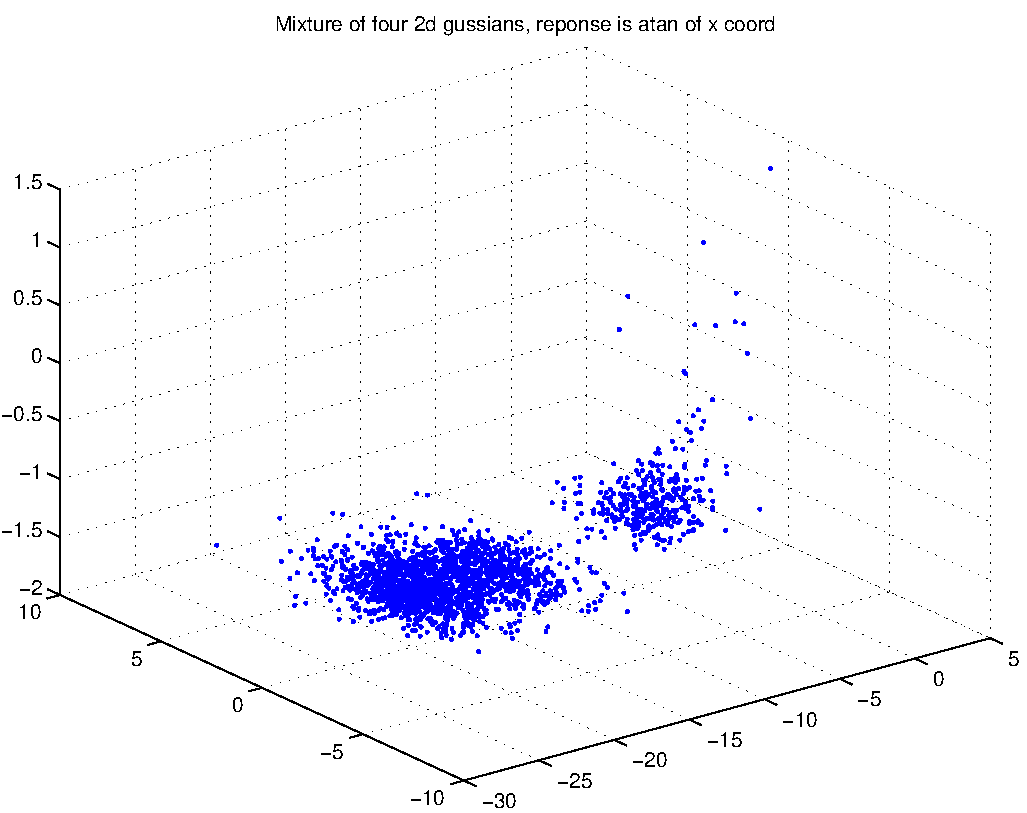
\includegraphics[width=10.0cm,height=10.0cm]{AtanDataSet.pdf}

\subsubsection{3 x 1 Linear Regression}
Sample size = 64

Number of features = 3

$\sigma = \left(
\begin{array}{
ccc}
+3.952 & -0.499 & -0.010 \\
-0.499 & +1.895 & +0.465 \\
-0.010 & +0.465 & +4.477 \\
\end{array}
\right)$ \newline 

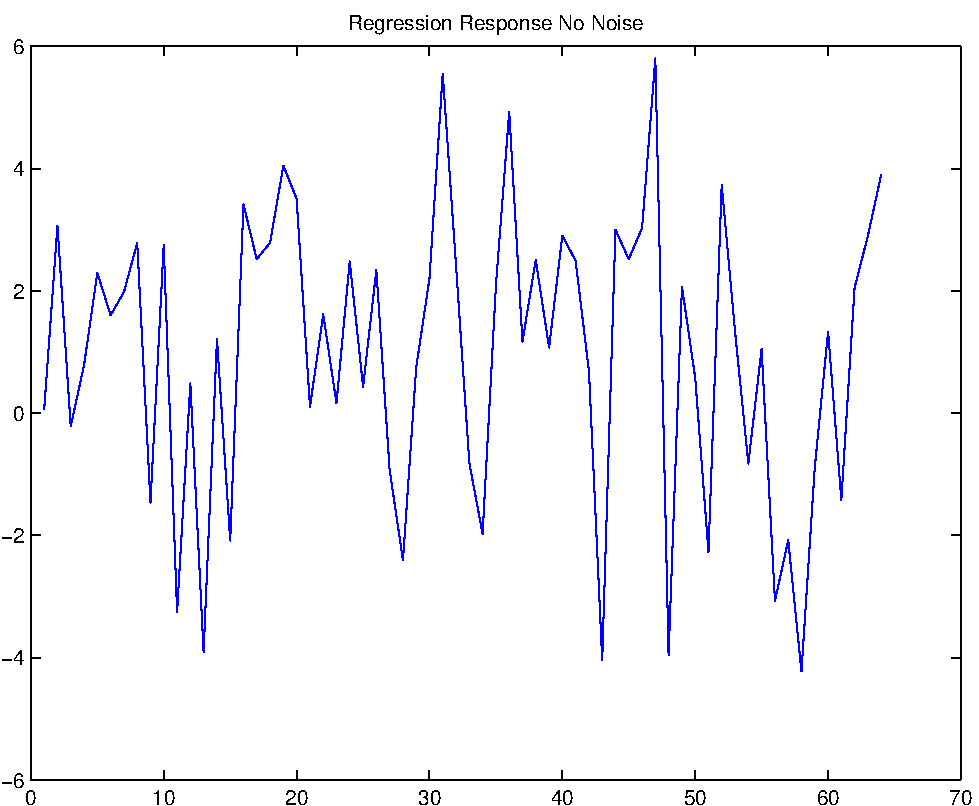
\includegraphics[width=10.0cm,height=10.0cm]{regression_response_no_noise.pdf}

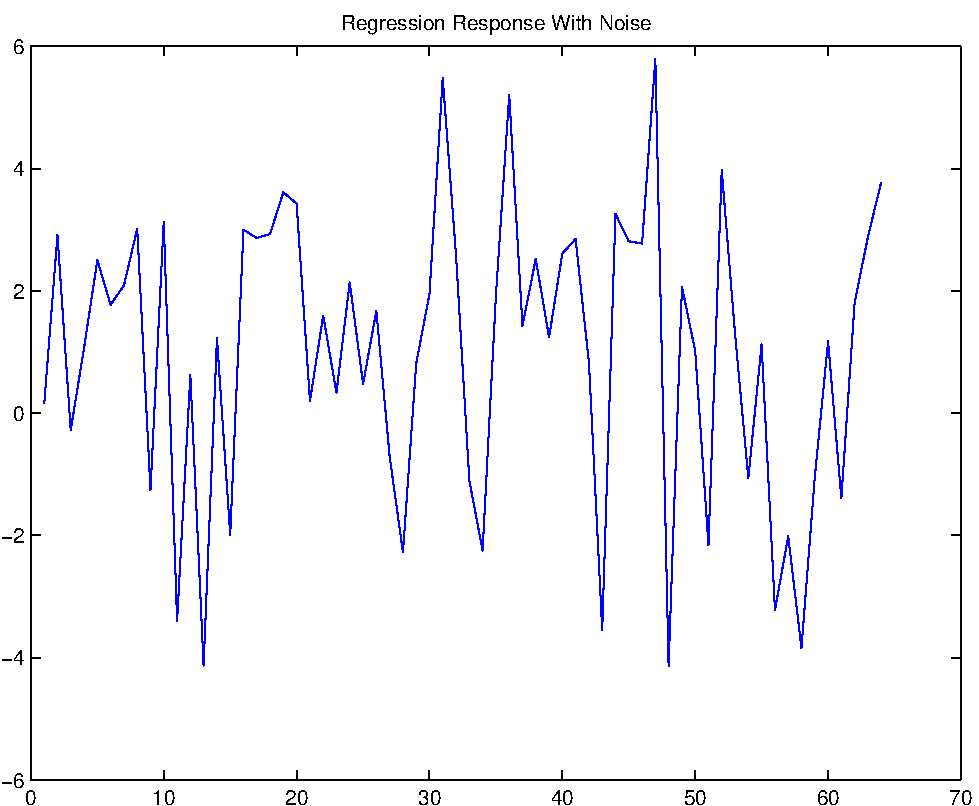
\includegraphics[width=10.0cm,height=10.0cm]{regression_response_with_noise.pdf}

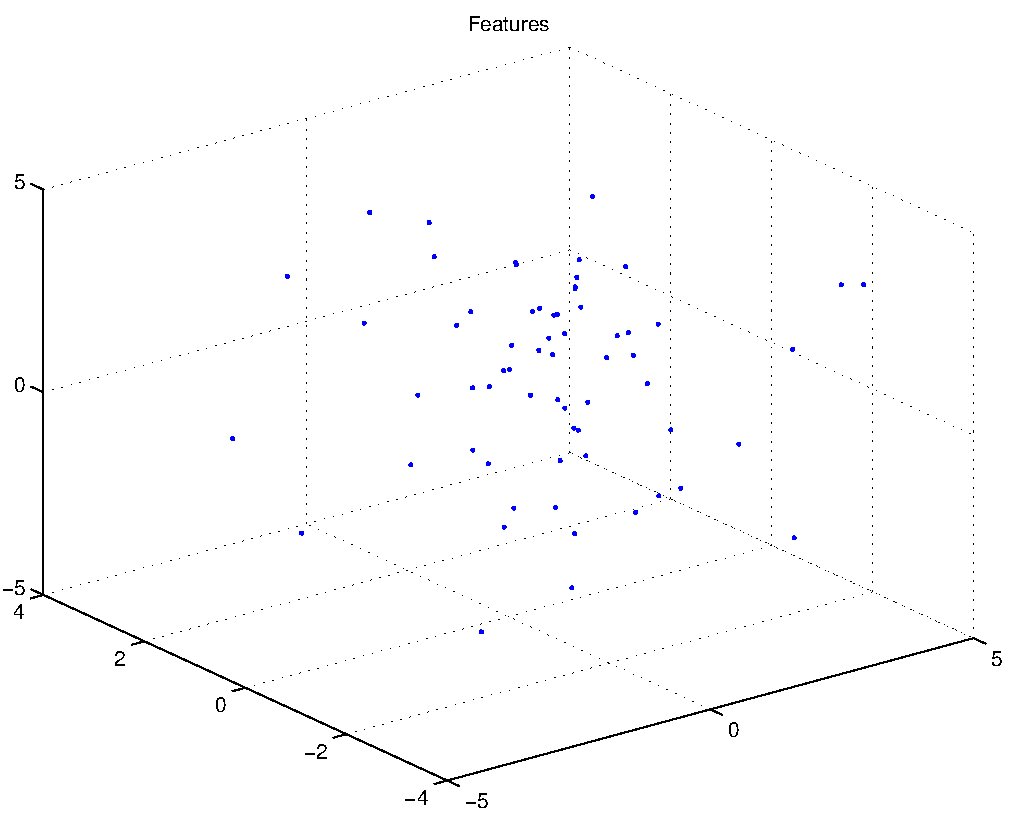
\includegraphics[width=10.0cm,height=10.0cm]{regression_features.pdf}

Beta
+0.817, +0.999, +0.510

Response
+0.373
+2.522
-0.790
+1.057
+0.707
+2.230
-1.023
+2.391
+1.803
+2.638
+1.978
+1.768
-0.992
+2.780
+0.071
+1.326
+1.069
+3.171
-0.464
+4.546
+3.854
+3.574
-0.481
+4.235
+1.998
+3.044
+0.268
+0.475
-0.333
+3.065
+2.497
+4.889
+2.108
-4.009
+0.741
+2.018
-0.341
+5.258
-6.550
-2.021
-1.858
+2.228
-2.827
+0.793
-1.754
-2.249
-2.680
+1.187
-1.962
+2.565
-4.014
+1.552
+0.936
-2.929
+0.117
-1.287
-2.091
+1.501
+0.592
+1.137
+1.371
+0.661
-0.223
+4.372
Estimate for Beta
+0.823
+0.996
+0.484
Error:
+0.006, -0.003, -0.027


QueryPerformanceCounter  =  +4.845
\subsubsection{Fast Gauss Transform}
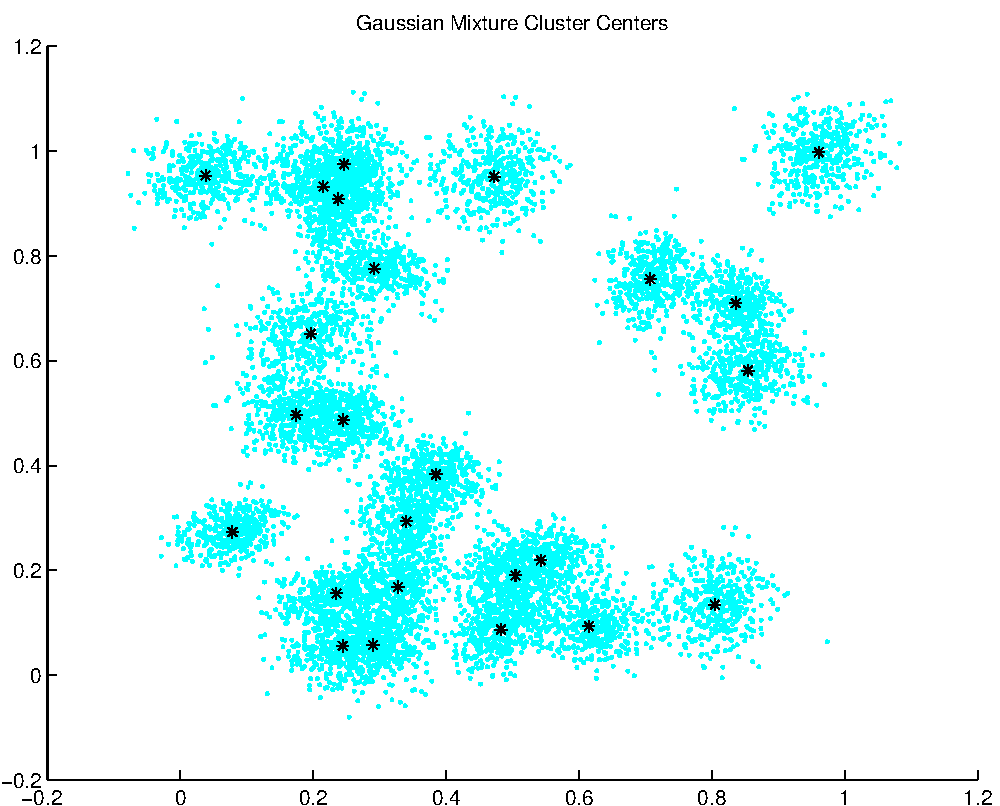
\includegraphics[width=10.0cm,height=10.0cm]{GaussianMixture_ClusterCenters25_Centers.pdf}

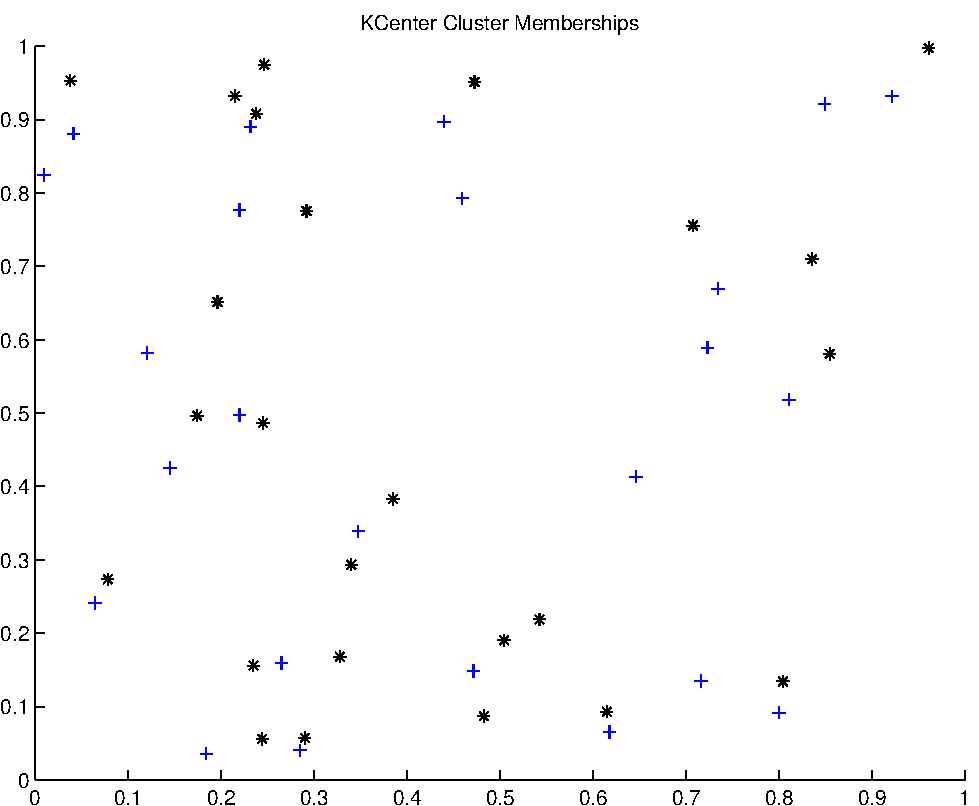
\includegraphics[width=10.0cm,height=10.0cm]{KCenterClusterMemberships_25_Centers.pdf}

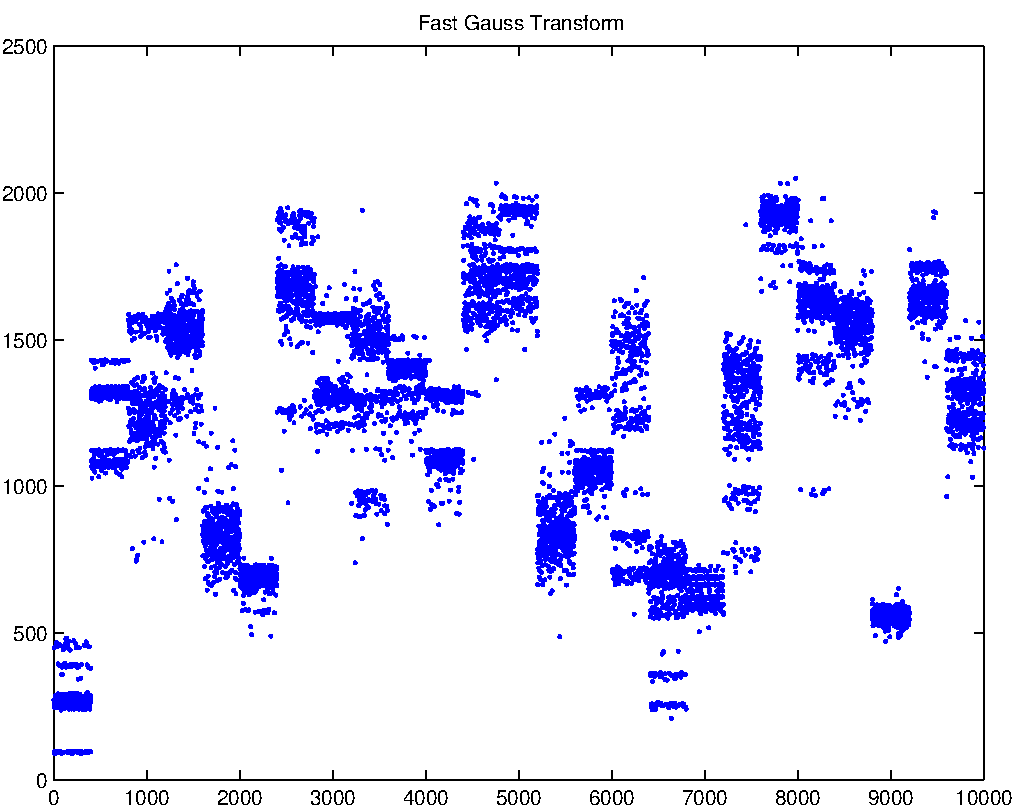
\includegraphics[width=10.0cm,height=10.0cm]{FGT25_Centers.pdf}

QueryPerformanceCounter  =  +7.514
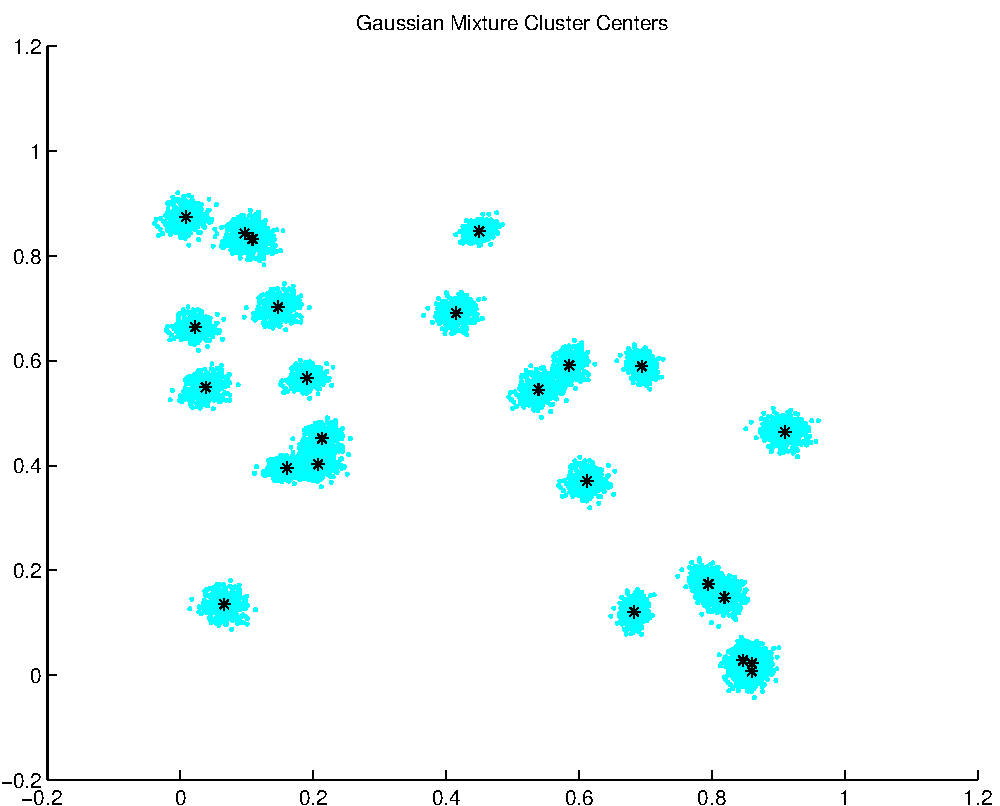
\includegraphics[width=10.0cm,height=10.0cm]{GaussianMixture_ClusterCenters24_Centers.pdf}

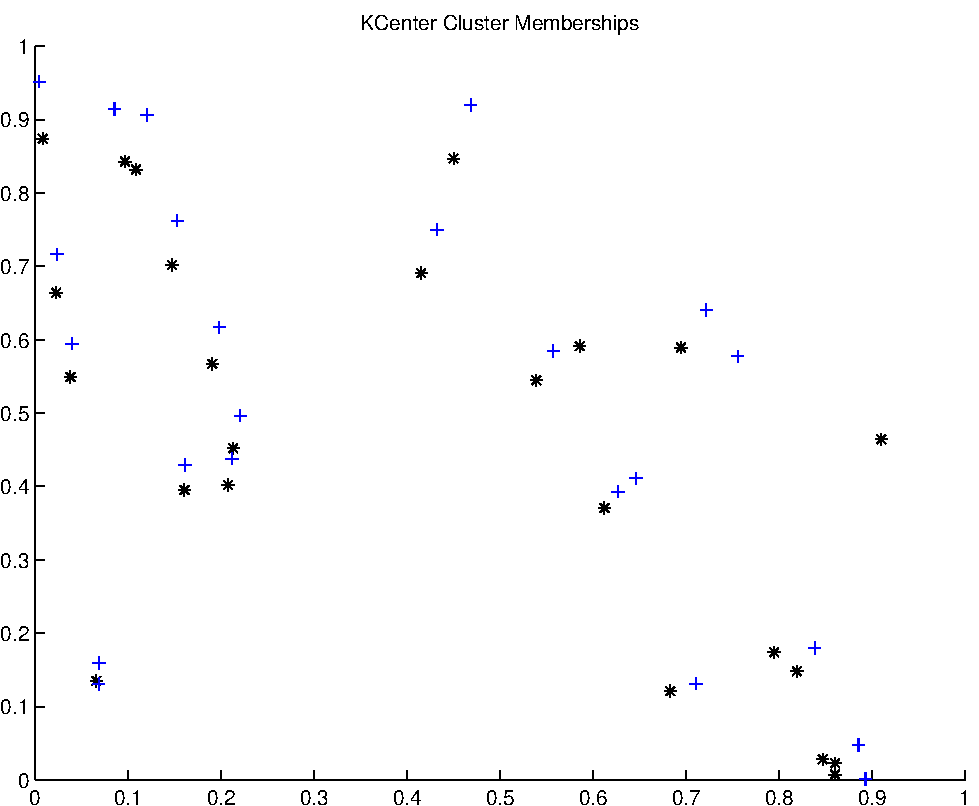
\includegraphics[width=10.0cm,height=10.0cm]{KCenterClusterMemberships_24_Centers.pdf}

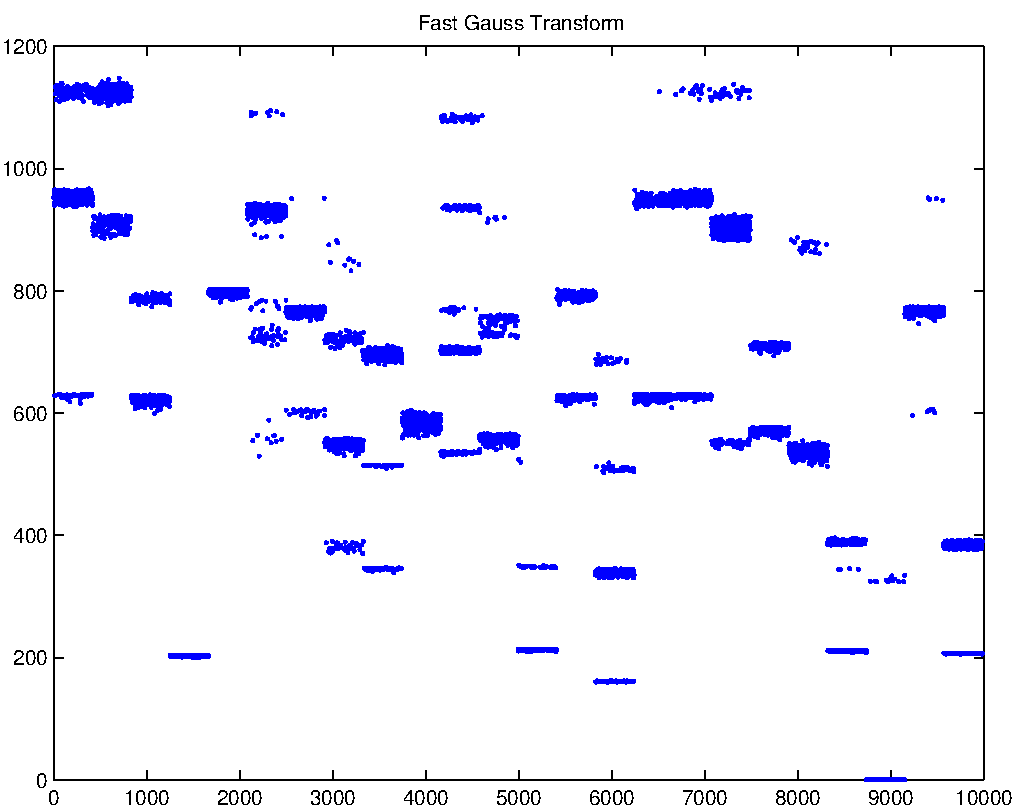
\includegraphics[width=10.0cm,height=10.0cm]{FGT24_Centers.pdf}

QueryPerformanceCounter  =  +7.976
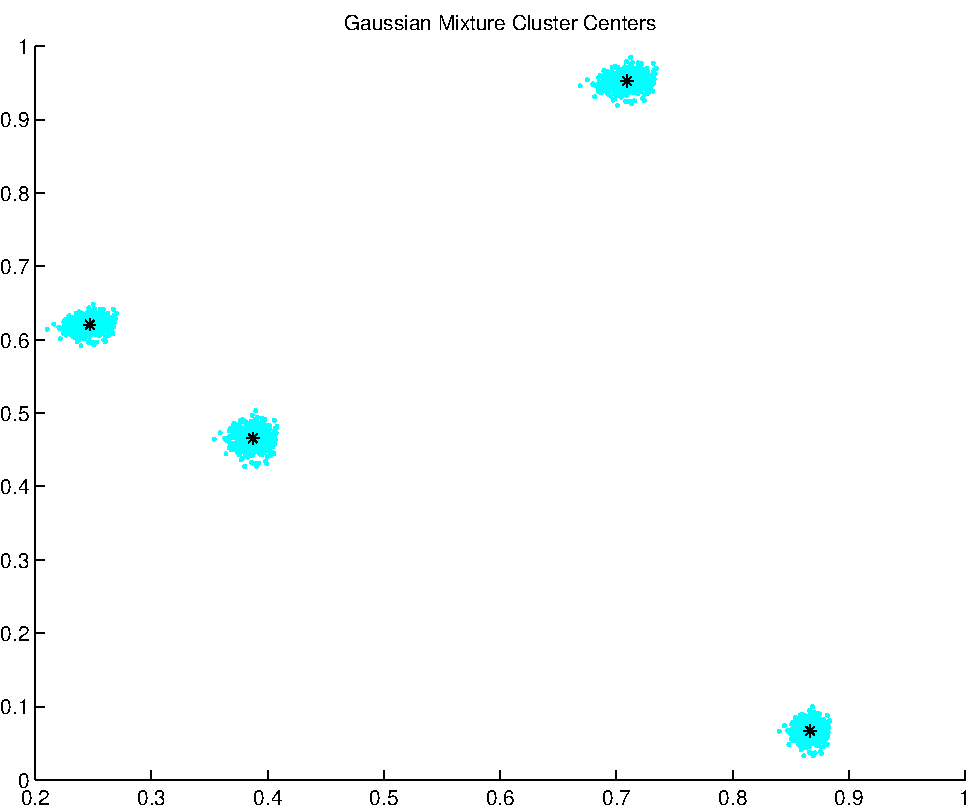
\includegraphics[width=10.0cm,height=10.0cm]{GaussianMixture_ClusterCenters4_Centers.pdf}

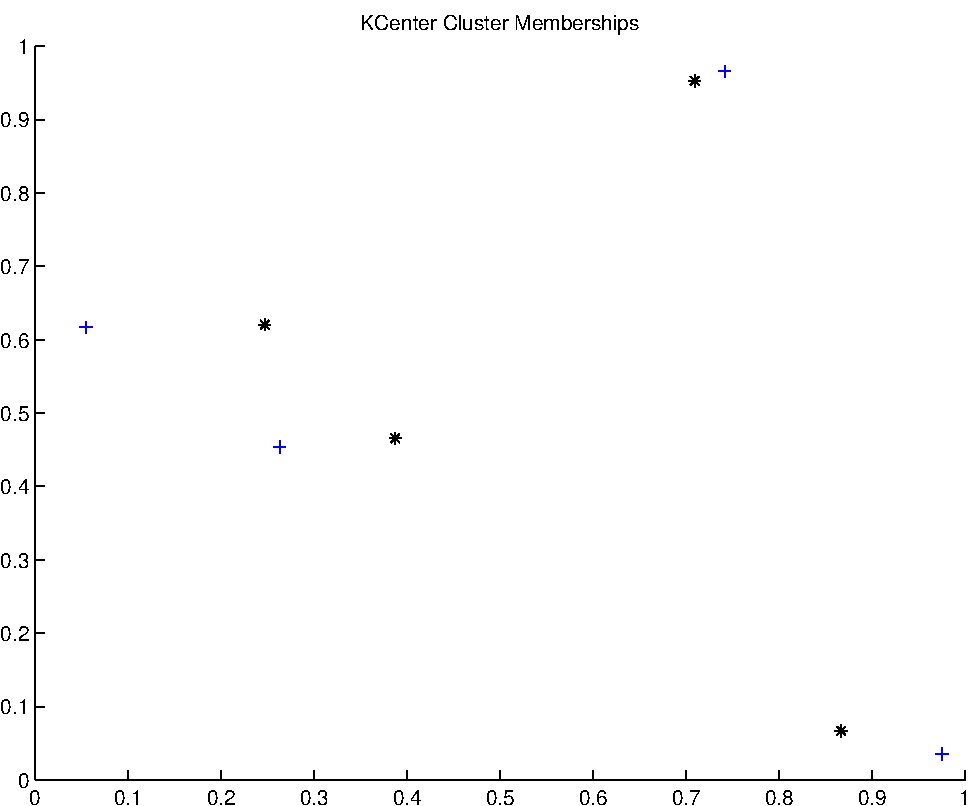
\includegraphics[width=10.0cm,height=10.0cm]{KCenterClusterMemberships_4_Centers.pdf}

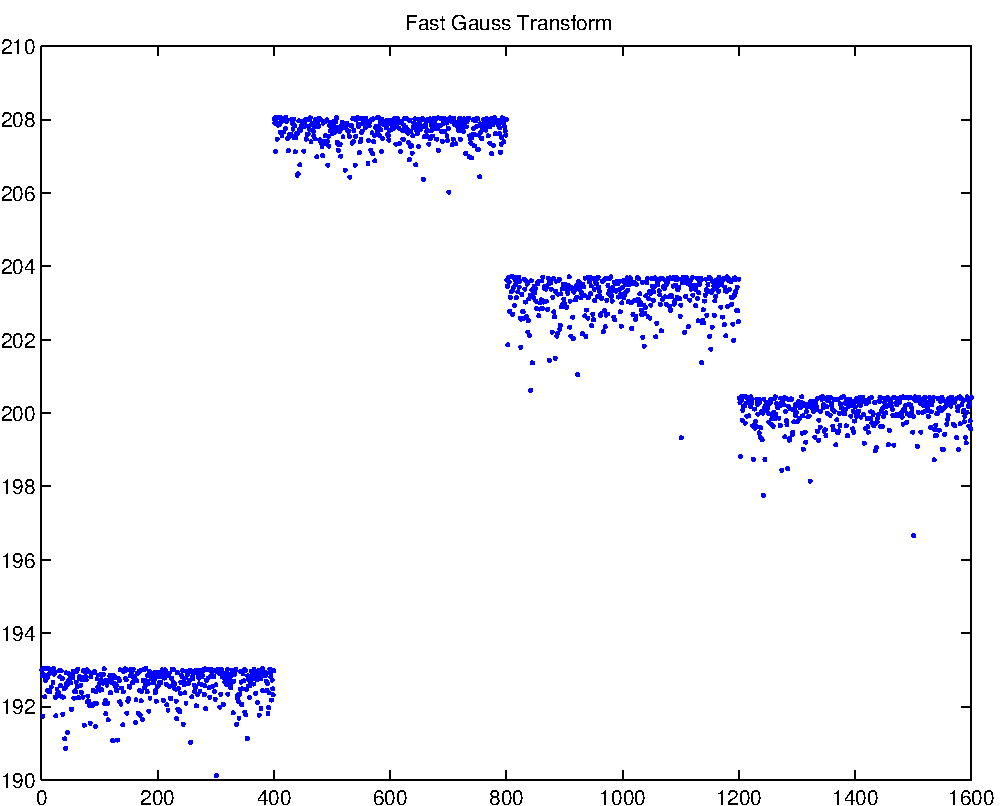
\includegraphics[width=10.0cm,height=10.0cm]{FGT4_Centers.pdf}

QueryPerformanceCounter  =  +3.950
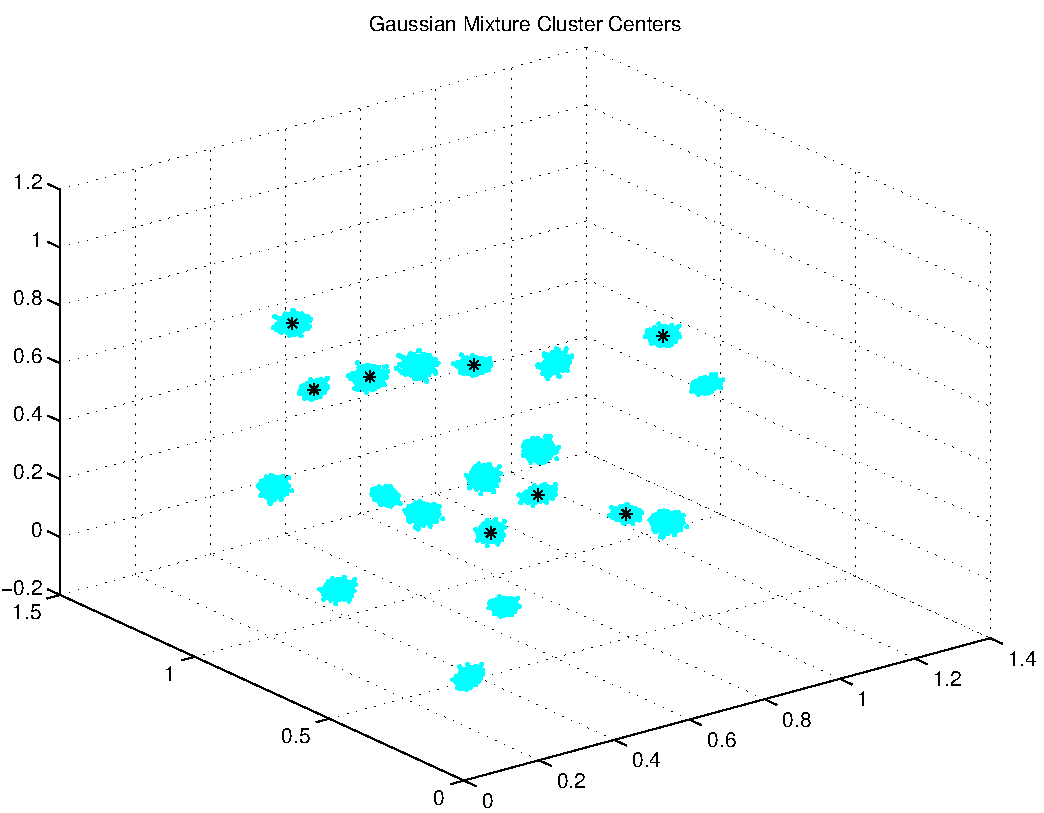
\includegraphics[width=10.0cm,height=10.0cm]{GaussianMixture_ClusterCenters20_Centers.pdf}

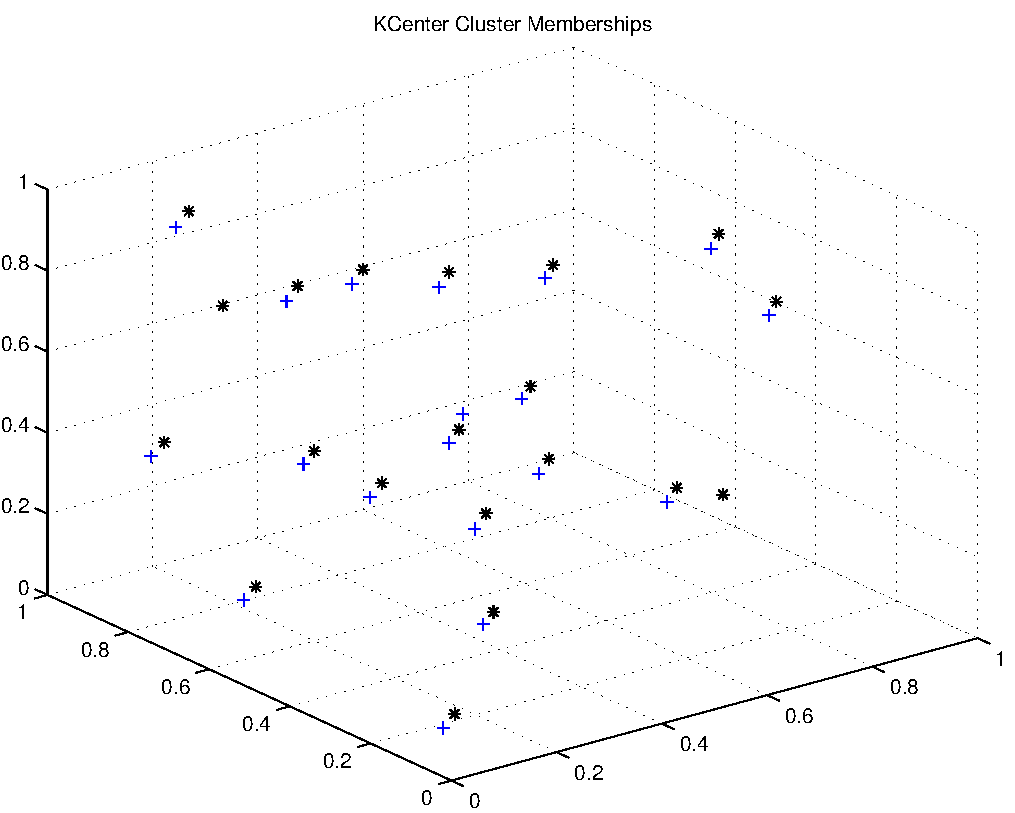
\includegraphics[width=10.0cm,height=10.0cm]{KCenterClusterMemberships_20_Centers.pdf}

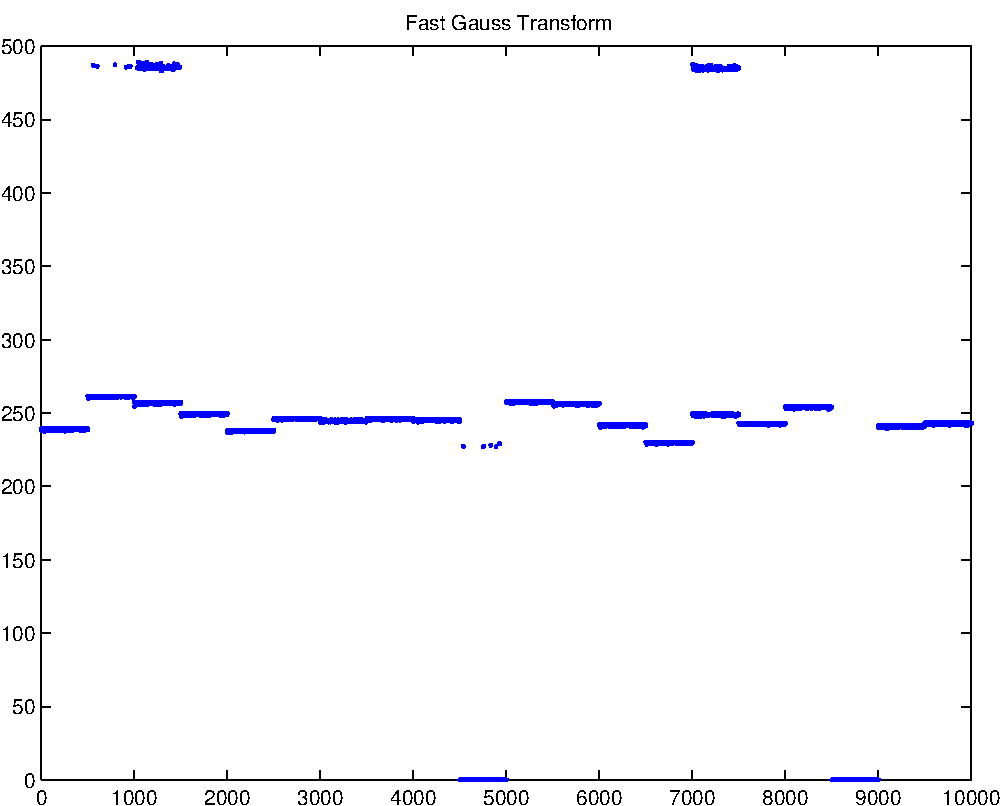
\includegraphics[width=10.0cm,height=10.0cm]{FGT20_Centers.pdf}

QueryPerformanceCounter  =  +6.765
\subsubsection{Matrix Norms}
\subsubsection{Haar Distributed Random Orthogonal Matrix $A \in O(n)$}
 Testing Operator Norm
Number of Dimensions: +12

$A = \left(
\begin{array}{
cccccccccccc}
-0.198 & -0.070 & +0.207 & +0.158 & +0.267 & -0.636 & -0.018 & +0.246 & +0.107 & +0.193 & -0.205 & +0.510 \\
+0.175 & +0.037 & -0.071 & -0.376 & -0.348 & +0.304 & +0.223 & +0.138 & -0.231 & +0.085 & -0.350 & +0.597 \\
+0.374 & -0.046 & -0.111 & +0.280 & +0.523 & +0.467 & -0.233 & -0.091 & +0.253 & +0.250 & +0.002 & +0.295 \\
+0.232 & -0.093 & +0.222 & +0.338 & -0.523 & -0.145 & -0.227 & -0.491 & +0.093 & -0.156 & +0.214 & +0.328 \\
-0.262 & +0.129 & -0.551 & +0.105 & -0.286 & -0.007 & -0.561 & +0.302 & -0.093 & +0.230 & +0.203 & +0.097 \\
-0.636 & +0.357 & +0.418 & +0.026 & +0.040 & +0.373 & +0.045 & -0.177 & -0.026 & +0.180 & +0.225 & +0.184 \\
-0.069 & -0.193 & +0.131 & +0.004 & -0.385 & +0.106 & +0.065 & +0.118 & +0.653 & +0.460 & -0.256 & -0.243 \\
-0.114 & -0.573 & -0.163 & +0.290 & -0.033 & +0.054 & +0.459 & -0.024 & -0.327 & +0.348 & +0.322 & +0.032 \\
+0.030 & -0.458 & +0.312 & -0.592 & +0.106 & -0.025 & -0.468 & -0.093 & -0.153 & +0.214 & +0.178 & -0.030 \\
+0.251 & -0.001 & +0.395 & +0.112 & -0.104 & +0.147 & +0.023 & +0.713 & +0.049 & -0.196 & +0.430 & +0.034 \\
+0.028 & -0.048 & +0.326 & +0.421 & -0.073 & +0.139 & -0.278 & +0.103 & -0.507 & +0.106 & -0.520 & -0.250 \\
-0.424 & -0.511 & -0.088 & +0.073 & +0.036 & +0.262 & -0.122 & +0.081 & +0.192 & -0.596 & -0.205 & +0.146 \\
\end{array}
\right)$ \newline 

$Det(A) :   A \in O(n)$ = (-1.000,+0.000)

$L = \left(
\begin{array}{
cccccccccccc}
+1.000 & +0.000 & +0.000 & +0.000 & +0.000 & +0.000 & +0.000 & +0.000 & +0.000 & +0.000 & +0.000 & +0.000 \\
+0.666 & +1.000 & +0.000 & +0.000 & +0.000 & +0.000 & +0.000 & +0.000 & +0.000 & +0.000 & +0.000 & +0.000 \\
+0.412 & +0.025 & +1.000 & +0.000 & +0.000 & +0.000 & +0.000 & +0.000 & +0.000 & +0.000 & +0.000 & +0.000 \\
-0.047 & +0.589 & -0.767 & +1.000 & +0.000 & +0.000 & +0.000 & +0.000 & +0.000 & +0.000 & +0.000 & +0.000 \\
-0.365 & -0.050 & -0.499 & -0.720 & +1.000 & +0.000 & +0.000 & +0.000 & +0.000 & +0.000 & +0.000 & +0.000 \\
+0.311 & +0.242 & -0.232 & -0.286 & -0.192 & +1.000 & +0.000 & +0.000 & +0.000 & +0.000 & +0.000 & +0.000 \\
-0.588 & -0.219 & -0.077 & -0.570 & -0.599 & -0.559 & +1.000 & +0.000 & +0.000 & +0.000 & +0.000 & +0.000 \\
-0.395 & -0.187 & -0.689 & -0.356 & +0.453 & -0.256 & +0.189 & +1.000 & +0.000 & +0.000 & +0.000 & +0.000 \\
-0.044 & +0.043 & -0.504 & -0.846 & +0.444 & -0.046 & +0.459 & +0.443 & +1.000 & +0.000 & +0.000 & +0.000 \\
+0.179 & +0.851 & -0.104 & -0.448 & +0.184 & +0.078 & -0.232 & -0.070 & +0.895 & +1.000 & +0.000 & +0.000 \\
+0.109 & +0.309 & -0.278 & -0.019 & +0.637 & -0.154 & -0.313 & +0.328 & -0.908 & +0.854 & +1.000 & +0.000 \\
-0.276 & -0.181 & +0.031 & +0.656 & +0.319 & -0.651 & -0.428 & +0.266 & +0.001 & +0.294 & +0.406 & +1.000 \\
\end{array}
\right)$ \newline 

$U = \left(
\begin{array}{
cccccccccccc}
-0.636 & +0.357 & +0.418 & +0.026 & +0.040 & +0.373 & +0.045 & -0.177 & -0.026 & +0.180 & +0.225 & +0.184 \\
+0.000 & -0.749 & -0.367 & +0.056 & +0.010 & +0.013 & -0.153 & +0.198 & +0.209 & -0.716 & -0.354 & +0.023 \\
+0.000 & +0.000 & -0.715 & +0.093 & -0.303 & -0.161 & -0.576 & +0.370 & -0.088 & +0.174 & +0.119 & +0.021 \\
+0.000 & +0.000 & +0.000 & -0.552 & -0.131 & -0.138 & -0.818 & +0.065 & -0.344 & +0.778 & +0.489 & -0.020 \\
+0.000 & +0.000 & +0.000 & +0.000 & -0.753 & -0.188 & -1.094 & -0.314 & -0.198 & +0.521 & +0.690 & +0.393 \\
+0.000 & +0.000 & +0.000 & +0.000 & +0.000 & -0.869 & -0.573 & +0.297 & -0.093 & +0.673 & +0.111 & +0.522 \\
+0.000 & +0.000 & +0.000 & +0.000 & +0.000 & +0.000 & -1.726 & -0.108 & -0.090 & +1.343 & +0.820 & +0.926 \\
+0.000 & +0.000 & +0.000 & +0.000 & +0.000 & +0.000 & +0.000 & +1.197 & -0.022 & -0.179 & +0.270 & -0.102 \\
+0.000 & +0.000 & +0.000 & +0.000 & +0.000 & +0.000 & +0.000 & +0.000 & -0.718 & +0.153 & -0.818 & -0.779 \\
+0.000 & +0.000 & +0.000 & +0.000 & +0.000 & +0.000 & +0.000 & +0.000 & +0.000 & +1.306 & +1.620 & +0.764 \\
+0.000 & +0.000 & +0.000 & +0.000 & +0.000 & +0.000 & +0.000 & +0.000 & +0.000 & +0.000 & -2.509 & -1.471 \\
+0.000 & +0.000 & +0.000 & +0.000 & +0.000 & +0.000 & +0.000 & +0.000 & +0.000 & +0.000 & +0.000 & +1.676 \\
\end{array}
\right)$ \newline 

$L * U  = \left(
\begin{array}{
cccccccccccc}
-0.636 & +0.357 & +0.418 & +0.026 & +0.040 & +0.373 & +0.045 & -0.177 & -0.026 & +0.180 & +0.225 & +0.184 \\
-0.424 & -0.511 & -0.088 & +0.073 & +0.036 & +0.262 & -0.122 & +0.081 & +0.192 & -0.596 & -0.205 & +0.146 \\
-0.262 & +0.129 & -0.551 & +0.105 & -0.286 & -0.007 & -0.561 & +0.302 & -0.093 & +0.230 & +0.203 & +0.097 \\
+0.030 & -0.458 & +0.312 & -0.592 & +0.106 & -0.025 & -0.468 & -0.093 & -0.153 & +0.214 & +0.178 & -0.030 \\
+0.232 & -0.093 & +0.222 & +0.338 & -0.523 & -0.145 & -0.227 & -0.491 & +0.093 & -0.156 & +0.214 & +0.328 \\
-0.198 & -0.070 & +0.207 & +0.158 & +0.267 & -0.636 & -0.018 & +0.246 & +0.107 & +0.193 & -0.205 & +0.510 \\
+0.374 & -0.046 & -0.111 & +0.280 & +0.523 & +0.467 & -0.233 & -0.091 & +0.253 & +0.250 & +0.002 & +0.295 \\
+0.251 & -0.001 & +0.395 & +0.112 & -0.104 & +0.147 & +0.023 & +0.713 & +0.049 & -0.196 & +0.430 & +0.034 \\
+0.028 & -0.048 & +0.326 & +0.421 & -0.073 & +0.139 & -0.278 & +0.103 & -0.507 & +0.106 & -0.520 & -0.250 \\
-0.114 & -0.573 & -0.163 & +0.290 & -0.033 & +0.054 & +0.459 & -0.024 & -0.327 & +0.348 & +0.322 & +0.032 \\
-0.069 & -0.193 & +0.131 & +0.004 & -0.385 & +0.106 & +0.065 & +0.118 & +0.653 & +0.460 & -0.256 & -0.243 \\
+0.175 & +0.037 & -0.071 & -0.376 & -0.348 & +0.304 & +0.223 & +0.138 & -0.231 & +0.085 & -0.350 & +0.597 \\
\end{array}
\right)$ \newline 

$Det(L) :    = (+1.000,+0.000)     Det(U) :    = (-1.000,+0.000)     Det(LU) :    = (-1.000,+0.000)$

$||A||_{L_1}$  = +3.109

$||A||_{L_{\infty}}$ = +3.063

$||A^{-1}||_{L_1}$  = +3.063

$||A^{-1}||_{L_{\infty}}$ = +3.109

$||A||_{L_{\infty}} * ||A^{-1}||_{L_{\infty}} = +9.524$

$||A||_{L_1} * ||A^{-1}||_{L_1} = +9.524$

Frobenious Norm  $||A||_{\textit{F}}$ via $\sum\limits_{i,j =0}^{n} \|A_{i,j}|$   of  $A \in O(n)$  +3.464

$L_1$ condition number of Haar Distributed Random Orthogonal Matrix $A \in O(n)$ +8.345

$A = \left(
\begin{array}{
cccccccccccc}
-0.198 & -0.070 & +0.207 & +0.158 & +0.267 & -0.636 & -0.018 & +0.246 & +0.107 & +0.193 & -0.205 & +0.510 \\
+0.175 & +0.037 & -0.071 & -0.376 & -0.348 & +0.304 & +0.223 & +0.138 & -0.231 & +0.085 & -0.350 & +0.597 \\
+0.374 & -0.046 & -0.111 & +0.280 & +0.523 & +0.467 & -0.233 & -0.091 & +0.253 & +0.250 & +0.002 & +0.295 \\
+0.232 & -0.093 & +0.222 & +0.338 & -0.523 & -0.145 & -0.227 & -0.491 & +0.093 & -0.156 & +0.214 & +0.328 \\
-0.262 & +0.129 & -0.551 & +0.105 & -0.286 & -0.007 & -0.561 & +0.302 & -0.093 & +0.230 & +0.203 & +0.097 \\
-0.636 & +0.357 & +0.418 & +0.026 & +0.040 & +0.373 & +0.045 & -0.177 & -0.026 & +0.180 & +0.225 & +0.184 \\
-0.069 & -0.193 & +0.131 & +0.004 & -0.385 & +0.106 & +0.065 & +0.118 & +0.653 & +0.460 & -0.256 & -0.243 \\
-0.114 & -0.573 & -0.163 & +0.290 & -0.033 & +0.054 & +0.459 & -0.024 & -0.327 & +0.348 & +0.322 & +0.032 \\
+0.030 & -0.458 & +0.312 & -0.592 & +0.106 & -0.025 & -0.468 & -0.093 & -0.153 & +0.214 & +0.178 & -0.030 \\
+0.251 & -0.001 & +0.395 & +0.112 & -0.104 & +0.147 & +0.023 & +0.713 & +0.049 & -0.196 & +0.430 & +0.034 \\
+0.028 & -0.048 & +0.326 & +0.421 & -0.073 & +0.139 & -0.278 & +0.103 & -0.507 & +0.106 & -0.520 & -0.250 \\
-0.424 & -0.511 & -0.088 & +0.073 & +0.036 & +0.262 & -0.122 & +0.081 & +0.192 & -0.596 & -0.205 & +0.146 \\
\end{array}
\right)$ \newline 

$L_{\infty}$ condition number of Haar Distributed Random Orthogonal Matrix $A \in O(n)$ +8.341

Eigenvalues of $A \in O(n)$

(+0.176,+0.984), (+0.176,-0.984), (+0.406,+0.914), (+0.406,-0.914), (-0.698,+0.716), (-0.698,-0.716), (-0.995,+0.096), (-0.995,-0.096), (-1.000,+0.000), (+1.000,+0.000), (+0.848,+0.531), (+0.848,-0.531)

 $|\lambda | : \lambda \in \sigma(A) , A \in O(n)$

+1.000, +1.000, +1.000, +1.000, +1.000, +1.000, +1.000, +1.000, +1.000, +1.000, +1.000, +1.000


Calculating $A^{\dag} A,$  we expect $A^{\dag} A \approx I$

$A^{\dag} A = \left(
\begin{array}{
cccccccccccc}
+1.000 & +0.000 & -0.000 & +0.000 & +0.000 & -0.000 & -0.000 & +0.000 & -0.000 & +0.000 & -0.000 & +0.000 \\
+0.000 & +1.000 & -0.000 & +0.000 & -0.000 & -0.000 & +0.000 & -0.000 & -0.000 & +0.000 & -0.000 & +0.000 \\
-0.000 & -0.000 & +1.000 & +0.000 & +0.000 & +0.000 & -0.000 & -0.000 & -0.000 & -0.000 & -0.000 & -0.000 \\
+0.000 & +0.000 & +0.000 & +1.000 & -0.000 & +0.000 & +0.000 & +0.000 & +0.000 & +0.000 & -0.000 & -0.000 \\
+0.000 & -0.000 & +0.000 & -0.000 & +1.000 & -0.000 & -0.000 & -0.000 & +0.000 & -0.000 & +0.000 & +0.000 \\
-0.000 & -0.000 & +0.000 & +0.000 & -0.000 & +1.000 & +0.000 & +0.000 & +0.000 & -0.000 & -0.000 & +0.000 \\
-0.000 & +0.000 & -0.000 & +0.000 & -0.000 & +0.000 & +1.000 & -0.000 & +0.000 & +0.000 & +0.000 & +0.000 \\
+0.000 & -0.000 & -0.000 & +0.000 & -0.000 & +0.000 & -0.000 & +1.000 & -0.000 & -0.000 & -0.000 & -0.000 \\
-0.000 & -0.000 & -0.000 & +0.000 & +0.000 & +0.000 & +0.000 & -0.000 & +1.000 & +0.000 & +0.000 & -0.000 \\
+0.000 & +0.000 & -0.000 & +0.000 & -0.000 & -0.000 & +0.000 & -0.000 & +0.000 & +1.000 & -0.000 & -0.000 \\
-0.000 & -0.000 & -0.000 & -0.000 & +0.000 & -0.000 & +0.000 & -0.000 & +0.000 & -0.000 & +1.000 & +0.000 \\
+0.000 & +0.000 & -0.000 & -0.000 & +0.000 & +0.000 & +0.000 & -0.000 & -0.000 & -0.000 & +0.000 & +1.000 \\
\end{array}
\right)$ \newline 

Calculating $A^{-1} ,  A \in O(n)$.

$A^{-1} = \left(
\begin{array}{
cccccccccccc}
-0.198 & +0.175 & +0.374 & +0.232 & -0.262 & -0.636 & -0.069 & -0.114 & +0.030 & +0.251 & +0.028 & -0.424 \\
-0.070 & +0.037 & -0.046 & -0.093 & +0.129 & +0.357 & -0.193 & -0.573 & -0.458 & -0.001 & -0.048 & -0.511 \\
+0.207 & -0.071 & -0.111 & +0.222 & -0.551 & +0.418 & +0.131 & -0.163 & +0.312 & +0.395 & +0.326 & -0.088 \\
+0.158 & -0.376 & +0.280 & +0.338 & +0.105 & +0.026 & +0.004 & +0.290 & -0.592 & +0.112 & +0.421 & +0.073 \\
+0.267 & -0.348 & +0.523 & -0.523 & -0.286 & +0.040 & -0.385 & -0.033 & +0.106 & -0.104 & -0.073 & +0.036 \\
-0.636 & +0.304 & +0.467 & -0.145 & -0.007 & +0.373 & +0.106 & +0.054 & -0.025 & +0.147 & +0.139 & +0.262 \\
-0.018 & +0.223 & -0.233 & -0.227 & -0.561 & +0.045 & +0.065 & +0.459 & -0.468 & +0.023 & -0.278 & -0.122 \\
+0.246 & +0.138 & -0.091 & -0.491 & +0.302 & -0.177 & +0.118 & -0.024 & -0.093 & +0.713 & +0.103 & +0.081 \\
+0.107 & -0.231 & +0.253 & +0.093 & -0.093 & -0.026 & +0.653 & -0.327 & -0.153 & +0.049 & -0.507 & +0.192 \\
+0.193 & +0.085 & +0.250 & -0.156 & +0.230 & +0.180 & +0.460 & +0.348 & +0.214 & -0.196 & +0.106 & -0.596 \\
-0.205 & -0.350 & +0.002 & +0.214 & +0.203 & +0.225 & -0.256 & +0.322 & +0.178 & +0.430 & -0.520 & -0.205 \\
+0.510 & +0.597 & +0.295 & +0.328 & +0.097 & +0.184 & -0.243 & +0.032 & -0.030 & +0.034 & -0.250 & +0.146 \\
\end{array}
\right)$ \newline 

Calculating $A^{-1} *A  ,  A \in O(n)$.   We expect $A^{-1} *A  \approx I$. 

$A^{-1} *A = \left(
\begin{array}{
cccccccccccc}
+1.000 & +0.000 & +0.000 & +0.000 & +0.000 & +0.000 & +0.000 & -0.000 & -0.000 & +0.000 & +0.000 & +0.000 \\
+0.000 & +1.000 & +0.000 & +0.000 & -0.000 & +0.000 & -0.000 & +0.000 & -0.000 & +0.000 & -0.000 & +0.000 \\
-0.000 & +0.000 & +1.000 & +0.000 & +0.000 & -0.000 & -0.000 & +0.000 & -0.000 & -0.000 & -0.000 & -0.000 \\
-0.000 & +0.000 & -0.000 & +1.000 & +0.000 & +0.000 & +0.000 & +0.000 & -0.000 & -0.000 & -0.000 & -0.000 \\
-0.000 & +0.000 & +0.000 & +0.000 & +1.000 & +0.000 & -0.000 & +0.000 & +0.000 & +0.000 & +0.000 & +0.000 \\
-0.000 & +0.000 & +0.000 & +0.000 & +0.000 & +1.000 & +0.000 & -0.000 & -0.000 & -0.000 & -0.000 & -0.000 \\
-0.000 & +0.000 & -0.000 & -0.000 & -0.000 & -0.000 & +1.000 & +0.000 & +0.000 & +0.000 & +0.000 & +0.000 \\
+0.000 & +0.000 & -0.000 & +0.000 & -0.000 & -0.000 & +0.000 & +1.000 & +0.000 & -0.000 & -0.000 & -0.000 \\
-0.000 & -0.000 & +0.000 & -0.000 & +0.000 & +0.000 & -0.000 & -0.000 & +1.000 & +0.000 & -0.000 & +0.000 \\
+0.000 & -0.000 & +0.000 & +0.000 & -0.000 & +0.000 & -0.000 & -0.000 & -0.000 & +1.000 & +0.000 & +0.000 \\
+0.000 & -0.000 & +0.000 & +0.000 & +0.000 & -0.000 & +0.000 & +0.000 & +0.000 & +0.000 & +1.000 & -0.000 \\
-0.000 & +0.000 & -0.000 & -0.000 & +0.000 & +0.000 & +0.000 & +0.000 & +0.000 & +0.000 & +0.000 & +1.000 \\
\end{array}
\right)$ \newline 

Calculating SVD of  $A \in O(n)$

$U = \left(
\begin{array}{
cccccccccccc}
+0.062 & +0.310 & +0.304 & +0.585 & -0.153 & +0.188 & +0.024 & +0.049 & +0.117 & -0.321 & -0.532 & -0.064 \\
+0.040 & +0.520 & -0.091 & +0.011 & -0.164 & -0.013 & +0.406 & +0.235 & +0.510 & +0.390 & +0.236 & -0.068 \\
+0.113 & +0.534 & +0.156 & -0.398 & +0.397 & -0.019 & -0.210 & +0.423 & -0.280 & -0.177 & -0.051 & -0.160 \\
+0.110 & -0.306 & +0.004 & +0.059 & +0.701 & +0.472 & +0.269 & +0.121 & +0.282 & +0.041 & -0.078 & +0.048 \\
-0.198 & -0.070 & +0.207 & +0.158 & +0.267 & -0.636 & -0.018 & +0.246 & +0.107 & +0.193 & -0.205 & +0.510 \\
-0.064 & +0.315 & -0.409 & +0.280 & +0.192 & +0.233 & -0.602 & -0.194 & +0.024 & +0.314 & +0.019 & +0.245 \\
-0.035 & +0.300 & -0.244 & +0.190 & +0.279 & -0.200 & +0.369 & -0.364 & -0.126 & -0.509 & +0.327 & +0.212 \\
-0.033 & +0.037 & -0.327 & +0.114 & -0.064 & +0.119 & +0.440 & +0.181 & -0.650 & +0.334 & -0.302 & +0.088 \\
+0.230 & -0.033 & +0.504 & +0.377 & -0.023 & +0.157 & -0.044 & +0.138 & -0.324 & +0.177 & +0.589 & +0.141 \\
+0.899 & -0.077 & -0.211 & +0.087 & +0.038 & -0.321 & -0.050 & -0.053 & +0.035 & +0.060 & -0.116 & -0.076 \\
+0.059 & +0.217 & +0.446 & -0.241 & +0.152 & +0.001 & +0.141 & -0.679 & -0.077 & +0.370 & -0.214 & -0.009 \\
-0.243 & -0.063 & -0.039 & +0.368 & +0.293 & -0.317 & -0.034 & -0.046 & -0.073 & +0.184 & +0.078 & -0.751 \\
\end{array}
\right)$ \newline 

$S = \left(
\begin{array}{
cccccccccccc}
+1.000 & +0.000 & +0.000 & +0.000 & +0.000 & +0.000 & +0.000 & +0.000 & +0.000 & +0.000 & +0.000 & +0.000 \\
+0.000 & +1.000 & +0.000 & +0.000 & +0.000 & +0.000 & +0.000 & +0.000 & +0.000 & +0.000 & +0.000 & +0.000 \\
+0.000 & +0.000 & +1.000 & +0.000 & +0.000 & +0.000 & +0.000 & +0.000 & +0.000 & +0.000 & +0.000 & +0.000 \\
+0.000 & +0.000 & +0.000 & +1.000 & +0.000 & +0.000 & +0.000 & +0.000 & +0.000 & +0.000 & +0.000 & +0.000 \\
+0.000 & +0.000 & +0.000 & +0.000 & +1.000 & +0.000 & +0.000 & +0.000 & +0.000 & +0.000 & +0.000 & +0.000 \\
+0.000 & +0.000 & +0.000 & +0.000 & +0.000 & +1.000 & +0.000 & +0.000 & +0.000 & +0.000 & +0.000 & +0.000 \\
+0.000 & +0.000 & +0.000 & +0.000 & +0.000 & +0.000 & +1.000 & +0.000 & +0.000 & +0.000 & +0.000 & +0.000 \\
+0.000 & +0.000 & +0.000 & +0.000 & +0.000 & +0.000 & +0.000 & +1.000 & +0.000 & +0.000 & +0.000 & +0.000 \\
+0.000 & +0.000 & +0.000 & +0.000 & +0.000 & +0.000 & +0.000 & +0.000 & +1.000 & +0.000 & +0.000 & +0.000 \\
+0.000 & +0.000 & +0.000 & +0.000 & +0.000 & +0.000 & +0.000 & +0.000 & +0.000 & +1.000 & +0.000 & +0.000 \\
+0.000 & +0.000 & +0.000 & +0.000 & +0.000 & +0.000 & +0.000 & +0.000 & +0.000 & +0.000 & +1.000 & +0.000 \\
+0.000 & +0.000 & +0.000 & +0.000 & +0.000 & +0.000 & +0.000 & +0.000 & +0.000 & +0.000 & +0.000 & +1.000 \\
\end{array}
\right)$ \newline 

$V = \left(
\begin{array}{
cccccccccccc}
-0.000 & -0.000 & +0.000 & +0.000 & +1.000 & +0.000 & +0.000 & +0.000 & -0.000 & -0.000 & -0.000 & -0.000 \\
-0.003 & -0.003 & +0.018 & -0.044 & +0.000 & -0.072 & -0.177 & +0.494 & -0.105 & +0.000 & +0.082 & -0.836 \\
+0.066 & +0.003 & -0.064 & +0.680 & +0.000 & +0.609 & -0.043 & -0.099 & +0.201 & +0.276 & +0.074 & -0.157 \\
+0.201 & -0.161 & -0.550 & -0.461 & +0.000 & +0.095 & +0.160 & -0.366 & +0.342 & +0.207 & +0.120 & -0.277 \\
-0.237 & +0.082 & +0.003 & -0.410 & +0.000 & +0.633 & -0.212 & +0.116 & -0.027 & -0.138 & -0.538 & +0.032 \\
+0.078 & +0.186 & +0.033 & +0.011 & +0.000 & +0.197 & +0.074 & -0.045 & +0.292 & -0.827 & +0.373 & -0.060 \\
+0.145 & +0.469 & -0.423 & +0.075 & +0.000 & -0.124 & -0.686 & -0.175 & -0.219 & -0.034 & +0.058 & +0.071 \\
-0.363 & -0.057 & -0.572 & +0.201 & +0.000 & -0.176 & +0.061 & +0.510 & +0.367 & -0.069 & -0.113 & +0.225 \\
-0.607 & -0.452 & +0.145 & -0.015 & +0.000 & -0.065 & -0.469 & -0.306 & +0.145 & -0.026 & +0.250 & -0.062 \\
+0.117 & +0.214 & +0.291 & +0.100 & +0.000 & -0.328 & -0.153 & -0.186 & +0.630 & +0.000 & -0.502 & -0.178 \\
+0.567 & -0.450 & +0.121 & -0.114 & +0.000 & +0.084 & -0.416 & +0.356 & +0.223 & +0.026 & +0.107 & +0.281 \\
+0.189 & -0.507 & -0.255 & +0.292 & +0.000 & -0.102 & +0.024 & -0.227 & -0.309 & -0.414 & -0.451 & -0.155 \\
\end{array}
\right)$ \newline 

$U S V = \left(
\begin{array}{
cccccccccccc}
-0.249 & +0.087 & -0.492 & +0.008 & +0.062 & +0.207 & +0.272 & -0.248 & +0.016 & +0.076 & +0.427 & -0.563 \\
-0.137 & -0.060 & -0.065 & +0.040 & +0.040 & -0.424 & -0.715 & +0.163 & +0.322 & +0.001 & +0.106 & -0.371 \\
-0.261 & +0.162 & +0.009 & +0.118 & +0.113 & +0.307 & +0.096 & +0.830 & -0.090 & -0.029 & -0.188 & -0.208 \\
-0.322 & +0.147 & -0.173 & -0.226 & +0.110 & +0.469 & -0.332 & -0.231 & +0.193 & -0.521 & -0.197 & +0.225 \\
-0.222 & -0.317 & -0.338 & +0.193 & -0.198 & +0.009 & -0.030 & -0.182 & -0.062 & +0.344 & -0.703 & -0.095 \\
+0.063 & -0.336 & +0.287 & -0.481 & -0.064 & -0.098 & +0.323 & -0.002 & +0.234 & -0.342 & -0.261 & -0.461 \\
+0.367 & -0.159 & -0.219 & -0.453 & -0.035 & +0.185 & -0.356 & +0.095 & -0.627 & +0.035 & +0.031 & -0.143 \\
+0.303 & +0.650 & -0.383 & -0.076 & -0.033 & -0.396 & +0.140 & +0.020 & -0.003 & -0.211 & -0.326 & -0.066 \\
+0.649 & -0.212 & -0.256 & +0.202 & +0.230 & +0.341 & -0.017 & +0.108 & +0.493 & +0.047 & -0.038 & -0.007 \\
-0.113 & -0.003 & +0.033 & -0.217 & +0.899 & -0.162 & +0.057 & -0.095 & -0.068 & +0.253 & -0.148 & +0.045 \\
+0.179 & +0.372 & +0.510 & +0.276 & +0.059 & +0.298 & -0.198 & -0.322 & -0.123 & +0.093 & -0.198 & -0.443 \\
-0.043 & +0.311 & +0.075 & -0.538 & -0.243 & +0.179 & -0.038 & +0.055 & +0.370 & +0.606 & +0.000 & +0.083 \\
\end{array}
\right)$ \newline 

\subsubsection{Wishart Matrix $A \in W(n)$}
$L_1$ condition number of Wishart Matrix +56267.800
$L_infty$ condition number of Wishart Matrix +56267.800
\subsubsection{Gaussian Orthogonal Ensemble $A \in GOE(n)$}
$L_1$ condition number of GOE Matrix +470.231
$L_\infty$ condition number of GOE Matrix +470.231
\subsubsection{The Identity Matrix $I \in M(n)$}
$L_1$ condition number of $I$ = +1.000
$L_\infty$ condition number of $I$ = +1.000
QueryPerformanceCounter  =  +0.338
\subsubsection{Principal Components Matlab }
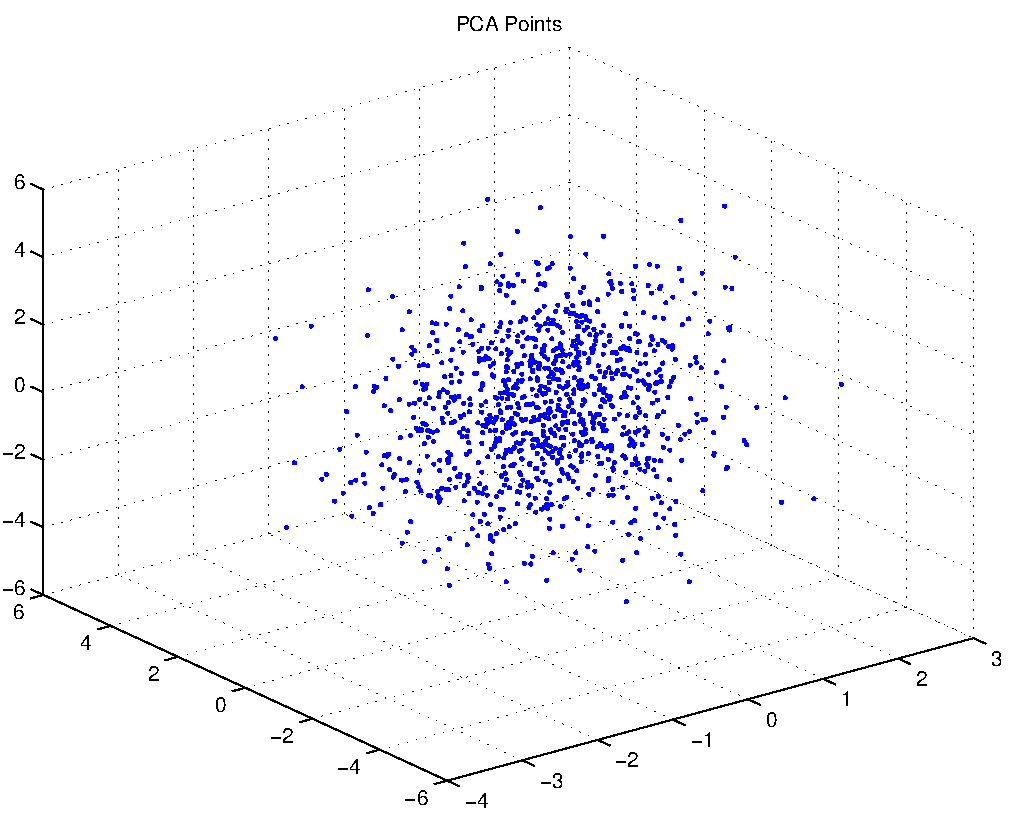
\includegraphics[width=10.0cm,height=10.0cm]{PCAPoints.pdf}

The eigenvectors:
+0.130, +0.182, +0.975
+0.155, +0.967, -0.202
-0.979, +0.177, +0.098

All of the eigenvalues of the covariance matrix:
(+0.958,+0.000), (+2.025,+0.000), (+3.017,+0.000)

QueryPerformanceCounter  =  +1.258
\subsubsection{Multi Variate Random Number Generator }
Sample from $N(\mu,\Sigma)$
mean= -0.002, variance=+1.004, skewness=+0.006, kurtosis=+3.003
mean= -0.001, variance=+1.017, skewness=-0.005, kurtosis=+2.988
mean= -0.002, variance=+1.006, skewness=-0.016, kurtosis=+3.014
Covariance Matrix 
+1.004, +0.009, +0.003
+0.009, +1.017, -0.003
+0.003, -0.003, +1.006

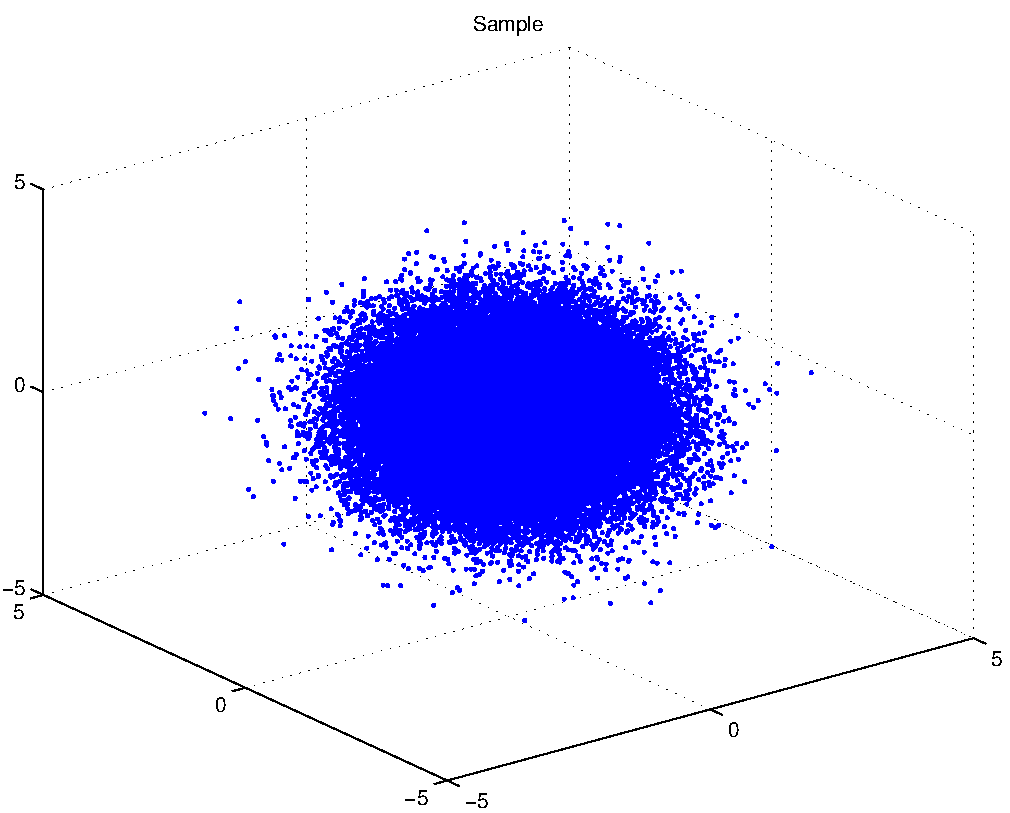
\includegraphics[width=10.0cm,height=10.0cm]{R_3_Normal.pdf}

Generate a sample from a unifom mixture of three Gaussians in $R^3$
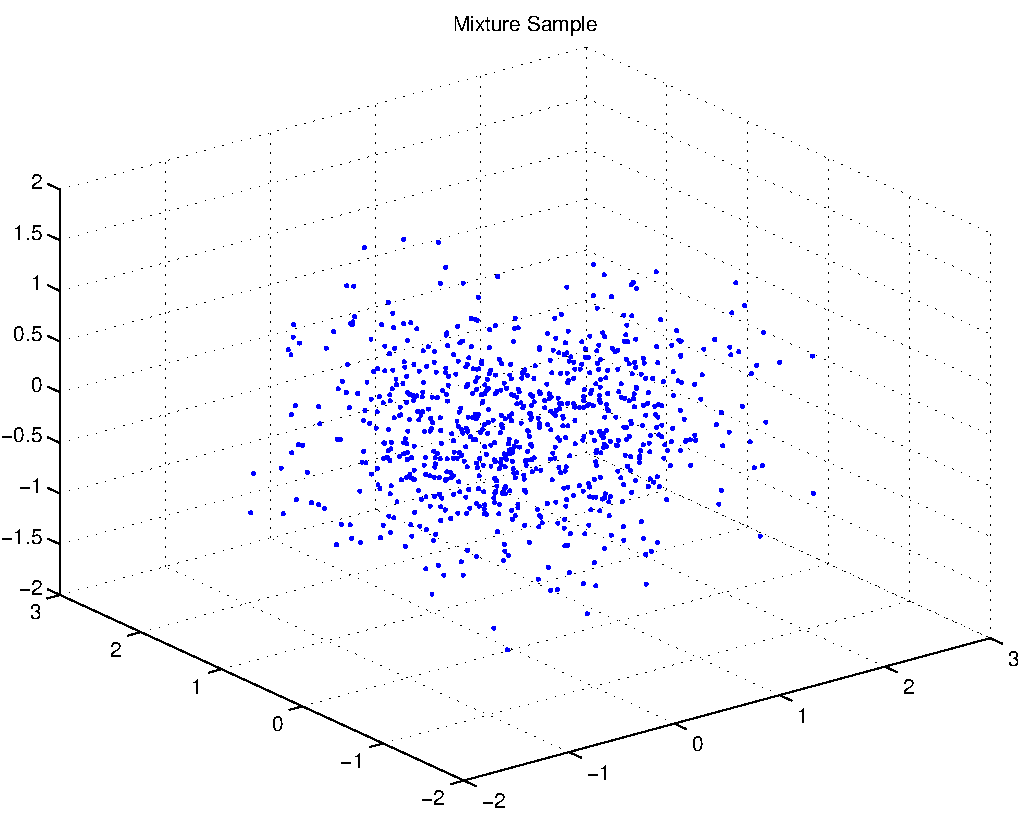
\includegraphics[width=10.0cm,height=10.0cm]{R_3_Normal_Mixture.pdf}

QueryPerformanceCounter  =  +17.759
\subsubsection{Matrix Multiply}
Comparing naive matrix multiply verus Intel MKL dgemm for matrix of size +2048.
This is for type double (hence the d in dgemm).
Naive type double matrix multiply tic toc  =  +0.429
dgemm plus row to column major transpose operation tic toc  =  +0.292
Comparing naive matrix multiply verus Intel MKL sgemm for matrix of size +2048.
This is for type float (hence the s in dgemm).
Naive type float matrix multiply tic toc  =  +0.224
sgemm plus row to column major transpose operation tic toc  =  +0.221
QueryPerformanceCounter  =  +1.306
\subsubsection{Descriptive Statistics}
Mean N(0,1): +0.003
Variance N(0,1): +1.006
Mean N(0,1) [recurrence relation method] :+0.003
Variance [recurrence relation method] :+1.006
Skewness : +0.007
Kurtosis : +2.997
QueryPerformanceCounter  =  +0.019
\subsubsection{Time Series }
+0.093
+0.726
+0.011
+2.178
QueryPerformanceCounter  =  +0.028
QueryPerformanceCounter  =  +5.822
\subsubsection{Iterated Exponential Filtering }
$\mu_1 =+0.093$
$\mu_2 =+0.726$
$\mu_3 =+0.011$
$\mu_4 =+2.178$
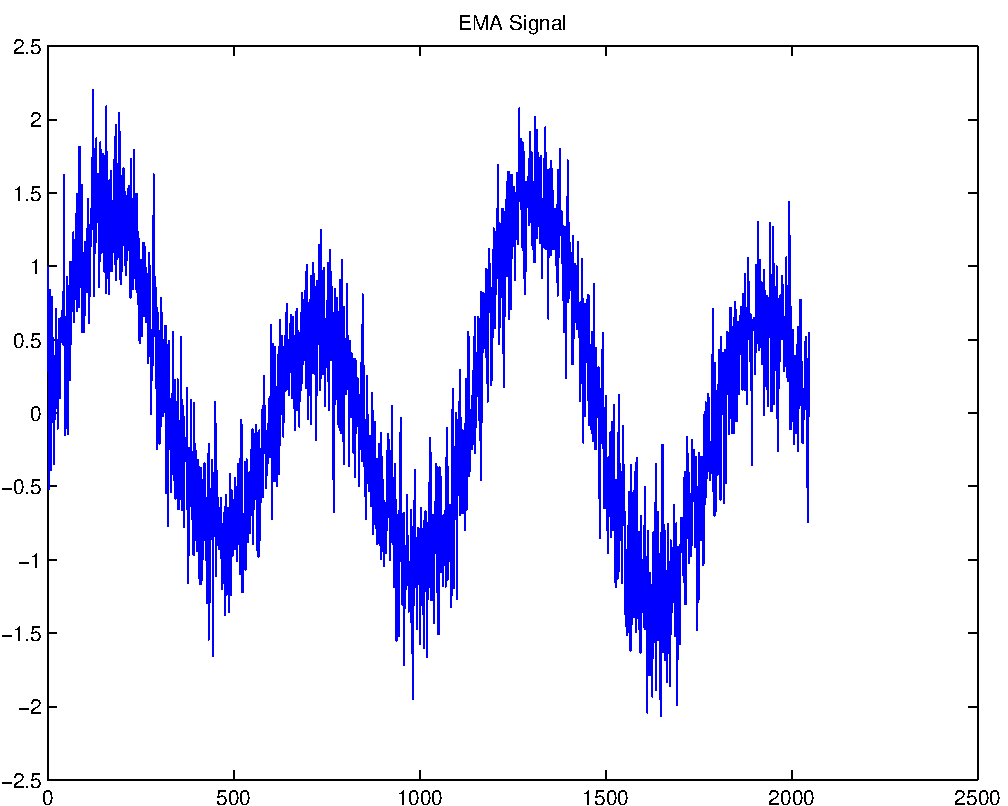
\includegraphics[width=10.0cm,height=10.0cm]{EMA_signal.pdf}

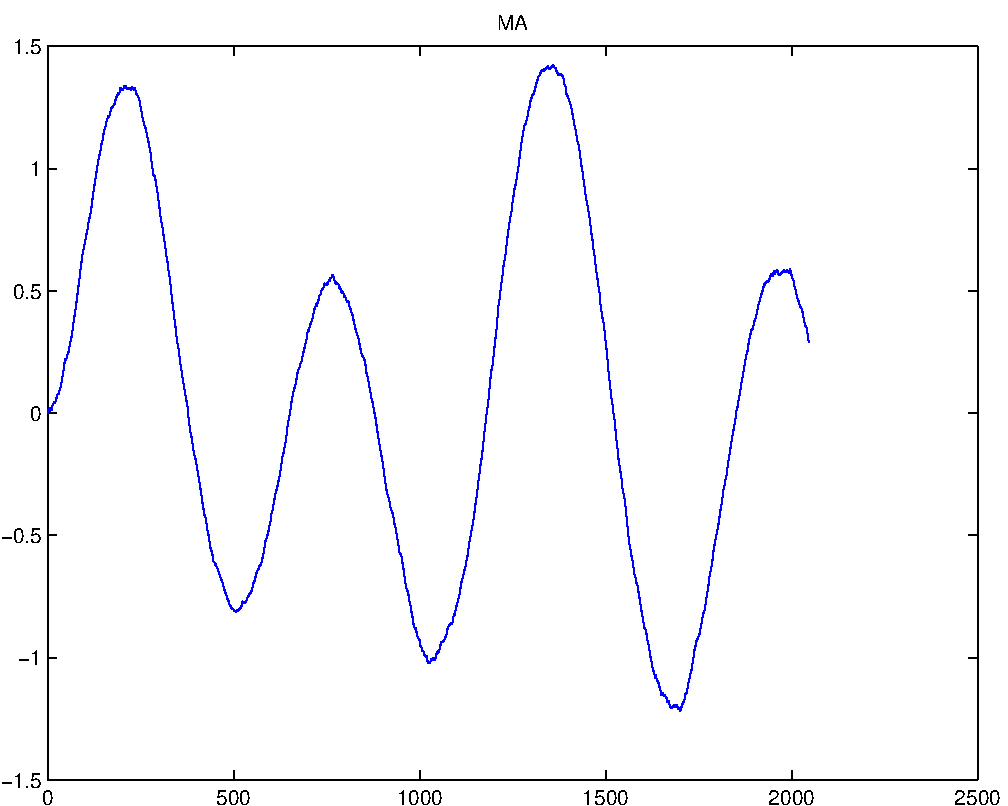
\includegraphics[width=10.0cm,height=10.0cm]{MA.pdf}

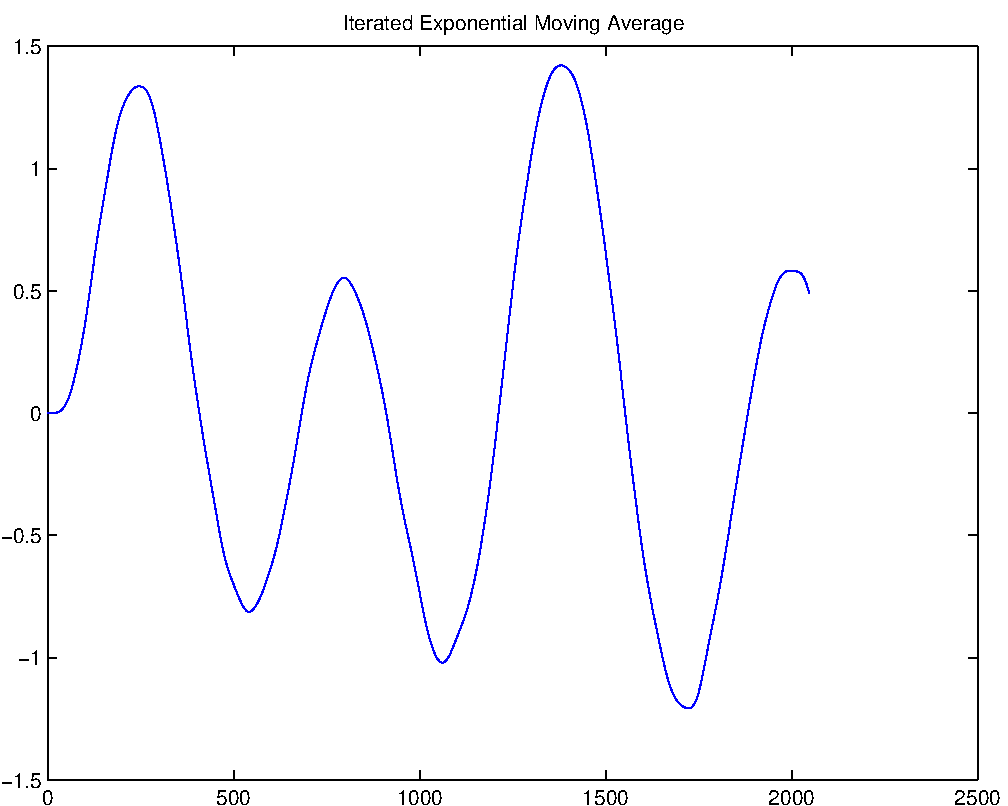
\includegraphics[width=10.0cm,height=10.0cm]{IEMA.pdf}

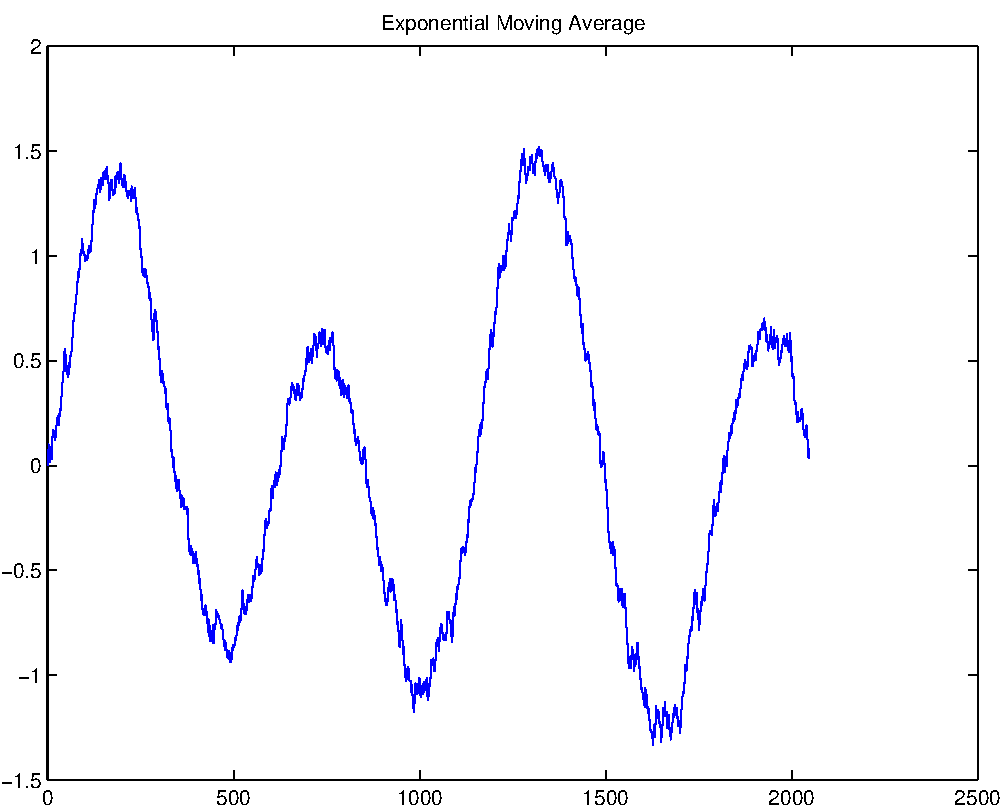
\includegraphics[width=10.0cm,height=10.0cm]{EMA.pdf}

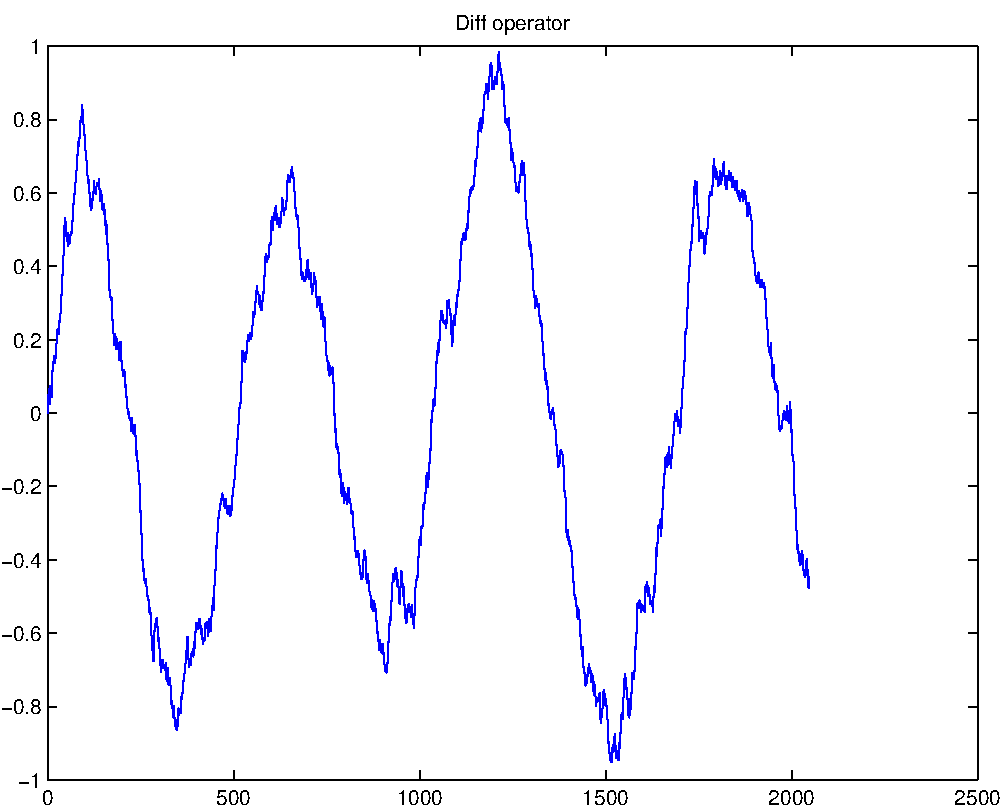
\includegraphics[width=10.0cm,height=10.0cm]{DIFF.pdf}

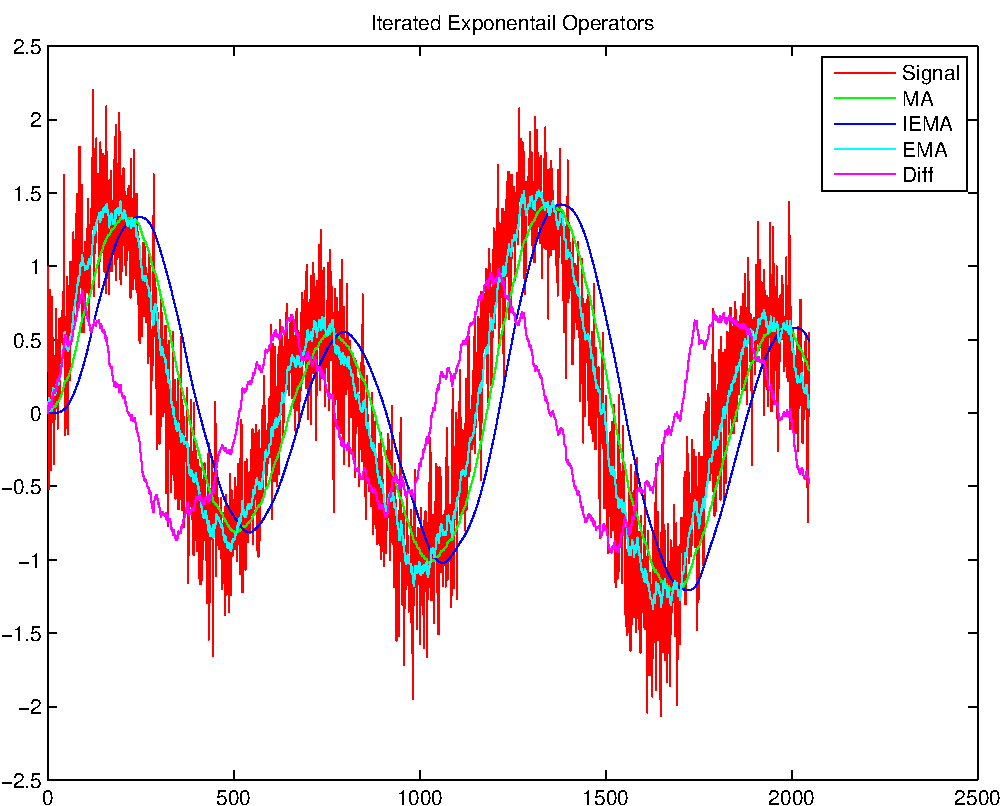
\includegraphics[width=10.0cm,height=10.0cm]{IteratedExponentailOperators.pdf}

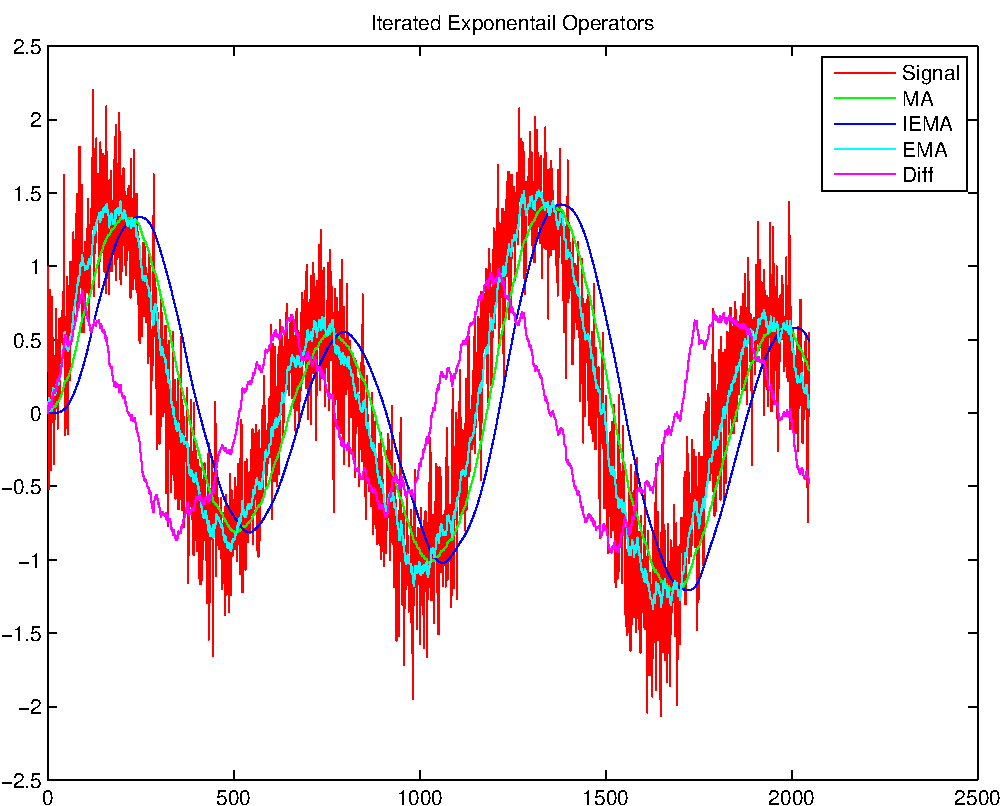
\includegraphics[width=10.0cm,height=10.0cm]{IteratedExponentailOperators.pdf}

QueryPerformanceCounter  =  +7.804
\subsubsection{Testing binary writer}
Binary writer Speedup 1GB Double Matrix +50.503

Binary reader Speedup 1GB Double Matrix +199.947

Binary writer Speedup 1GB Double vector +10.005

Binary reader Speedup 1GB Double Matrix +176.176

QueryPerformanceCounter  =  +0.879
\subsubsection{Testing Gaussian Mixture Point Cloud and Latex Plotting Capabilities.}
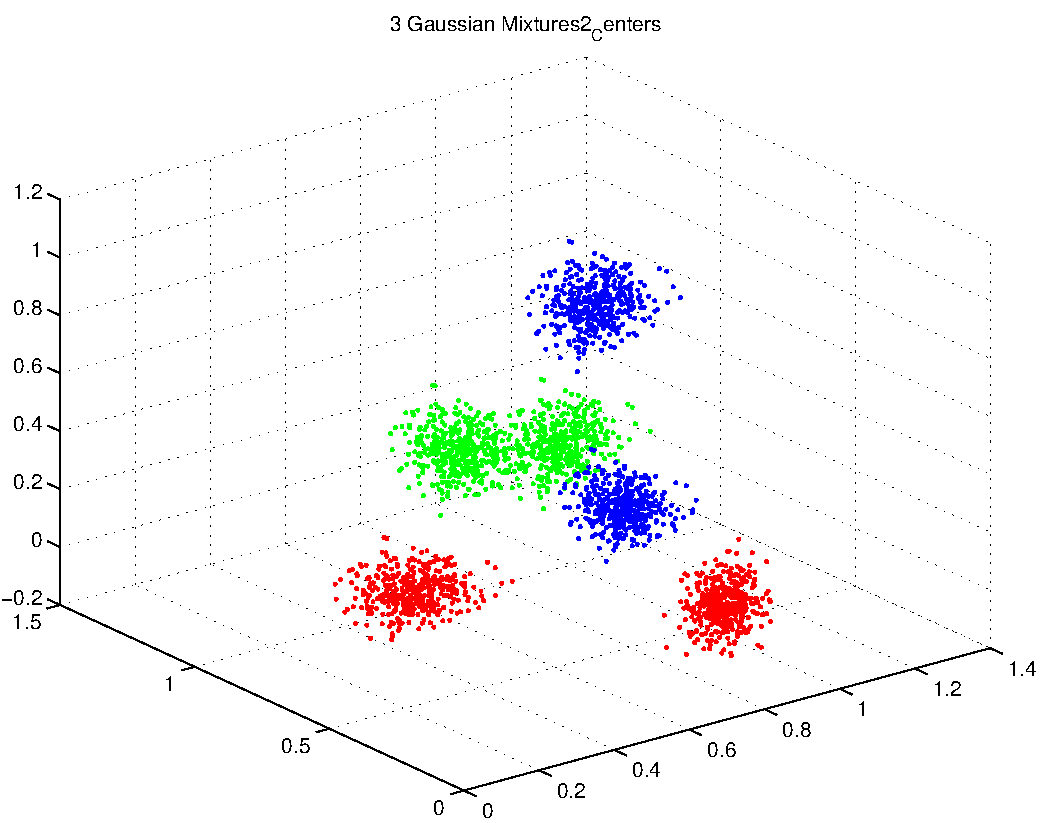
\includegraphics[width=10.0cm,height=10.0cm]{GaussianMixture_Dim_3_Centers2.pdf}

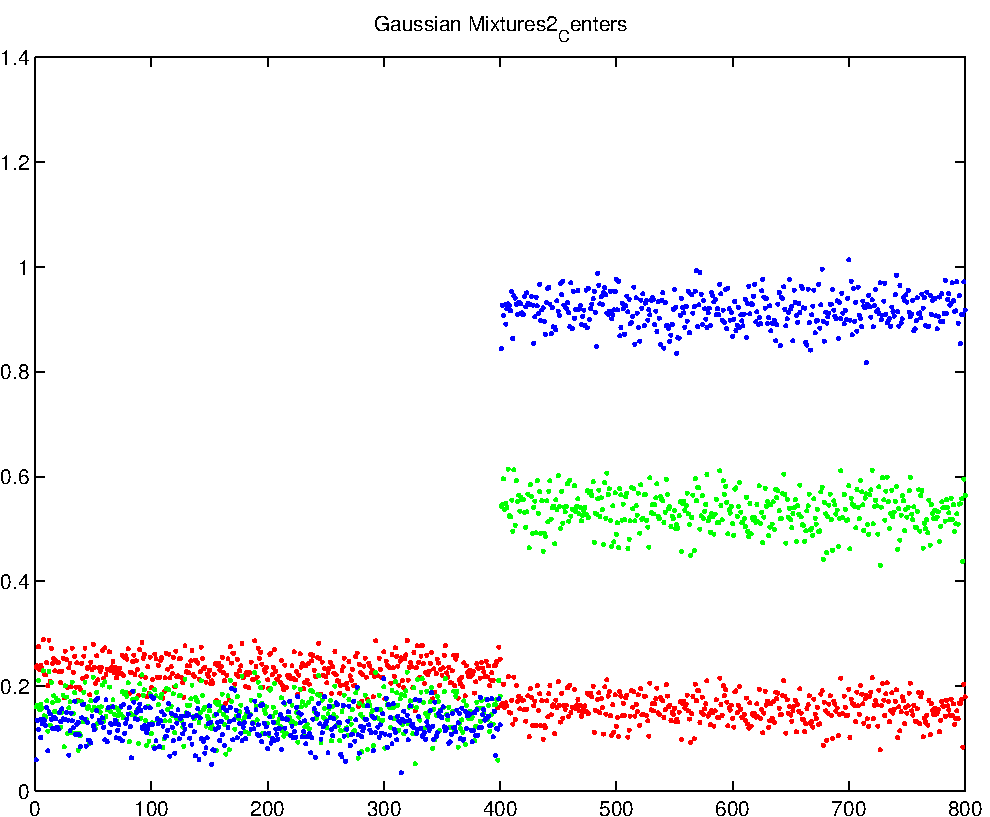
\includegraphics[width=10.0cm,height=10.0cm]{GaussianMixture_Dim_1_Centers2.pdf}

QueryPerformanceCounter  =  +2.690
\subsubsection{Intel VSL Function Check}
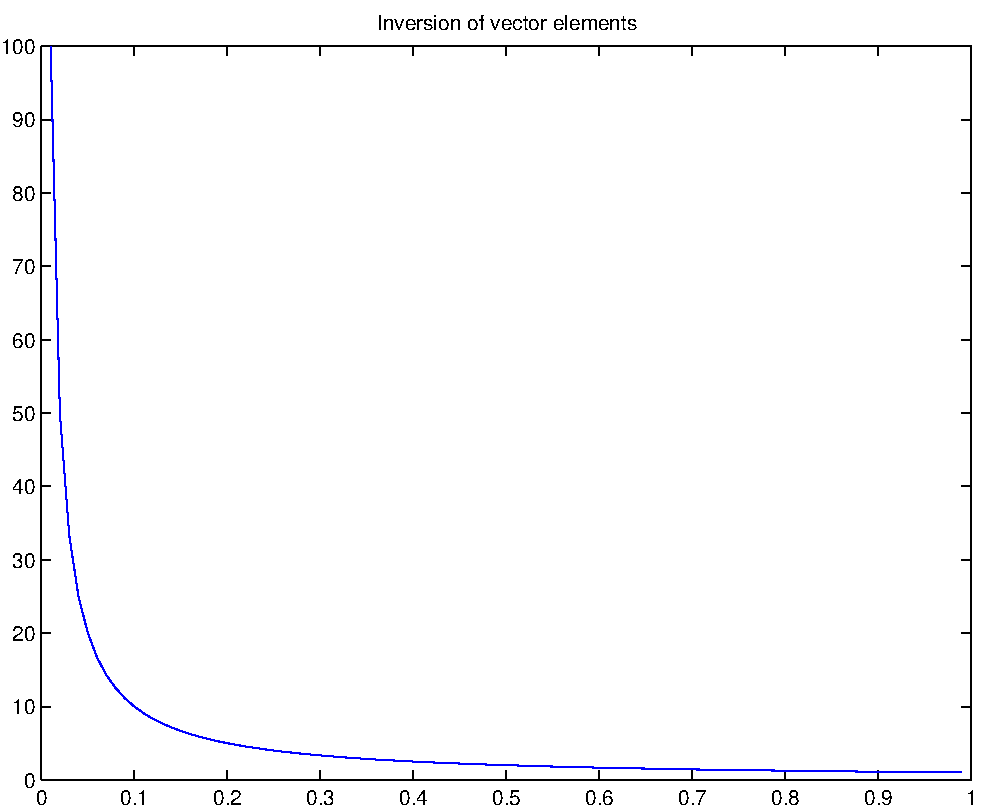
\includegraphics[width=10.0cm,height=10.0cm]{klVSLInv.pdf}

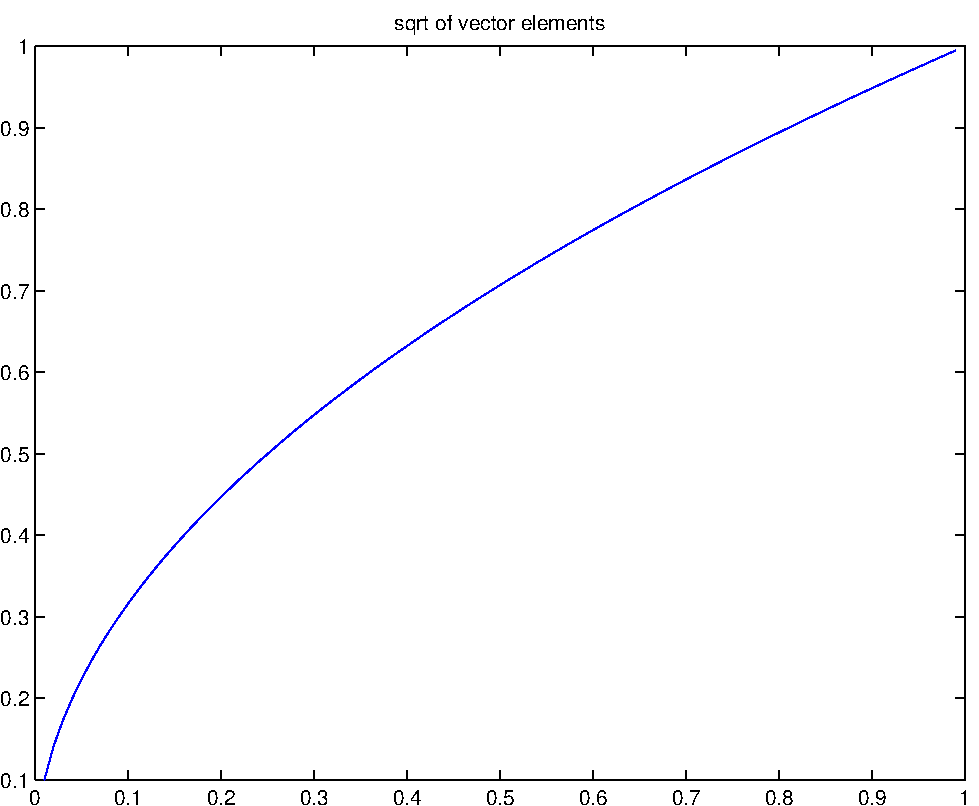
\includegraphics[width=10.0cm,height=10.0cm]{klVSLSqrt.pdf}

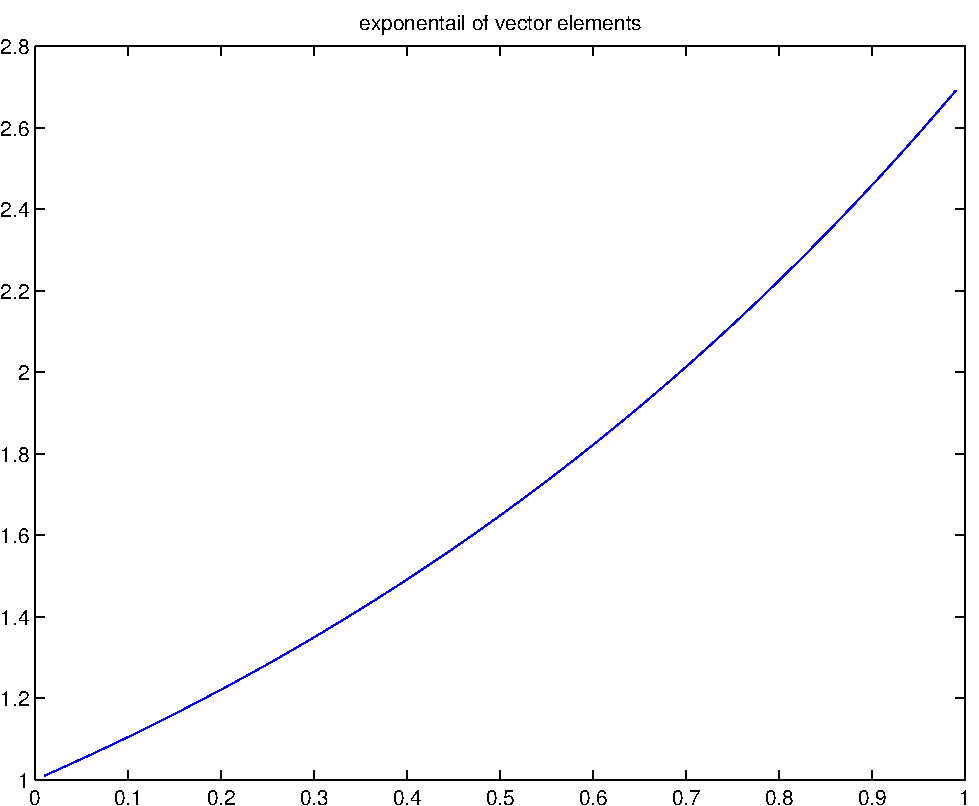
\includegraphics[width=10.0cm,height=10.0cm]{klVSLExp.pdf}

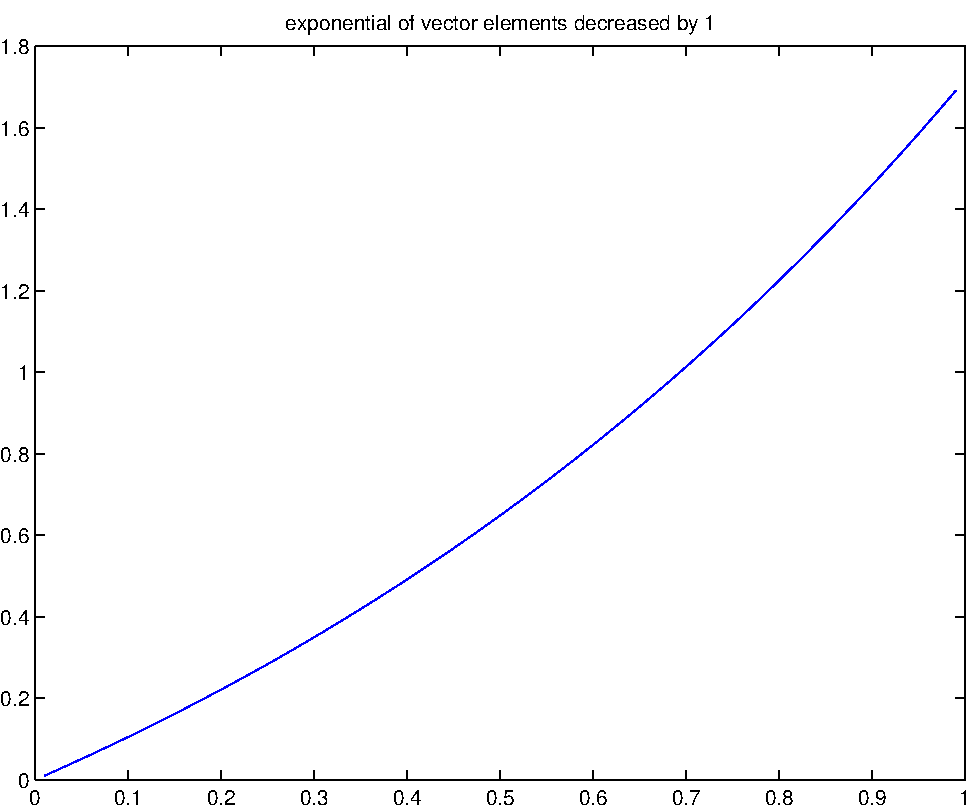
\includegraphics[width=10.0cm,height=10.0cm]{klVSLExpm1.pdf}

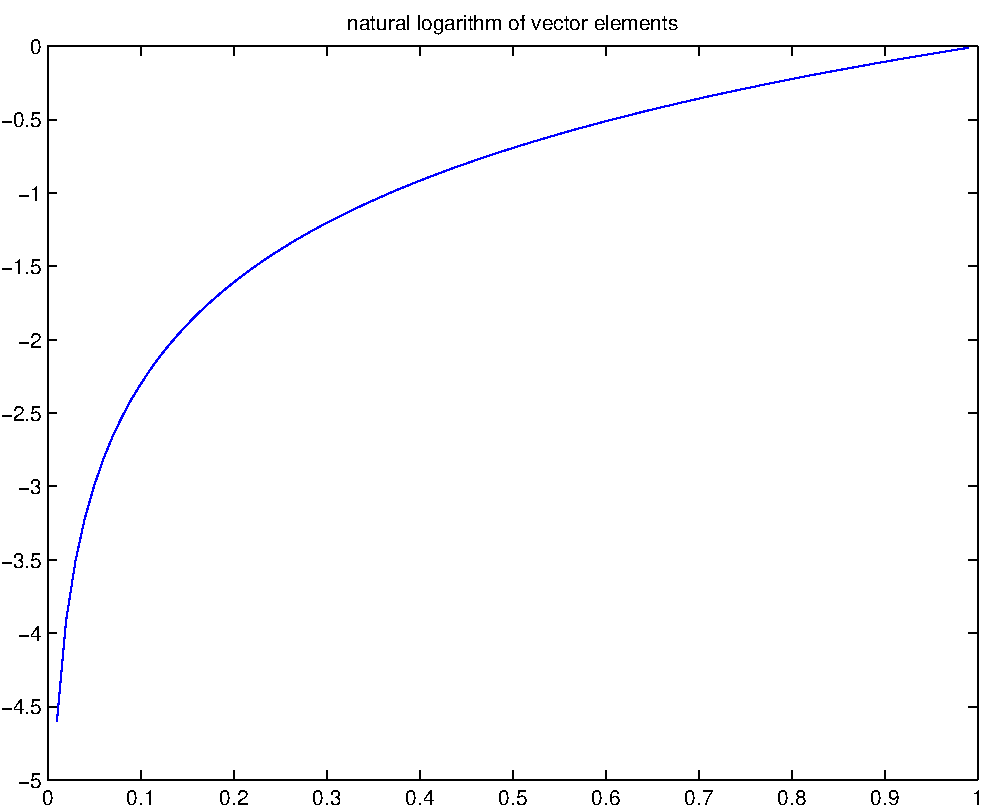
\includegraphics[width=10.0cm,height=10.0cm]{klVSLLn.pdf}

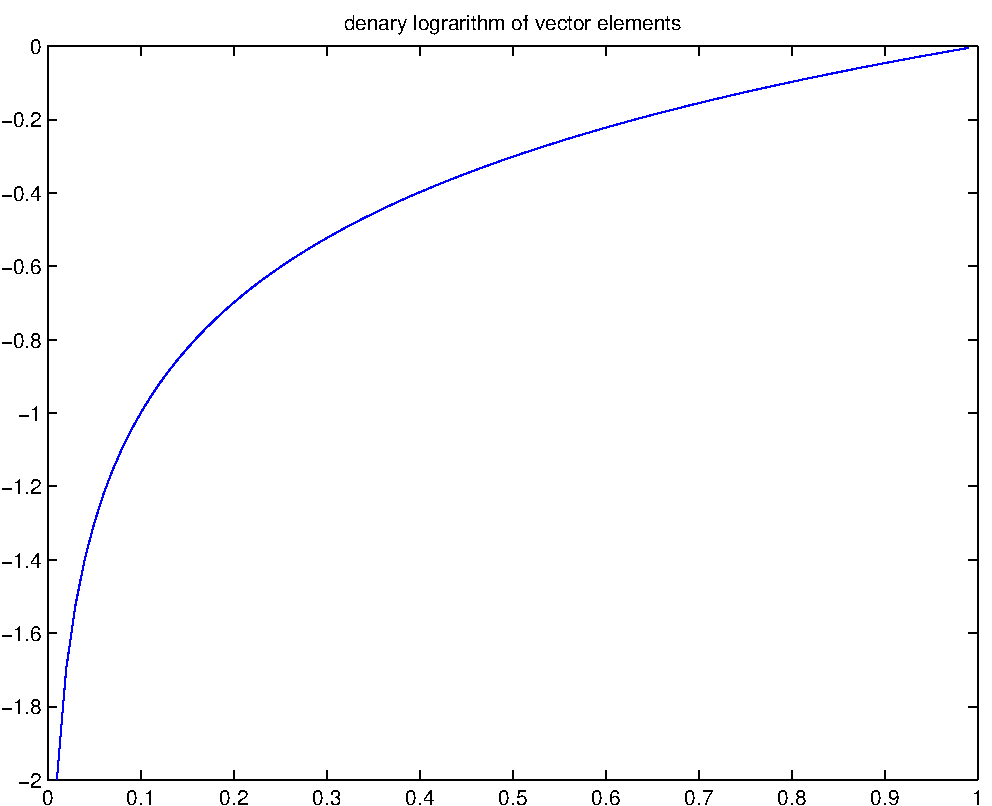
\includegraphics[width=10.0cm,height=10.0cm]{klVSLLog10.pdf}

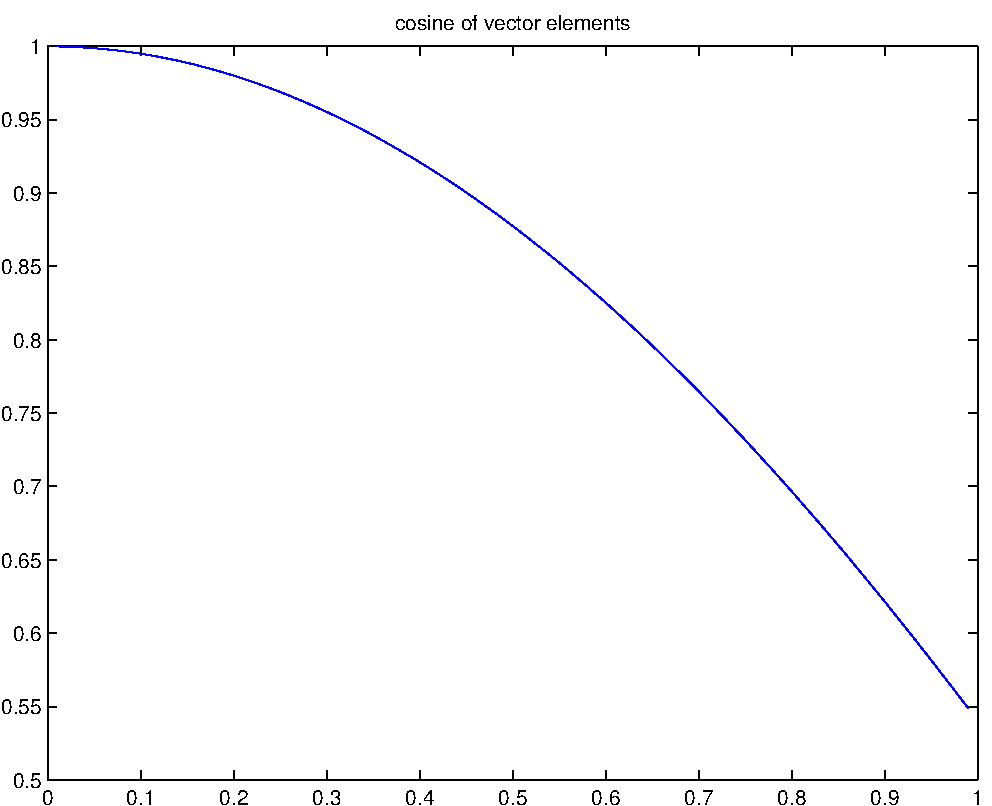
\includegraphics[width=10.0cm,height=10.0cm]{klVSLCos.pdf}

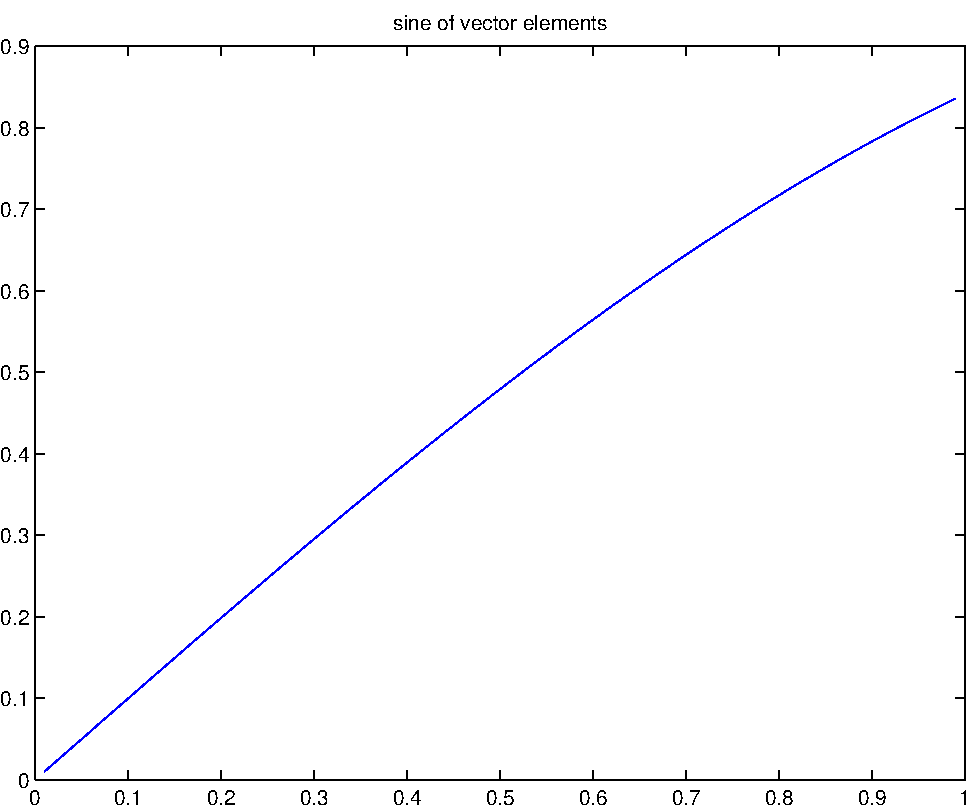
\includegraphics[width=10.0cm,height=10.0cm]{klVSLSin.pdf}

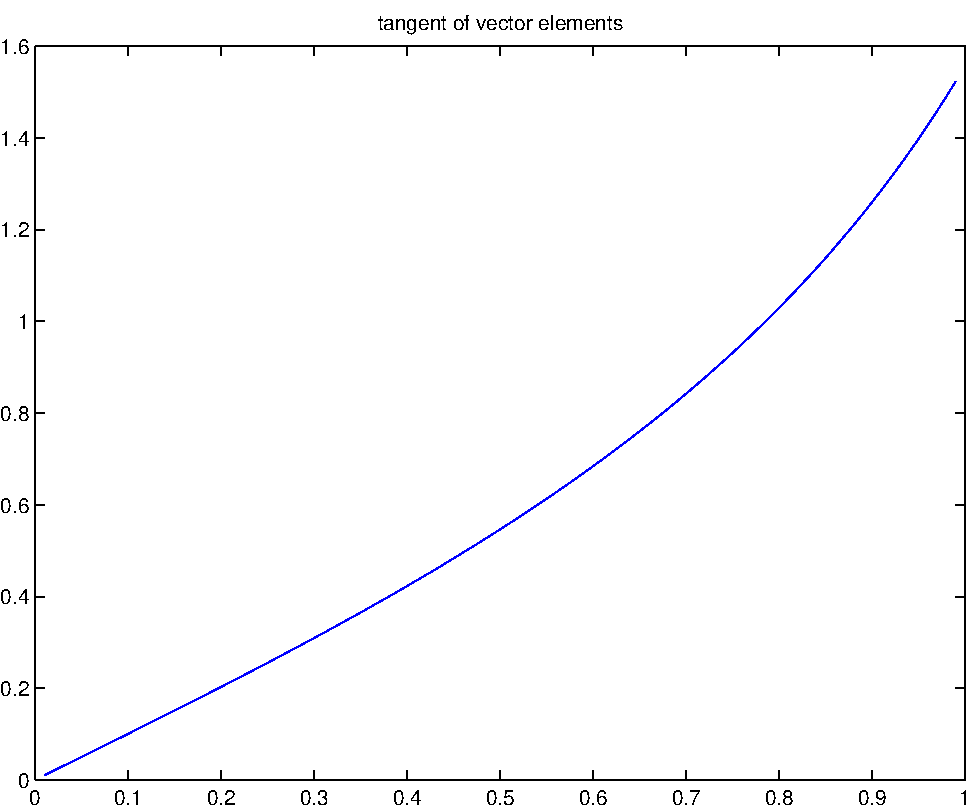
\includegraphics[width=10.0cm,height=10.0cm]{klVSLTan.pdf}

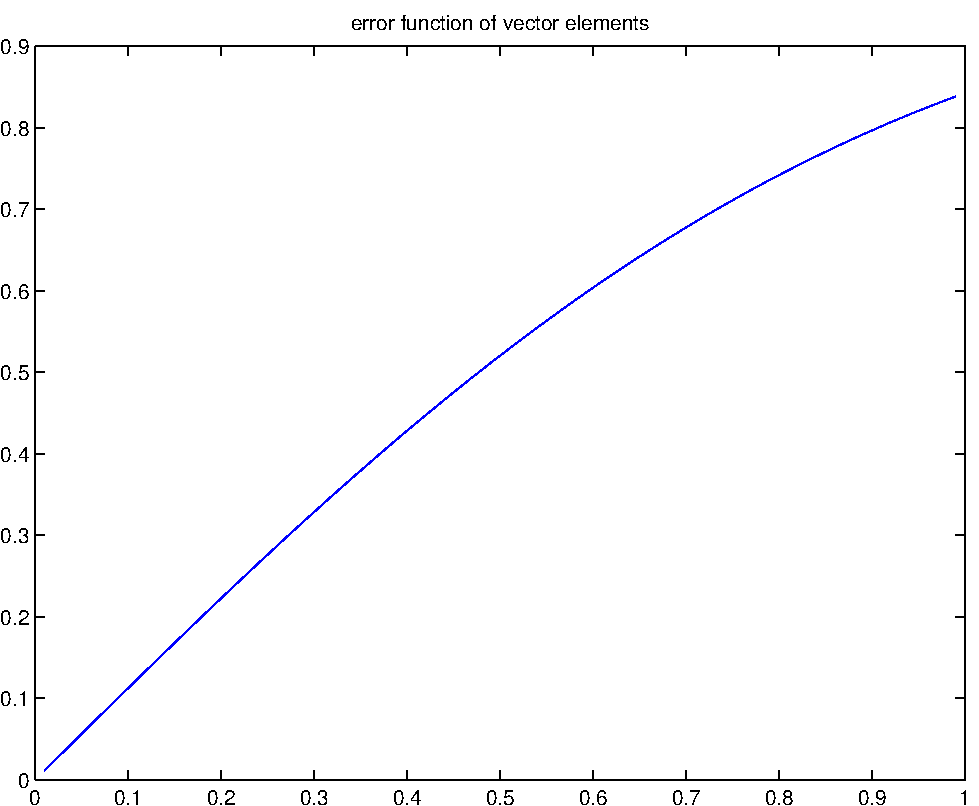
\includegraphics[width=10.0cm,height=10.0cm]{klVSLErf.pdf}

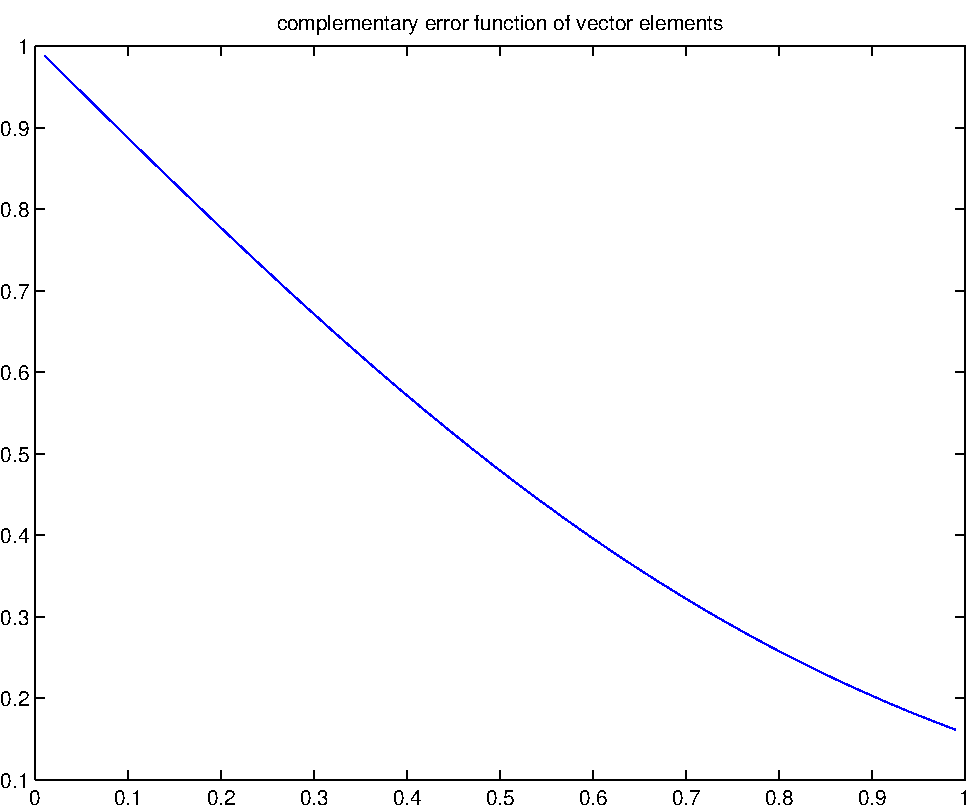
\includegraphics[width=10.0cm,height=10.0cm]{klVSLErfc.pdf}

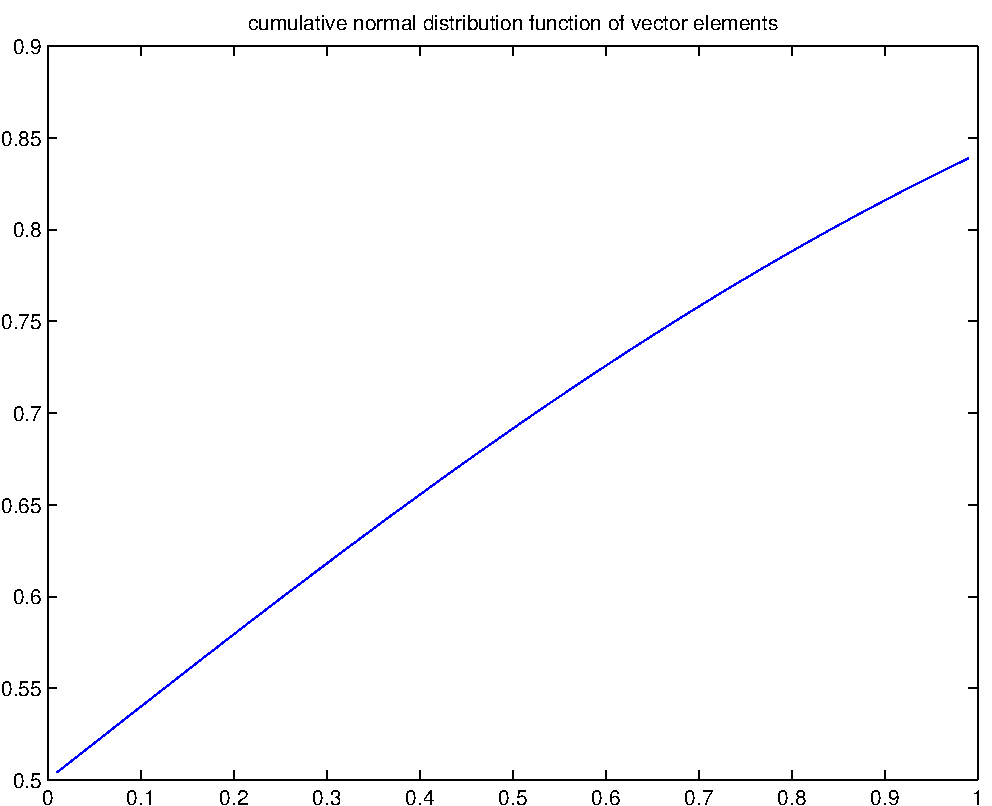
\includegraphics[width=10.0cm,height=10.0cm]{klVSLCdfNorm.pdf}

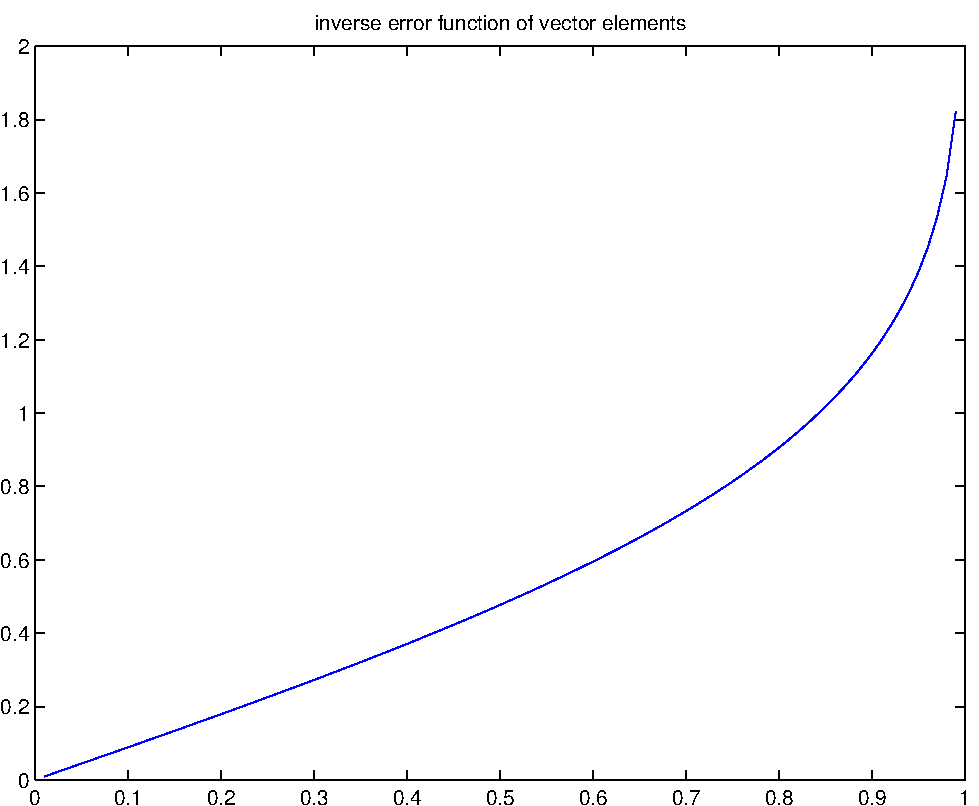
\includegraphics[width=10.0cm,height=10.0cm]{klVSLErfInv.pdf}

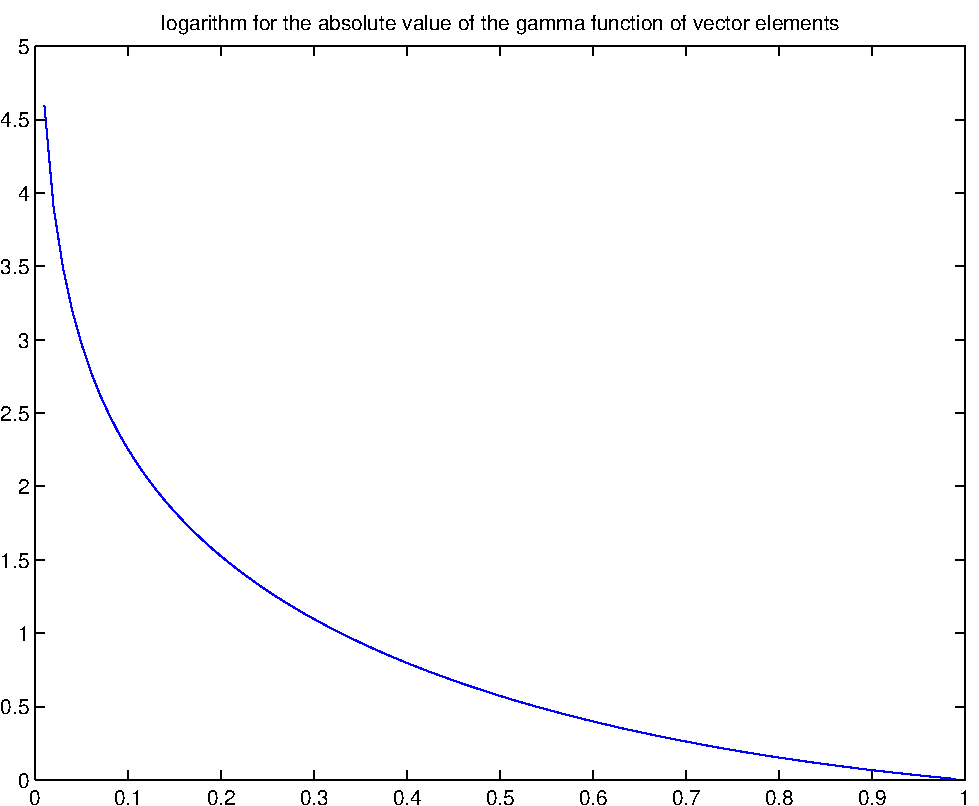
\includegraphics[width=10.0cm,height=10.0cm]{klVSLLGamma.pdf}

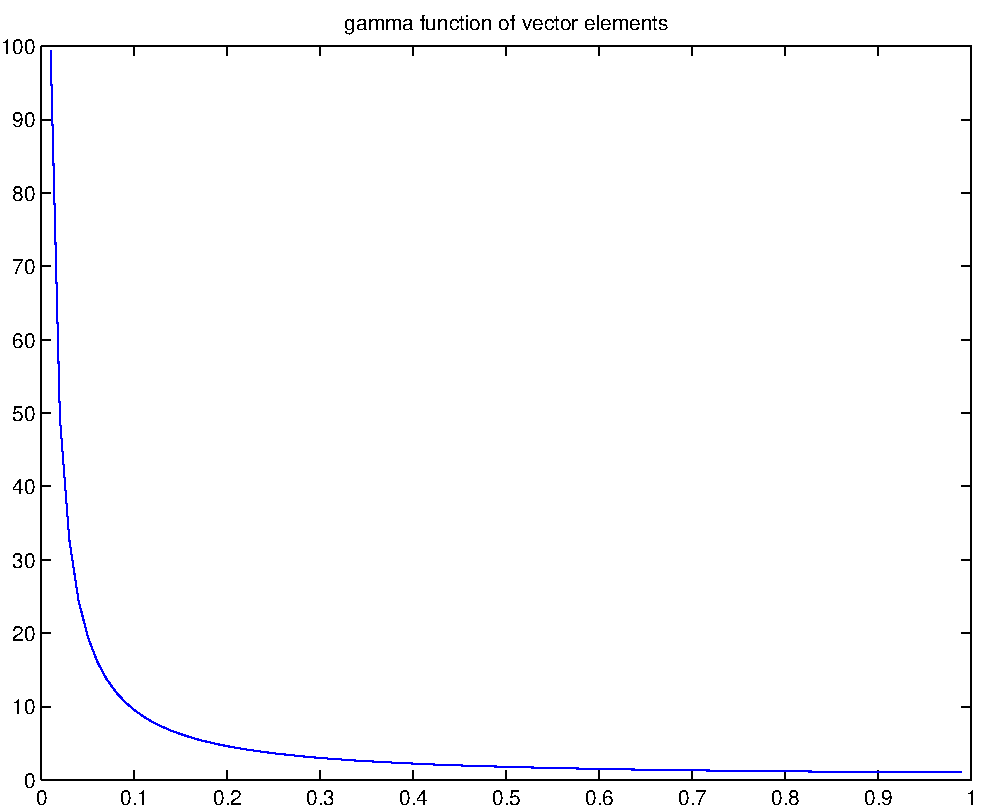
\includegraphics[width=10.0cm,height=10.0cm]{klVSLTGamma.pdf}

QueryPerformanceCounter  =  +15.366
\subsubsection{Gram Matrix Consistency Check}
Sample Size = 4096
Feature dim = 3

$$Sigma$ = \left(
\begin{array}{
ccc}
+1.140 & +1.535 & +0.581 \\
+1.535 & +9.988 & +1.605 \\
+0.581 & +1.605 & +0.428 \\
\end{array}
\right)$ \newline 

$Sample Covariance = \left(
\begin{array}{
ccc}
+1.155 & +1.591 & +0.602 \\
+1.591 & +10.314 & +1.675 \\
+0.602 & +1.675 & +0.448 \\
\end{array}
\right)$ \newline 

$Sample Mean = \left(
\begin{array}{
ccc}
+1.02427 & +1.00175 & +1.01236 \\
\end{array}
\right)$ \newline 

$Sample Covariance-$Omega$ = \left(
\begin{array}{
ccc}
+0.015 & +0.056 & +0.020 \\
+0.056 & +0.325 & +0.069 \\
+0.020 & +0.069 & +0.020 \\
\end{array}
\right)$ \newline 

$Sample Covariance Eigs = \left(
\begin{array}{
ccc}
(+10.87644,+0.00000) & (+1.00005,+0.00000) & (+0.03986,+0.00000) \\
\end{array}
\right)$ \newline 

$Centered Mean = \left(
\begin{array}{
ccc}
-0.00000 & -0.00000 & +0.00000 \\
\end{array}
\right)$ \newline 

$Centered Covariance = \left(
\begin{array}{
ccc}
+1.155 & +1.591 & +0.602 \\
+1.591 & +10.314 & +1.675 \\
+0.602 & +1.675 & +0.448 \\
\end{array}
\right)$ \newline 

$Gram Matrix Gf Not scaled by sample size = \left(
\begin{array}{
ccc}
+4731.031 & +6514.214 & +2463.810 \\
+6514.214 & +42244.378 & +6857.863 \\
+2463.810 & +6857.863 & +1833.945 \\
\end{array}
\right)$ \newline 

$Gram Matrix Gf  scaled by sample size = \left(
\begin{array}{
ccc}
+1.155 & +1.590 & +0.602 \\
+1.590 & +10.314 & +1.674 \\
+0.602 & +1.674 & +0.448 \\
\end{array}
\right)$ \newline 

$SampleCovariance - Scaled Gf = \left(
\begin{array}{
ccc}
+0.000 & +0.000 & +0.000 \\
+0.000 & +0.003 & +0.000 \\
+0.000 & +0.000 & +0.000 \\
\end{array}
\right)$ \newline 

$EigenDecomp of SampleCovariance = \left(
\begin{array}{
ccc}
-0.169 & -0.972 & -0.166 \\
+0.916 & -0.217 & +0.339 \\
-0.365 & -0.094 & +0.926 \\
\end{array}
\right)$ \newline 

$EigenDecomp of Gram Matrix = \left(
\begin{array}{
ccc}
-0.117 & -0.975 & -0.189 \\
-0.317 & +0.217 & -0.923 \\
+0.941 & -0.049 & -0.334 \\
\end{array}
\right)$ \newline 

QueryPerformanceCounter  =  +1.387
\subsubsection{Eigen Solver Checks}
\subsubsection{Haar Distributed Random Orthogonal Matrix $A \in O(n)$}
 Testing Operator Norm
Number of Dimensions: +8

$A = \left(
\begin{array}{
cccccccc}
+0.136 & -0.285 & -0.795 & +0.141 & -0.191 & -0.117 & -0.201 & +0.396 \\
+0.684 & +0.249 & -0.160 & +0.365 & +0.290 & +0.419 & +0.039 & -0.224 \\
+0.063 & +0.306 & +0.151 & +0.460 & -0.787 & -0.084 & +0.201 & +0.036 \\
+0.063 & +0.034 & -0.160 & +0.197 & +0.310 & -0.713 & +0.544 & -0.173 \\
+0.430 & -0.598 & +0.187 & -0.103 & -0.276 & -0.233 & -0.223 & -0.482 \\
+0.514 & +0.297 & +0.036 & -0.680 & -0.157 & -0.145 & +0.182 & +0.325 \\
+0.155 & -0.529 & +0.366 & +0.211 & +0.110 & +0.194 & +0.413 & +0.545 \\
-0.178 & -0.190 & -0.351 & -0.282 & -0.228 & +0.427 & +0.608 & -0.356 \\
\end{array}
\right)$ \newline 

$Det(A) :   A \in O(n)$ = (+1.000,+0.000)

$L = \left(
\begin{array}{
cccccccc}
+1.000 & +0.000 & +0.000 & +0.000 & +0.000 & +0.000 & +0.000 & +0.000 \\
+0.629 & +1.000 & +0.000 & +0.000 & +0.000 & +0.000 & +0.000 & +0.000 \\
+0.199 & +0.444 & +1.000 & +0.000 & +0.000 & +0.000 & +0.000 & +0.000 \\
+0.751 & -0.145 & -0.222 & +1.000 & +0.000 & +0.000 & +0.000 & +0.000 \\
+0.093 & -0.375 & -0.307 & -0.386 & +1.000 & +0.000 & +0.000 & +0.000 \\
+0.092 & -0.015 & +0.159 & -0.131 & -0.192 & +1.000 & +0.000 & +0.000 \\
-0.260 & +0.166 & +0.493 & +0.249 & -0.050 & -0.769 & +1.000 & +0.000 \\
+0.227 & +0.777 & -0.201 & -0.449 & -0.160 & -0.185 & +0.653 & +1.000 \\
\end{array}
\right)$ \newline 

$U = \left(
\begin{array}{
cccccccc}
+0.684 & +0.249 & -0.160 & +0.365 & +0.290 & +0.419 & +0.039 & -0.224 \\
+0.000 & -0.754 & +0.288 & -0.332 & -0.458 & -0.496 & -0.247 & -0.341 \\
+0.000 & +0.000 & -0.891 & +0.215 & -0.046 & +0.021 & -0.099 & +0.592 \\
+0.000 & +0.000 & +0.000 & -0.954 & -0.451 & -0.527 & +0.096 & +0.575 \\
+0.000 & +0.000 & +0.000 & +0.000 & -1.173 & -0.506 & +0.111 & +0.333 \\
+0.000 & +0.000 & +0.000 & +0.000 & +0.000 & -0.928 & +0.586 & -0.113 \\
+0.000 & +0.000 & +0.000 & +0.000 & +0.000 & +0.000 & +1.140 & -0.863 \\
+0.000 & +0.000 & +0.000 & +0.000 & +0.000 & +0.000 & +0.000 & +1.834 \\
\end{array}
\right)$ \newline 

$L * U  = \left(
\begin{array}{
cccccccc}
+0.684 & +0.249 & -0.160 & +0.365 & +0.290 & +0.419 & +0.039 & -0.224 \\
+0.430 & -0.598 & +0.187 & -0.103 & -0.276 & -0.233 & -0.223 & -0.482 \\
+0.136 & -0.285 & -0.795 & +0.141 & -0.191 & -0.117 & -0.201 & +0.396 \\
+0.514 & +0.297 & +0.036 & -0.680 & -0.157 & -0.145 & +0.182 & +0.325 \\
+0.063 & +0.306 & +0.151 & +0.460 & -0.787 & -0.084 & +0.201 & +0.036 \\
+0.063 & +0.034 & -0.160 & +0.197 & +0.310 & -0.713 & +0.544 & -0.173 \\
-0.178 & -0.190 & -0.351 & -0.282 & -0.228 & +0.427 & +0.608 & -0.356 \\
+0.155 & -0.529 & +0.366 & +0.211 & +0.110 & +0.194 & +0.413 & +0.545 \\
\end{array}
\right)$ \newline 

$Det(L) :    = (+1.000,+0.000)     Det(U) :    = (-1.000,+0.000)     Det(LU) :    = (-1.000,+0.000)$

$||A||_{L_1}$  = +2.537

$||A||_{L_{\infty}}$ = +2.618

$||A^{-1}||_{L_1}$  = +2.618

$||A^{-1}||_{L_{\infty}}$ = +2.537

$||A||_{L_{\infty}} * ||A^{-1}||_{L_{\infty}} = +6.644$

$||A||_{L_1} * ||A^{-1}||_{L_1} = +6.644$

Frobenious Norm  $||A||_{\textit{F}}$ via $\sum\limits_{i,j =0}^{n} \|A_{i,j}|$   of  $A \in O(n)$  +2.828

$L_1$ condition number of Haar Distributed Random Orthogonal Matrix $A \in O(n)$ +5.742

$A = \left(
\begin{array}{
cccccccc}
+0.136 & -0.285 & -0.795 & +0.141 & -0.191 & -0.117 & -0.201 & +0.396 \\
+0.684 & +0.249 & -0.160 & +0.365 & +0.290 & +0.419 & +0.039 & -0.224 \\
+0.063 & +0.306 & +0.151 & +0.460 & -0.787 & -0.084 & +0.201 & +0.036 \\
+0.063 & +0.034 & -0.160 & +0.197 & +0.310 & -0.713 & +0.544 & -0.173 \\
+0.430 & -0.598 & +0.187 & -0.103 & -0.276 & -0.233 & -0.223 & -0.482 \\
+0.514 & +0.297 & +0.036 & -0.680 & -0.157 & -0.145 & +0.182 & +0.325 \\
+0.155 & -0.529 & +0.366 & +0.211 & +0.110 & +0.194 & +0.413 & +0.545 \\
-0.178 & -0.190 & -0.351 & -0.282 & -0.228 & +0.427 & +0.608 & -0.356 \\
\end{array}
\right)$ \newline 

$L_{\infty}$ condition number of Haar Distributed Random Orthogonal Matrix $A \in O(n)$ +6.515

Eigenvalues of $A \in O(n)$

(-0.349,+0.937), (-0.349,-0.937), (+0.536,+0.844), (+0.536,-0.844), (-0.999,+0.038), (-0.999,-0.038), (+0.997,+0.077), (+0.997,-0.077)

 $|\lambda | : \lambda \in \sigma(A) , A \in O(n)$

+1.000, +1.000, +1.000, +1.000, +1.000, +1.000, +1.000, +1.000


Calculating $A^{\dag} A,$  we expect $A^{\dag} A \approx I$

$A^{\dag} A = \left(
\begin{array}{
cccccccc}
+1.000 & +0.000 & +0.000 & +0.000 & +0.000 & +0.000 & +0.000 & -0.000 \\
+0.000 & +1.000 & +0.000 & +0.000 & -0.000 & -0.000 & -0.000 & -0.000 \\
+0.000 & +0.000 & +1.000 & +0.000 & -0.000 & +0.000 & +0.000 & +0.000 \\
+0.000 & +0.000 & +0.000 & +1.000 & -0.000 & -0.000 & +0.000 & +0.000 \\
+0.000 & -0.000 & -0.000 & -0.000 & +1.000 & +0.000 & -0.000 & +0.000 \\
+0.000 & -0.000 & +0.000 & -0.000 & +0.000 & +1.000 & +0.000 & +0.000 \\
+0.000 & -0.000 & +0.000 & +0.000 & -0.000 & +0.000 & +1.000 & +0.000 \\
-0.000 & -0.000 & +0.000 & +0.000 & +0.000 & +0.000 & +0.000 & +1.000 \\
\end{array}
\right)$ \newline 

Calculating $A^{-1} ,  A \in O(n)$.

$A^{-1} = \left(
\begin{array}{
cccccccc}
+0.136 & +0.684 & +0.063 & +0.063 & +0.430 & +0.514 & +0.155 & -0.178 \\
-0.285 & +0.249 & +0.306 & +0.034 & -0.598 & +0.297 & -0.529 & -0.190 \\
-0.795 & -0.160 & +0.151 & -0.160 & +0.187 & +0.036 & +0.366 & -0.351 \\
+0.141 & +0.365 & +0.460 & +0.197 & -0.103 & -0.680 & +0.211 & -0.282 \\
-0.191 & +0.290 & -0.787 & +0.310 & -0.276 & -0.157 & +0.110 & -0.228 \\
-0.117 & +0.419 & -0.084 & -0.713 & -0.233 & -0.145 & +0.194 & +0.427 \\
-0.201 & +0.039 & +0.201 & +0.544 & -0.223 & +0.182 & +0.413 & +0.608 \\
+0.396 & -0.224 & +0.036 & -0.173 & -0.482 & +0.325 & +0.545 & -0.356 \\
\end{array}
\right)$ \newline 

Calculating $A^{-1} *A  ,  A \in O(n)$.   We expect $A^{-1} *A  \approx I$. 

$A^{-1} *A = \left(
\begin{array}{
cccccccc}
+1.000 & +0.000 & -0.000 & +0.000 & -0.000 & +0.000 & +0.000 & -0.000 \\
+0.000 & +1.000 & -0.000 & +0.000 & +0.000 & -0.000 & -0.000 & +0.000 \\
+0.000 & +0.000 & +1.000 & +0.000 & -0.000 & +0.000 & +0.000 & -0.000 \\
-0.000 & -0.000 & +0.000 & +1.000 & -0.000 & +0.000 & -0.000 & -0.000 \\
-0.000 & -0.000 & -0.000 & -0.000 & +1.000 & +0.000 & +0.000 & +0.000 \\
+0.000 & +0.000 & +0.000 & -0.000 & +0.000 & +1.000 & -0.000 & -0.000 \\
-0.000 & -0.000 & +0.000 & +0.000 & +0.000 & -0.000 & +1.000 & -0.000 \\
-0.000 & -0.000 & +0.000 & +0.000 & -0.000 & +0.000 & +0.000 & +1.000 \\
\end{array}
\right)$ \newline 

Calculating SVD of  $A \in O(n)$

$U = \left(
\begin{array}{
cccccccc}
-0.224 & +0.096 & -0.159 & -0.099 & -0.720 & -0.035 & -0.189 & -0.592 \\
-0.398 & -0.146 & +0.030 & -0.795 & +0.092 & +0.014 & -0.343 & +0.249 \\
-0.105 & +0.216 & +0.427 & +0.353 & -0.284 & -0.303 & -0.526 & +0.432 \\
-0.243 & +0.126 & +0.049 & +0.034 & -0.419 & +0.632 & +0.388 & +0.442 \\
-0.136 & +0.285 & +0.795 & -0.141 & +0.191 & +0.117 & +0.201 & -0.396 \\
-0.312 & -0.798 & +0.262 & +0.167 & -0.148 & -0.259 & +0.284 & -0.005 \\
-0.666 & +0.029 & -0.208 & +0.427 & +0.397 & +0.275 & -0.255 & -0.176 \\
-0.401 & +0.433 & -0.210 & -0.059 & +0.029 & -0.593 & +0.483 & +0.134 \\
\end{array}
\right)$ \newline 

$S = \left(
\begin{array}{
cccccccc}
+1.000 & +0.000 & +0.000 & +0.000 & +0.000 & +0.000 & +0.000 & +0.000 \\
+0.000 & +1.000 & +0.000 & +0.000 & +0.000 & +0.000 & +0.000 & +0.000 \\
+0.000 & +0.000 & +1.000 & +0.000 & +0.000 & +0.000 & +0.000 & +0.000 \\
+0.000 & +0.000 & +0.000 & +1.000 & +0.000 & +0.000 & +0.000 & +0.000 \\
+0.000 & +0.000 & +0.000 & +0.000 & +1.000 & +0.000 & +0.000 & +0.000 \\
+0.000 & +0.000 & +0.000 & +0.000 & +0.000 & +1.000 & +0.000 & +0.000 \\
+0.000 & +0.000 & +0.000 & +0.000 & +0.000 & +0.000 & +1.000 & +0.000 \\
+0.000 & +0.000 & +0.000 & +0.000 & +0.000 & +0.000 & +0.000 & +1.000 \\
\end{array}
\right)$ \newline 

$V = \left(
\begin{array}{
cccccccc}
-0.000 & +0.000 & -0.000 & +0.000 & -1.000 & -0.000 & +0.000 & -0.000 \\
-0.238 & -0.640 & -0.283 & -0.071 & -0.000 & -0.532 & +0.000 & -0.406 \\
+0.455 & -0.565 & +0.445 & +0.417 & -0.000 & +0.047 & -0.262 & +0.177 \\
-0.203 & -0.402 & -0.231 & -0.459 & -0.000 & +0.238 & -0.105 & +0.682 \\
+0.361 & -0.070 & -0.072 & -0.505 & +0.000 & +0.415 & -0.419 & -0.507 \\
-0.134 & +0.295 & -0.081 & +0.080 & +0.000 & -0.390 & -0.837 & +0.168 \\
-0.651 & -0.134 & +0.028 & +0.399 & +0.000 & +0.553 & -0.209 & -0.220 \\
+0.350 & +0.000 & -0.810 & +0.436 & +0.000 & +0.166 & +0.000 & +0.066 \\
\end{array}
\right)$ \newline 

$U S V = \left(
\begin{array}{
cccccccc}
-0.414 & +0.133 & +0.454 & +0.000 & +0.224 & -0.570 & +0.422 & +0.227 \\
+0.551 & +0.439 & +0.019 & +0.314 & +0.398 & -0.225 & +0.097 & -0.430 \\
+0.504 & -0.520 & -0.271 & +0.099 & +0.105 & -0.229 & +0.334 & +0.466 \\
-0.348 & +0.041 & -0.390 & +0.606 & +0.243 & -0.190 & -0.452 & +0.243 \\
+0.106 & -0.581 & +0.609 & +0.196 & +0.136 & -0.068 & -0.413 & -0.219 \\
+0.070 & +0.192 & +0.348 & +0.254 & +0.312 & +0.672 & +0.133 & +0.453 \\
+0.023 & +0.015 & -0.115 & -0.642 & +0.666 & -0.036 & -0.333 & +0.132 \\
-0.365 & -0.377 & -0.252 & +0.098 & +0.401 & +0.278 & +0.444 & -0.465 \\
\end{array}
\right)$ \newline 

Calculating first few eigenvectors of $A \in O(n)$ using LAPACK syevx

\subsubsection{Wishart Matrix $A \in W(n)$}
$L_1$ condition number of Wishart Matrix +1489.694
$L_infty$ condition number of Wishart Matrix +1489.694
\subsubsection{Gaussian Orthogonal Ensemble $A \in GOE(n)$}
$L_1$ condition number of GOE Matrix +66.900
$L_\infty$ condition number of GOE Matrix +66.900
\subsubsection{The Identity Matrix $I \in M(n)$}
$L_1$ condition number of $I$ = +1.000
$L_\infty$ condition number of $I$ = +1.000
QueryPerformanceCounter  =  +0.300
\subsubsection{Generate Tracey Widom Sample}
\subsubsection{Sample from $W_n m$ times and calculate empirical PDF of the first eig}
Here we generate histograms of $\lambda_1$ for GOE (Gaussian Orthogonal Ensemble), and W (Wishart) 		 distributed of random matrices
These should approximate the celebrated Tracy Widom distribution.
Dimension $n = +128$

Sample size $m = 32$

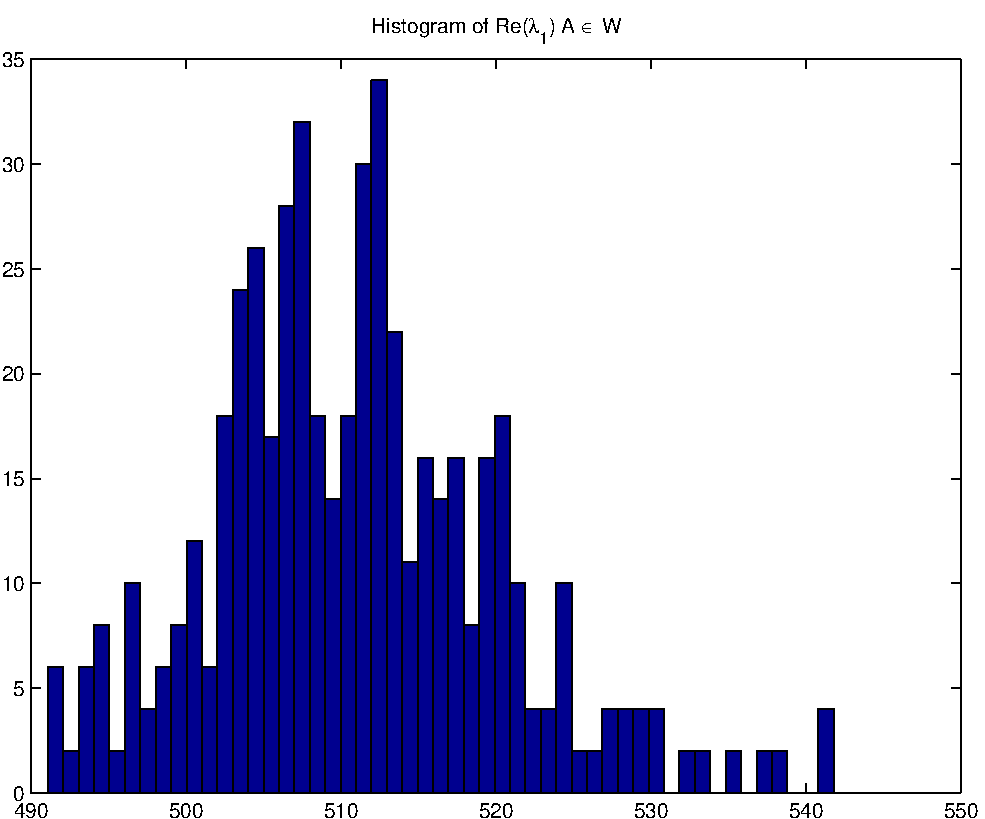
\includegraphics[width=10.0cm,height=10.0cm]{Re_TraceyWidom.pdf}

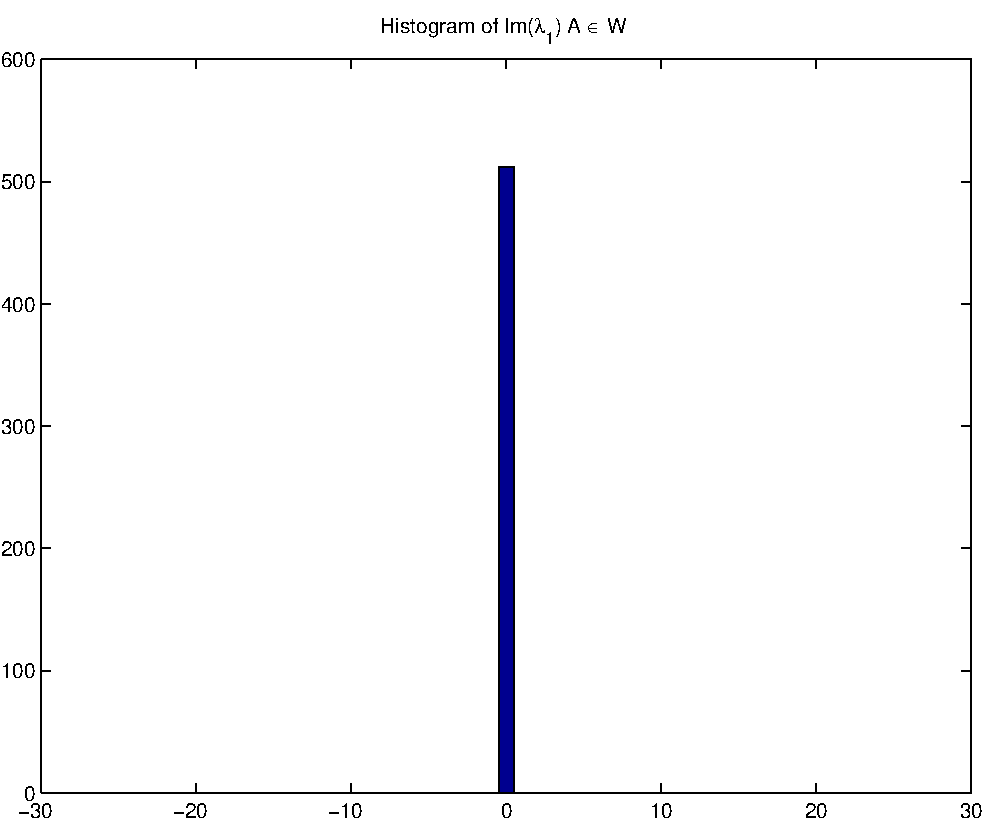
\includegraphics[width=10.0cm,height=10.0cm]{Im_TraceyWidom.pdf}

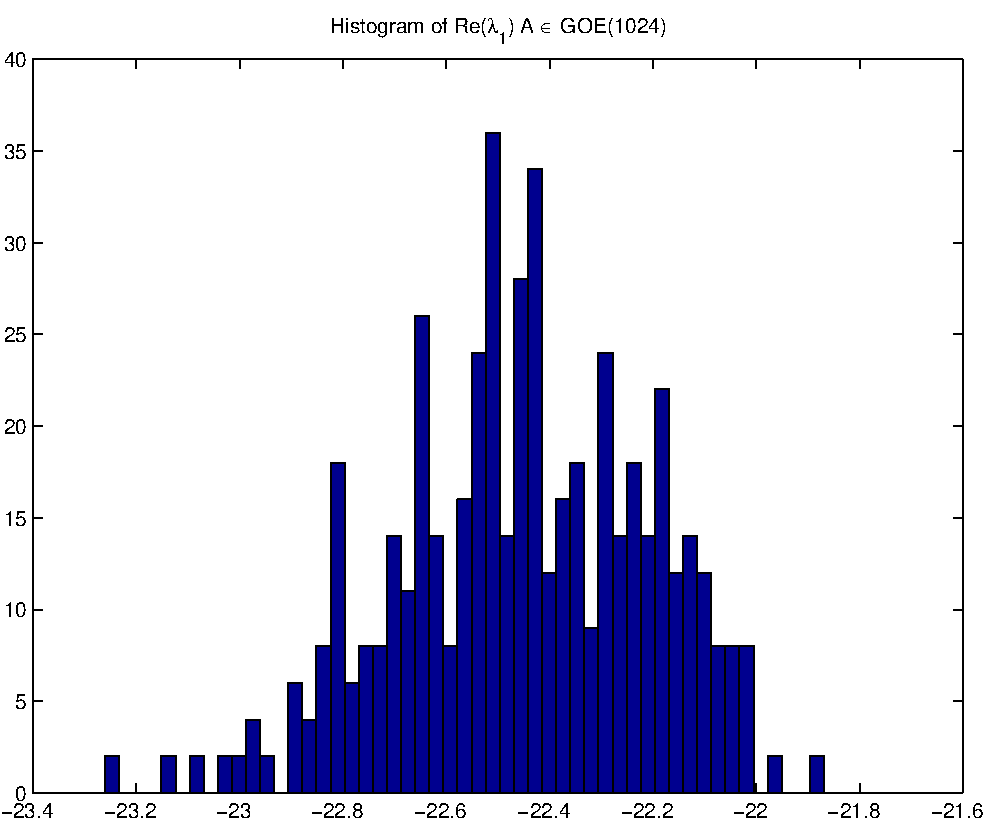
\includegraphics[width=10.0cm,height=10.0cm]{Re_Winger.pdf}

\includegraphics[width=10.0cm,height=10.0cm]{Im_Winger.pdf}

QueryPerformanceCounter  =  +5.272
\subsubsection{Approximate Winger Distribution}
\subsubsection{Verfy Winger Law.}
Let $M_n = [X_{ij} ]$ a symmetric n x n matrix with Random entries such that $X_{i,j} = X_{j,i}$, 		  and $X_{i,j}$ are iid $orall i < j,$ and $Xjj$ are iid $orall j  :  ; E[X^2_{ij} ] = 1, & E[X_{ij}] = 0$ 		  and that all moments exists for each of the entries.  		  The eigenvector of this random matrix; $ lambda_1 leq ... leq lambda_n$ depends continuously on $Mn$.
Dimension $n = +512$

\includegraphics[width=10.0cm,height=10.0cm]{Re_lambda_n.pdf}

\includegraphics[width=10.0cm,height=10.0cm]{Im_lambda_n.pdf}

QueryPerformanceCounter  =  +2.921
\subsubsection{Matrix Exponential }
$SPD Matrix = \left(
\begin{array}{
cccccccc}
+10.539 & -0.499 & -0.010 & +0.368 & +0.465 & -0.492 & -0.126 & +0.437 \\
-0.499 & +7.286 & +0.365 & -0.481 & -0.337 & -0.466 & +0.279 & +0.056 \\
-0.010 & +0.365 & +6.705 & -0.205 & +0.467 & +0.131 & +0.077 & -0.089 \\
+0.368 & -0.481 & -0.205 & +6.496 & -0.402 & -0.209 & +0.043 & -0.041 \\
+0.465 & -0.337 & +0.467 & -0.402 & +4.578 & +0.272 & +0.289 & -0.285 \\
-0.492 & -0.466 & +0.131 & -0.209 & +0.272 & +8.181 & +0.343 & -0.244 \\
-0.126 & +0.279 & +0.077 & +0.043 & +0.289 & +0.343 & +5.938 & -0.212 \\
+0.437 & +0.056 & -0.089 & -0.041 & -0.285 & -0.244 & -0.212 & +9.691 \\
\end{array}
\right)$ \newline 

$SPD Eigs = \left(
\begin{array}{
cccccccc}
(+10.93611,+0.00000) & (+9.60778,+0.00000) & (+4.23666,+0.00000) & (+8.36911,+0.00000) & (+7.56229,+0.00000) & (+5.82791,+0.00000) & (+6.54198,+0.00000) & (+6.33139,+0.00000) \\
\end{array}
\right)$ \newline 

$exp(SPD) = \left(
\begin{array}{
cccccccc}
+47863.969 & -6460.093 & -1078.770 & +4706.958 & +2535.224 & -8475.398 & -2406.368 & +12977.552 \\
-6460.093 & +2780.574 & +516.920 & -1069.918 & -548.083 & -109.707 & +386.466 & -807.216 \\
-1078.770 & +516.920 & +1015.281 & -385.755 & +176.069 & +458.541 & +212.284 & -859.022 \\
+4706.958 & -1069.918 & -385.755 & +1267.210 & +111.181 & -1018.272 & -287.809 & +1036.628 \\
+2535.224 & -548.083 & +176.069 & +111.181 & +413.265 & +135.193 & +45.490 & -502.411 \\
-8475.398 & -109.707 & +458.541 & -1018.272 & +135.193 & +5613.026 & +968.003 & -4270.737 \\
-2406.368 & +386.466 & +212.284 & -287.809 & +45.490 & +968.003 & +632.432 & -1645.725 \\
+12977.552 & -807.216 & -859.022 & +1036.628 & -502.411 & -4270.737 & -1645.725 & +19362.944 \\
\end{array}
\right)$ \newline 

$exp(SPD) eigs = \left(
\begin{array}{
cccccccc}
(+56168.17045,+0.00000) & (+14880.07985,+0.00000) & (+4311.77579,+0.00000) & (+1924.25027,+0.00000) & (+69.17669,+0.00000) & (+339.64809,+0.00000) & (+693.66208,+0.00000) & (+561.93669,+0.00000) \\
\end{array}
\right)$ \newline 

$log(exp(SPD) eigs)  = \left(
\begin{array}{
cccccccc}
(+10.93611,+0.00000) & (+9.60778,+0.00000) & (+8.36911,+0.00000) & (+7.56229,+0.00000) & (+4.23666,+0.00000) & (+5.82791,+0.00000) & (+6.54198,+0.00000) & (+6.33139,+0.00000) \\
\end{array}
\right)$ \newline 

$exp(Id) = \left(
\begin{array}{
cccccccc}
+2.718 & +0.000 & +0.000 & +0.000 & +0.000 & +0.000 & +0.000 & +0.000 \\
+0.000 & +2.718 & +0.000 & +0.000 & +0.000 & +0.000 & +0.000 & +0.000 \\
+0.000 & +0.000 & +2.718 & +0.000 & +0.000 & +0.000 & +0.000 & +0.000 \\
+0.000 & +0.000 & +0.000 & +2.718 & +0.000 & +0.000 & +0.000 & +0.000 \\
+0.000 & +0.000 & +0.000 & +0.000 & +2.718 & +0.000 & +0.000 & +0.000 \\
+0.000 & +0.000 & +0.000 & +0.000 & +0.000 & +2.718 & +0.000 & +0.000 \\
+0.000 & +0.000 & +0.000 & +0.000 & +0.000 & +0.000 & +2.718 & +0.000 \\
+0.000 & +0.000 & +0.000 & +0.000 & +0.000 & +0.000 & +0.000 & +2.718 \\
\end{array}
\right)$ \newline 

$exp(Id) eigs = \left(
\begin{array}{
cccccccc}
(+2.71828,+0.00000) & (+2.71828,+0.00000) & (+2.71828,+0.00000) & (+2.71828,+0.00000) & (+2.71828,+0.00000) & (+2.71828,+0.00000) & (+2.71828,+0.00000) & (+2.71828,+0.00000) \\
\end{array}
\right)$ \newline 

$log(exp(Id) eigs)  = \left(
\begin{array}{
cccccccc}
(+1.00000,+0.00000) & (+1.00000,+0.00000) & (+1.00000,+0.00000) & (+1.00000,+0.00000) & (+1.00000,+0.00000) & (+1.00000,+0.00000) & (+1.00000,+0.00000) & (+1.00000,+0.00000) \\
\end{array}
\right)$ \newline 

For $n  \in  \dblz [16,128)$ we calculate  $|( SPD(n) Eigs - log(exp(SPD(n)) eigs)|_{l^2}$

$|( SPD(n) Eigs - log(exp(SPD(n)) eigs)|_{l^2} = \left(
\begin{array}{
cccccccccccccccccccccccccccccccccccccccccccccccccccccccccccccccccccccccccccccccccccccccccccccccccccccccccccccccc}
(+5.36543,+0.00000) & (+5.36543,+0.00000) & (+5.36543,+0.00000) & (+5.36543,+0.00000) & (+5.36543,+0.00000) & (+5.36543,+0.00000) & (+5.36543,+0.00000) & (+5.36543,+0.00000) & (+5.36543,+0.00000) & (+5.36543,+0.00000) & (+5.36543,+0.00000) & (+5.36543,+0.00000) & (+5.36543,+0.00000) & (+5.36543,+0.00000) & (+5.36543,+0.00000) & (+5.36543,+0.00000) & (+5.36543,+0.00000) & (+5.36543,+0.00000) & (+5.36543,+0.00000) & (+5.36543,+0.00000) & (+5.36543,+0.00000) & (+5.36543,+0.00000) & (+5.36543,+0.00000) & (+5.36543,+0.00000) & (+5.36543,+0.00000) & (+5.36543,+0.00000) & (+5.36543,+0.00000) & (+5.36543,+0.00000) & (+5.36543,+0.00000) & (+5.36543,+0.00000) & (+5.36543,+0.00000) & (+5.36543,+0.00000) & (+5.36543,+0.00000) & (+5.36543,+0.00000) & (+5.36543,+0.00000) & (+5.36543,+0.00000) & (+5.36543,+0.00000) & (+5.36543,+0.00000) & (+5.36543,+0.00000) & (+5.36543,+0.00000) & (+5.36543,+0.00000) & (+5.36543,+0.00000) & (+5.36543,+0.00000) & (+5.36543,+0.00000) & (+5.36543,+0.00000) & (+5.36543,+0.00000) & (+5.36543,+0.00000) & (+5.36543,+0.00000) & (-2.44429,+0.00000) & (-2.23416,+0.00000) & (-2.12272,+0.00000) & (-1.68408,+0.00000) & (-1.46701,+0.00000) & (-1.42424,+0.00000) & (-1.19344,+0.00000) & (-1.00106,+0.00000) & (-0.79899,+0.00000) & (-1.32863,+0.00000) & (-0.03334,+0.00000) & (-0.18953,+0.00000) & (-0.70439,+0.00000) & (-0.53235,+0.00000) & (-0.34237,+0.00000) & (-2.07773,+0.00000) & (-0.59962,+0.00000) & (+11.22991,+0.00000) & (+10.41441,+0.00000) & (+10.46783,+0.00000) & (+9.90149,+0.00000) & (+9.80254,+0.00000) & (+9.43560,+0.00000) & (+9.32668,+0.00000) & (+8.69531,+0.00000) & (+8.60839,+0.00000) & (+8.50649,+0.00000) & (+8.10449,+0.00000) & (+8.00930,+0.00000) & (+7.80818,+0.00000) & (+7.62980,+0.00000) & (+7.49638,+0.00000) & (+7.27792,+0.00000) & (+7.03568,+0.00000) & (+6.93971,+0.00000) & (+6.68496,+0.00000) & (+6.65899,+0.00000) & (+6.18603,+0.00000) & (+6.36871,+0.00000) & (+6.35404,+0.00000) & (+5.89747,+0.00000) & (+5.79944,+0.00000) & (+5.64551,+0.00000) & (+5.48740,+0.00000) & (+5.39983,+0.00000) & (+5.21111,+0.00000) & (+5.10213,+0.00000) & (+5.05172,+0.00000) & (+4.79593,+0.00000) & (+4.74556,+0.00000) & (+4.57093,+0.00000) & (+4.35876,+0.00000) & (+3.88183,+0.00000) & (+4.00029,+0.00000) & (+3.64260,+0.00000) & (+3.45729,+0.00000) & (+3.28400,+0.00000) & (+3.19484,+0.00000) & (+3.07091,+0.00000) & (+2.94105,+0.00000) & (+2.86247,+0.00000) & (+2.58917,+0.00000) & (+2.40251,+0.00000) & (+2.34452,+0.00000) \\
\end{array}
\right)$ \newline 

QueryPerformanceCounter  =  +0.00985
The sample size generated for this run is 100000.

\newpage
uniform \begin{tabular}{|c|c|c|c|}  mean & variance & skewness & kurtosis \\  \hline
$\mu_1 = +0.50030$ & $\mu_2 = +0.08353$ & $\mu_3 = +0.00339$ & $\mu_4 =+1.80113$ \\
\end{tabular}

\includegraphics[width=5cm,height=5cm]{uniform.pdf}

cauchy \begin{tabular}{|c|c|c|c|}  mean & variance & skewness & kurtosis \\  \hline
$\mu_1 = +0.44288$ & $\mu_2 = +0.05341$ & $\mu_3 = +0.63935$ & $\mu_4 =+3.28094$ \\
\end{tabular}

\includegraphics[width=5cm,height=5cm]{cauchy.pdf}

exponential \begin{tabular}{|c|c|c|c|}  mean & variance & skewness & kurtosis \\  \hline
$\mu_1 = +1.99647$ & $\mu_2 = +3.99339$ & $\mu_3 = +2.03097$ & $\mu_4 =+9.30842$ \\
\end{tabular}

\includegraphics[width=5cm,height=5cm]{exponential.pdf}

\newpage
gamma \begin{tabular}{|c|c|c|c|}  mean & variance & skewness & kurtosis \\  \hline
$\mu_1 = +1.90890$ & $\mu_2 = +1.93504$ & $\mu_3 = +1.46913$ & $\mu_4 =+6.24391$ \\
\end{tabular}

\includegraphics[width=5cm,height=5cm]{gamma.pdf}

GIG \begin{tabular}{|c|c|c|c|}  mean & variance & skewness & kurtosis \\  \hline
$\mu_1 = +0.80307$ & $\mu_2 = +11.06705$ & $\mu_3 = +15.24671$ & $\mu_4 =+312.50419$ \\
\end{tabular}

\includegraphics[width=5cm,height=5cm]{GIG.pdf}

normal-box-muller \begin{tabular}{|c|c|c|c|}  mean & variance & skewness & kurtosis \\  \hline
$\mu_1 = +0.00070$ & $\mu_2 = +0.99290$ & $\mu_3 = +0.00421$ & $\mu_4 =+2.95755$ \\
\end{tabular}

\includegraphics[width=5cm,height=5cm]{normal-box-muller.pdf}

\newpage
normal-inverse-approximation \begin{tabular}{|c|c|c|c|}  mean & variance & skewness & kurtosis \\  \hline
$\mu_1 = +0.00230$ & $\mu_2 = +1.00486$ & $\mu_3 = +0.01163$ & $\mu_4 =+2.99254$ \\
\end{tabular}

\includegraphics[width=5cm,height=5cm]{normal-inverse-approximation.pdf}

pareto \begin{tabular}{|c|c|c|c|}  mean & variance & skewness & kurtosis \\  \hline
$\mu_1 = +3184578.26493$ & $\mu_2 = +888468246174112900.00000$ & $\mu_3 = +315.36997$ & $\mu_4 =+99629.09819$ \\
\end{tabular}

\includegraphics[width=5cm,height=5cm]{pareto.pdf}

poisson \begin{tabular}{|c|c|c|c|}  mean & variance & skewness & kurtosis \\  \hline
$\mu_1 = +1.10547$ & $\mu_2 = +0.13097$ & $\mu_3 = +3.96445$ & $\mu_4 =+21.71364$ \\
\end{tabular}

\includegraphics[width=5cm,height=5cm]{poisson.pdf}

\newpage
beta \begin{tabular}{|c|c|c|c|}  mean & variance & skewness & kurtosis \\  \hline
$\mu_1 = +0.33346$ & $\mu_2 = +0.12755$ & $\mu_3 = +0.68178$ & $\mu_4 =+1.90650$ \\
\end{tabular}

\includegraphics[width=5cm,height=5cm]{beta.pdf}

QueryPerformanceCounter  =  +11.03008
\subsubsection{Multiclass Support Vector Machine }
\begin{itemize}
\item Number or training points = 1024
\item Feature dimension = 3
\item Number or classes = 3
\end{itemize}
{The mean vectors of the 3 classes}

$\mu_1 = \left(
\begin{array}{
ccc}
+1.90000 & +0.10000 & +0.10000 \\
\end{array}
\right)$ \newline 

$\mu_2 = \left(
\begin{array}{
ccc}
+0.10000 & +1.90000 & +0.10000 \\
\end{array}
\right)$ \newline 

$\mu_3 = \left(
\begin{array}{
ccc}
+0.00000 & +0.00000 & +1.90000 \\
\end{array}
\right)$ \newline 

A random SPD covairance matrix is generated for each of the classes.\newline

$\rho_1 = \left(
\begin{array}{
ccc}
+3.141 & -0.122 & +0.142 \\
-0.122 & +4.448 & -0.432 \\
+0.142 & -0.432 & +2.050 \\
\end{array}
\right)$ \newline 

$\rho_2 = \left(
\begin{array}{
ccc}
+1.735 & +0.369 & +0.024 \\
+0.369 & +4.351 & -0.232 \\
+0.024 & -0.232 & +2.437 \\
\end{array}
\right)$ \newline 

$\rho_3 = \left(
\begin{array}{
ccc}
+4.334 & -0.269 & -0.316 \\
-0.269 & +3.777 & +0.215 \\
-0.316 & +0.215 & +1.581 \\
\end{array}
\right)$ \newline 

Verify $L_1$ condition number of covariance. The diagonal entries of the matrix have the form $(0.5 + U(0,1) )*dim(Dom(Cov))$
The lower-diagonal entries take the form $U(0,1) - 0.5$. 
The $L_1$ condition numbers are :
\begin{itemize}
\item +2.840
\item +3.211
\item +3.564
\end{itemize}
\includegraphics[width=10.0cm,height=10.0cm]{rv1_corr.pdf}

\includegraphics[width=10.0cm,height=10.0cm]{rv2_corr.pdf}

\includegraphics[width=10.0cm,height=10.0cm]{rv3_corr.pdf}

\includegraphics[width=10.0cm,height=10.0cm]{trainingPoints.pdf}

These are the SVM parameters - the RBF kernel is used\begin{itemize}
\item allOutlierFraction=0.05
\item mixingCoeff=0.3
\item smoThresh=1.0/10000.0
\item sigma=1
\end{itemize}
\includegraphics[width=10.0cm,height=10.0cm]{testPoints.pdf}

The marginal sample moments (mean var skew kurtosis) for training points.\newline
\begin{tabular}{ c |  c  c  c  c}
Feature & $\mu_1$ & $\mu_2$ & $\mu_3$ & $\mu_4$ \\
0 & +0.669 & +1.374 & +0.220& +2.455 \\
\hline
1 & +0.710 & +1.485 & +0.327& +2.545 \\
\hline
2 & +0.698 & +1.127 & +0.263& +2.159 \\
\hline
\end{tabular}
\newline
The marginal sample moments (mean var skew kurtosis) for test points.\newline
\begin{tabular}{ c | c  c  c  c}
Feature & $\mu_1$ & $\mu_2$ & $\mu_3$ & $\mu_4$ \\
0 & +0.677 & +1.286 & +0.340& +2.595\\
\hline
1 & +0.669 & +1.480 & +0.341& +2.550\\
\hline
2 & +0.720 & +1.070 & +0.256& +2.102\\
\hline
\end{tabular}\newline
\includegraphics[width=10.0cm,height=10.0cm]{classDiffs.pdf}

The error rate for this run is +0.173\newline
QueryPerformanceCounter  =  +6.380
\subsubsection{Semidefinite Programming SDPA}
QueryPerformanceCounter  =  +0.005
\end{document}
